% Options for packages loaded elsewhere
\PassOptionsToPackage{unicode}{hyperref}
\PassOptionsToPackage{hyphens}{url}
%
\documentclass[
]{article}
\usepackage{amsmath,amssymb}
\usepackage{iftex}
\ifPDFTeX
  \usepackage[T1]{fontenc}
  \usepackage[utf8]{inputenc}
  \usepackage{textcomp} % provide euro and other symbols
\else % if luatex or xetex
  \usepackage{unicode-math} % this also loads fontspec
  \defaultfontfeatures{Scale=MatchLowercase}
  \defaultfontfeatures[\rmfamily]{Ligatures=TeX,Scale=1}
\fi
\usepackage{lmodern}
\ifPDFTeX\else
  % xetex/luatex font selection
\fi
% Use upquote if available, for straight quotes in verbatim environments
\IfFileExists{upquote.sty}{\usepackage{upquote}}{}
\IfFileExists{microtype.sty}{% use microtype if available
  \usepackage[]{microtype}
  \UseMicrotypeSet[protrusion]{basicmath} % disable protrusion for tt fonts
}{}
\makeatletter
\@ifundefined{KOMAClassName}{% if non-KOMA class
  \IfFileExists{parskip.sty}{%
    \usepackage{parskip}
  }{% else
    \setlength{\parindent}{0pt}
    \setlength{\parskip}{6pt plus 2pt minus 1pt}}
}{% if KOMA class
  \KOMAoptions{parskip=half}}
\makeatother
\usepackage{xcolor}
\usepackage[margin=1in]{geometry}
\usepackage{color}
\usepackage{fancyvrb}
\newcommand{\VerbBar}{|}
\newcommand{\VERB}{\Verb[commandchars=\\\{\}]}
\DefineVerbatimEnvironment{Highlighting}{Verbatim}{commandchars=\\\{\}}
% Add ',fontsize=\small' for more characters per line
\usepackage{framed}
\definecolor{shadecolor}{RGB}{248,248,248}
\newenvironment{Shaded}{\begin{snugshade}}{\end{snugshade}}
\newcommand{\AlertTok}[1]{\textcolor[rgb]{0.94,0.16,0.16}{#1}}
\newcommand{\AnnotationTok}[1]{\textcolor[rgb]{0.56,0.35,0.01}{\textbf{\textit{#1}}}}
\newcommand{\AttributeTok}[1]{\textcolor[rgb]{0.13,0.29,0.53}{#1}}
\newcommand{\BaseNTok}[1]{\textcolor[rgb]{0.00,0.00,0.81}{#1}}
\newcommand{\BuiltInTok}[1]{#1}
\newcommand{\CharTok}[1]{\textcolor[rgb]{0.31,0.60,0.02}{#1}}
\newcommand{\CommentTok}[1]{\textcolor[rgb]{0.56,0.35,0.01}{\textit{#1}}}
\newcommand{\CommentVarTok}[1]{\textcolor[rgb]{0.56,0.35,0.01}{\textbf{\textit{#1}}}}
\newcommand{\ConstantTok}[1]{\textcolor[rgb]{0.56,0.35,0.01}{#1}}
\newcommand{\ControlFlowTok}[1]{\textcolor[rgb]{0.13,0.29,0.53}{\textbf{#1}}}
\newcommand{\DataTypeTok}[1]{\textcolor[rgb]{0.13,0.29,0.53}{#1}}
\newcommand{\DecValTok}[1]{\textcolor[rgb]{0.00,0.00,0.81}{#1}}
\newcommand{\DocumentationTok}[1]{\textcolor[rgb]{0.56,0.35,0.01}{\textbf{\textit{#1}}}}
\newcommand{\ErrorTok}[1]{\textcolor[rgb]{0.64,0.00,0.00}{\textbf{#1}}}
\newcommand{\ExtensionTok}[1]{#1}
\newcommand{\FloatTok}[1]{\textcolor[rgb]{0.00,0.00,0.81}{#1}}
\newcommand{\FunctionTok}[1]{\textcolor[rgb]{0.13,0.29,0.53}{\textbf{#1}}}
\newcommand{\ImportTok}[1]{#1}
\newcommand{\InformationTok}[1]{\textcolor[rgb]{0.56,0.35,0.01}{\textbf{\textit{#1}}}}
\newcommand{\KeywordTok}[1]{\textcolor[rgb]{0.13,0.29,0.53}{\textbf{#1}}}
\newcommand{\NormalTok}[1]{#1}
\newcommand{\OperatorTok}[1]{\textcolor[rgb]{0.81,0.36,0.00}{\textbf{#1}}}
\newcommand{\OtherTok}[1]{\textcolor[rgb]{0.56,0.35,0.01}{#1}}
\newcommand{\PreprocessorTok}[1]{\textcolor[rgb]{0.56,0.35,0.01}{\textit{#1}}}
\newcommand{\RegionMarkerTok}[1]{#1}
\newcommand{\SpecialCharTok}[1]{\textcolor[rgb]{0.81,0.36,0.00}{\textbf{#1}}}
\newcommand{\SpecialStringTok}[1]{\textcolor[rgb]{0.31,0.60,0.02}{#1}}
\newcommand{\StringTok}[1]{\textcolor[rgb]{0.31,0.60,0.02}{#1}}
\newcommand{\VariableTok}[1]{\textcolor[rgb]{0.00,0.00,0.00}{#1}}
\newcommand{\VerbatimStringTok}[1]{\textcolor[rgb]{0.31,0.60,0.02}{#1}}
\newcommand{\WarningTok}[1]{\textcolor[rgb]{0.56,0.35,0.01}{\textbf{\textit{#1}}}}
\usepackage{longtable,booktabs,array}
\usepackage{calc} % for calculating minipage widths
% Correct order of tables after \paragraph or \subparagraph
\usepackage{etoolbox}
\makeatletter
\patchcmd\longtable{\par}{\if@noskipsec\mbox{}\fi\par}{}{}
\makeatother
% Allow footnotes in longtable head/foot
\IfFileExists{footnotehyper.sty}{\usepackage{footnotehyper}}{\usepackage{footnote}}
\makesavenoteenv{longtable}
\usepackage{graphicx}
\makeatletter
\newsavebox\pandoc@box
\newcommand*\pandocbounded[1]{% scales image to fit in text height/width
  \sbox\pandoc@box{#1}%
  \Gscale@div\@tempa{\textheight}{\dimexpr\ht\pandoc@box+\dp\pandoc@box\relax}%
  \Gscale@div\@tempb{\linewidth}{\wd\pandoc@box}%
  \ifdim\@tempb\p@<\@tempa\p@\let\@tempa\@tempb\fi% select the smaller of both
  \ifdim\@tempa\p@<\p@\scalebox{\@tempa}{\usebox\pandoc@box}%
  \else\usebox{\pandoc@box}%
  \fi%
}
% Set default figure placement to htbp
\def\fps@figure{htbp}
\makeatother
\setlength{\emergencystretch}{3em} % prevent overfull lines
\providecommand{\tightlist}{%
  \setlength{\itemsep}{0pt}\setlength{\parskip}{0pt}}
\setcounter{secnumdepth}{5}
\usepackage{color}
\usepackage{tcolorbox}

\definecolor{berkeleyblue}{HTML}{003262}
\definecolor{berkeleygold}{HTML}{FDB515}
\definecolor{bayfog}{HTML}{DDD5C7}
\definecolor{laplane}{HTML}{00A598}
\definecolor{ion}{HTML}{CFDD45}
\definecolor{sathergate}{HTML}{B9D3B6}
\definecolor{stonepine}{HTML}{584F29}

\newtcolorbox{breakout}{
  colback=berkeleyblue,
  colframe=berkeleygold,
  coltext=white,
  boxsep=5pt,
  arc=4pt
}

\newtcolorbox{discussion-question}{
  colback=bayfog,
  colframe=laplane,
  coltext=laplane,
  boxsep=5pt,
  arc=4pt
}

% \newtcolorbox{definition}{
%   colback=ion,
%   colframe=stonepine,
%   coltext=stonepine,
%   boxsep=5pt,
%   arc=4pt
% }

% \newtcolorbox{theorem}{
%   colback=sathergate,
%   colframe=stonepine,
%   coltext=stonepine,
%   boxsep=5pt,
%   arc=4pt
% }
\usepackage{bookmark}
\IfFileExists{xurl.sty}{\usepackage{xurl}}{} % add URL line breaks if available
\urlstyle{same}
\hypersetup{
  pdftitle={Experiments and Causality},
  pdfauthor={The 241 Instructional Team},
  hidelinks,
  pdfcreator={LaTeX via pandoc}}

\title{Experiments and Causality}
\author{The 241 Instructional Team\footnote{David Reiley, D. Alex Hughes, David Broockman, Micah Gell-Redman, Scott Guenther, David Wheeler, Josue Martinez, Maya Duru}}
\date{2024-11-12}

\usepackage{amsthm}
\newtheorem{theorem}{Theorem}[section]
\newtheorem{lemma}{Lemma}[section]
\newtheorem{corollary}{Corollary}[section]
\newtheorem{proposition}{Proposition}[section]
\newtheorem{conjecture}{Conjecture}[section]
\theoremstyle{definition}
\newtheorem{definition}{Definition}[section]
\theoremstyle{definition}
\newtheorem{example}{Example}[section]
\theoremstyle{definition}
\newtheorem{exercise}{Exercise}[section]
\theoremstyle{definition}
\newtheorem{hypothesis}{Hypothesis}[section]
\theoremstyle{remark}
\newtheorem*{remark}{Remark}
\newtheorem*{solution}{Solution}
\begin{document}
\maketitle

{
\setcounter{tocdepth}{2}
\tableofcontents
}
\section*{Live Session Introduction}\label{live-session-introduction}
\addcontentsline{toc}{section}{Live Session Introduction}

This is the live session work space for the course. Our goal with this repository, is that we're able to communicate \emph{ahead of time} our aims for each week, and that you can prepare accordingly.

\subsection*{Bloom's Taxonomy}\label{blooms-taxonomy}
\addcontentsline{toc}{subsection}{Bloom's Taxonomy}

An effective rubric for student understanding is attributed to Bloom (1956). Referred to as \emph{Bloom's Taxonomy}, this proposes that there is a hierarchy of student understanding; that a student may have one \emph{level} of reasoning skill with a concept, but not another. The taxonomy proposes to be ordered: some levels of reasoning build upon other levels of reasoning.

In the learning objective that we present in for each live session, we will also identify the level of reasoning that we hope students will achieve at the conclusion of the live session.

\begin{enumerate}
\def\labelenumi{\arabic{enumi}.}
\tightlist
\item
  \textbf{Remember} A student can remember that the concept exists. This might require the student to define, duplicate, or memorize a set of concepts or facts.
\item
  \textbf{Understand} A student can understand the concept, and can produce a working technical and non-technical statement of the concept. The student can explain why the concept \emph{is}, or why the concept works in the way that it does.
\item
  \textbf{Apply} A student can use the concept as it is intended to be used against a novel problem.
\item
  \textbf{Analyze} A student can assess whether the concept has worked as it should have. This requires both an understanding of the intended goal, an application against a novel problem, and then the ability to introspect or reflect on whether the result is as it should be.
\item
  \textbf{Evaluate} A student can analyze multiple approaches, and from this analysis evaluate whether one or another approach has better succeeded at achieving its goals.
\item
  \textbf{Create} A student can create a new or novel method from axioms or experience, and can evaluate the performance of this new method against existing approaches or methods.
\end{enumerate}

\section{Importance of Experimentation}\label{importance-of-experimentation}

\begin{figure}
\centering
\pandocbounded{\includegraphics[keepaspectratio]{./images/point_reyes.jpg}}
\caption{Point Reyes National Seashore}
\end{figure}

\subsection{Core Questions}\label{core-questions}

This course is about designing experiments that we run in the \emph{real-world}.

\begin{itemize}
\tightlist
\item
  What is the value of making a causal statement?
\item
  Why do we conduct experiments?
\item
  This is a data science program. With enough data and a savvy enough model, can't we just generate a causal statement that will be right? Can't I generate a statement that converges in probability to the \emph{correct} value?
\end{itemize}

\subsection{Learning Objectives}\label{learning-objectives}

At the end of this live session, students will be able to

\begin{enumerate}
\def\labelenumi{\arabic{enumi}.}
\tightlist
\item
  \emph{Remember} (or find) the goals of the course, the assessment structure, and the learning model.
\item
  \emph{Define}, in non-technical language, what it means for an action to cause an outcome.
\item
  \emph{Understand} the difference between a causal statement, and an association statement.
\item
  \emph{Apply} the framework of causal thinking against a series of studies to determine whether the study has achieved the goal that it intends.
\end{enumerate}

\subsection{Class Introductions}\label{class-introductions}

\subsection{Student Introductions {[}Breakout One{]}}\label{student-introductions-breakout-one}

In a breakout room of between three and four students introduce yourself!

\begin{breakout}
\textbf{Breakout One.} A \emph{name story} is the unique, and individual story that describes how you came to have the name that you do. While there may be many people are called the same thing, each of their name stories is unique.

Please share: \emph{What is your name story?}

\end{breakout}

\subsection{Student Introductions {[}Breakout Two{]}}\label{student-introductions-breakout-two}

In the same breakout room:

\begin{breakout}
\textbf{Breakout Two.}
Like our names, the reasons that we joined this program, our goals and our histories are different.

Please share: \emph{What is your data science story? How did you wind up here, in this room today?}

\end{breakout}

\subsection{Course Plan}\label{course-plan}

The course is built out into three distinct phases

\begin{itemize}
\tightlist
\item
  \textbf{Part 1} Develops causal theory, potential outcomes, and a permutation-based uncertainty measurement
\item
  \textbf{Part 2} Further develops the idea of a treatment effect, and teaches how the careful design of experiments can improve the efficiency, and easy of analysis
\item
  \textbf{Part 3} Presents practical considerations when conducting an experiment, including problems that may arise, and how to design an experiment in anticipation of those problems.
\end{itemize}

\subsection{Course Logistics}\label{course-logistics}

\begin{itemize}
\tightlist
\item
  bCourses

  \begin{itemize}
  \tightlist
  \item
    Learning Modules attached to weeks
  \item
    Modules contain async lectures, coding exercises, and quizzes
  \end{itemize}
\item
  GitHub

  \begin{itemize}
  \tightlist
  \item
    All the course materials are available in a GitHub repository
  \item
    We have protected the \texttt{main} branch, so you can't do anything destructive
  \item
    Use that as empowerment! This is your class, propose changes that you would like to see!
  \end{itemize}
\item
  Github Classroom

  \begin{itemize}
  \tightlist
  \item
    Assignments will all be applied programming assignments against simulated and real data
  \item
    All assignment code will be distributed through GitHub Classroom
  \end{itemize}
\item
  Gradescope

  \begin{itemize}
  \tightlist
  \item
    All assignments will be submitted to Gradescope where we'll read your solutions and provide scores and feedback
  \end{itemize}
\end{itemize}

\subsubsection{Learning model for the class}\label{learning-model-for-the-class}

The course assignments are designed to put what we have learned in reading, async, and live session into practice in code. In our ideal version of your studying, we would have you working hard together with your classmates in a study group on the assignments, coming to office hours to talk candidly about what is and isn't working, and then \emph{every single student} arriving at a full solution.

\subsubsection{Feedback model for the class}\label{feedback-model-for-the-class}

We want to get you feedback \emph{very} quickly after you turn your assignments.

\begin{enumerate}
\def\labelenumi{\arabic{enumi}.}
\tightlist
\item
  We will release a solution set the day that you turn your assignment in
\item
  We will hold a problem set debrief office hour the Friday (i.e.~next day) after the problem set it submitted
\item
  We will have light-feedback on your assignments within 7 days of when you submitted them.
\item
  You should bring your assignment to office hours after you have turned it in so that we can talk about any differences between your approach, and the instructors approach.
\end{enumerate}

\subsubsection{Office hour model for the class}\label{office-hour-model-for-the-class}

\begin{itemize}
\tightlist
\item
  We will hold office hours Sunday through Thursday at 5:30.
\item
  We will hold more than 10 hours of office hours every week; they will all be recorded, and any student is welcome in any office hour
\end{itemize}

\subsection{Article Discussion}\label{article-discussion}

\subsubsection{Predict or Cause}\label{predict-or-cause}

\begin{itemize}
\tightlist
\item
  What are a few examples that Athey raises of causal questions masquerading as prediction questions?

  \begin{enumerate}
  \def\labelenumi{\arabic{enumi}.}
  \tightlist
  \item
  \item
  \item
  \end{enumerate}
\item
  Which of these examples is the most surprising to you?
\item
  Is there something that is common to each of these examples? Is this a general phenomenon, or is Athey very clever in picking examples? Said differently, is Athey making a clever argument or is a lot of what we do as data scientists actually causal work in disguise?
\end{itemize}

\subsubsection{Do the suburbs make you fat?}\label{do-the-suburbs-make-you-fat}

\begin{enumerate}
\def\labelenumi{\arabic{enumi}.}
\tightlist
\item
  What is the causal claim being made in this article?
\item
  If you had to draw out this causal claim, using arrows, what would it look like?
\item
  Do you acknowledge the association that the authors present? Is there \emph{actually} a difference between the BMI of people who live in cities and the suburbs?
\item
  If you acknowledge the association, does that compel you to believe the causal claim? Why or why not?
\item
  Name, and draw, five alternative \emph{confounding} variables that might make you skeptical that the claimed relationship exists.
\item
  (Optional) Name, and draw two \emph{mechanisms} that might exist between suburbs and BMI. Why does the existence (or not) of these mechanisms \emph{not} pose a fundamental problem to the causal claim that the authors make?
\item
  At the conclusion of reading this paper, do you believe that there is a causal relationship between location and BMI? If so, what compels you to to believe this; if not, why are you not compelled to believe this?
\end{enumerate}

\subsubsection{Nike Shoes}\label{nike-shoes}

\begin{enumerate}
\def\labelenumi{\arabic{enumi}.}
\tightlist
\item
  What is the causal claim being made in this article?
\item
  If you had to draw out this causal claim, using arrows, what would it look like?
\item
  Do you acknowledge the association that the authors present? Is there actually a difference in the finish time between people who are running with the Nike shoes vs.~other shoes?
\item
  If you acknowledge the association, does that compel you to believe the causal claim? Why or why not?
\item
  What are some of the confounding relationships that the authors identify? (Can you name four?) How do they adjust their analyses once they acknowledge the confounding problem?
\item
  At the conclusion of reading this paper, do you believe that there is a causal relationship between shoes and finish time? If so, what compels you to to believe this; if not, why are you not compelled to believe this?
\end{enumerate}

\subsubsection{What is Science: Feynman's View}\label{what-is-science-feynmans-view}

In \emph{Cargo Cult Science}, Richard Feynman poses a view of science that is about a seeking of the truth.

\begin{enumerate}
\def\labelenumi{\arabic{enumi}.}
\tightlist
\item
  What is Feynman's view of science? What does he think makes something \emph{scientific}?
\item
  What are ways that individuals fool themselves when they are working as scientists? What are ways that individuals fool themselves when they are working as data scientists?
\item
  How can we as (data) scientists, train ourselves not to be fooled?\footnote{This is a footnote, rendered into an html document.}
\end{enumerate}

\section{Apples to Apples}\label{apples-to-apples}

\begin{figure}
\centering
\pandocbounded{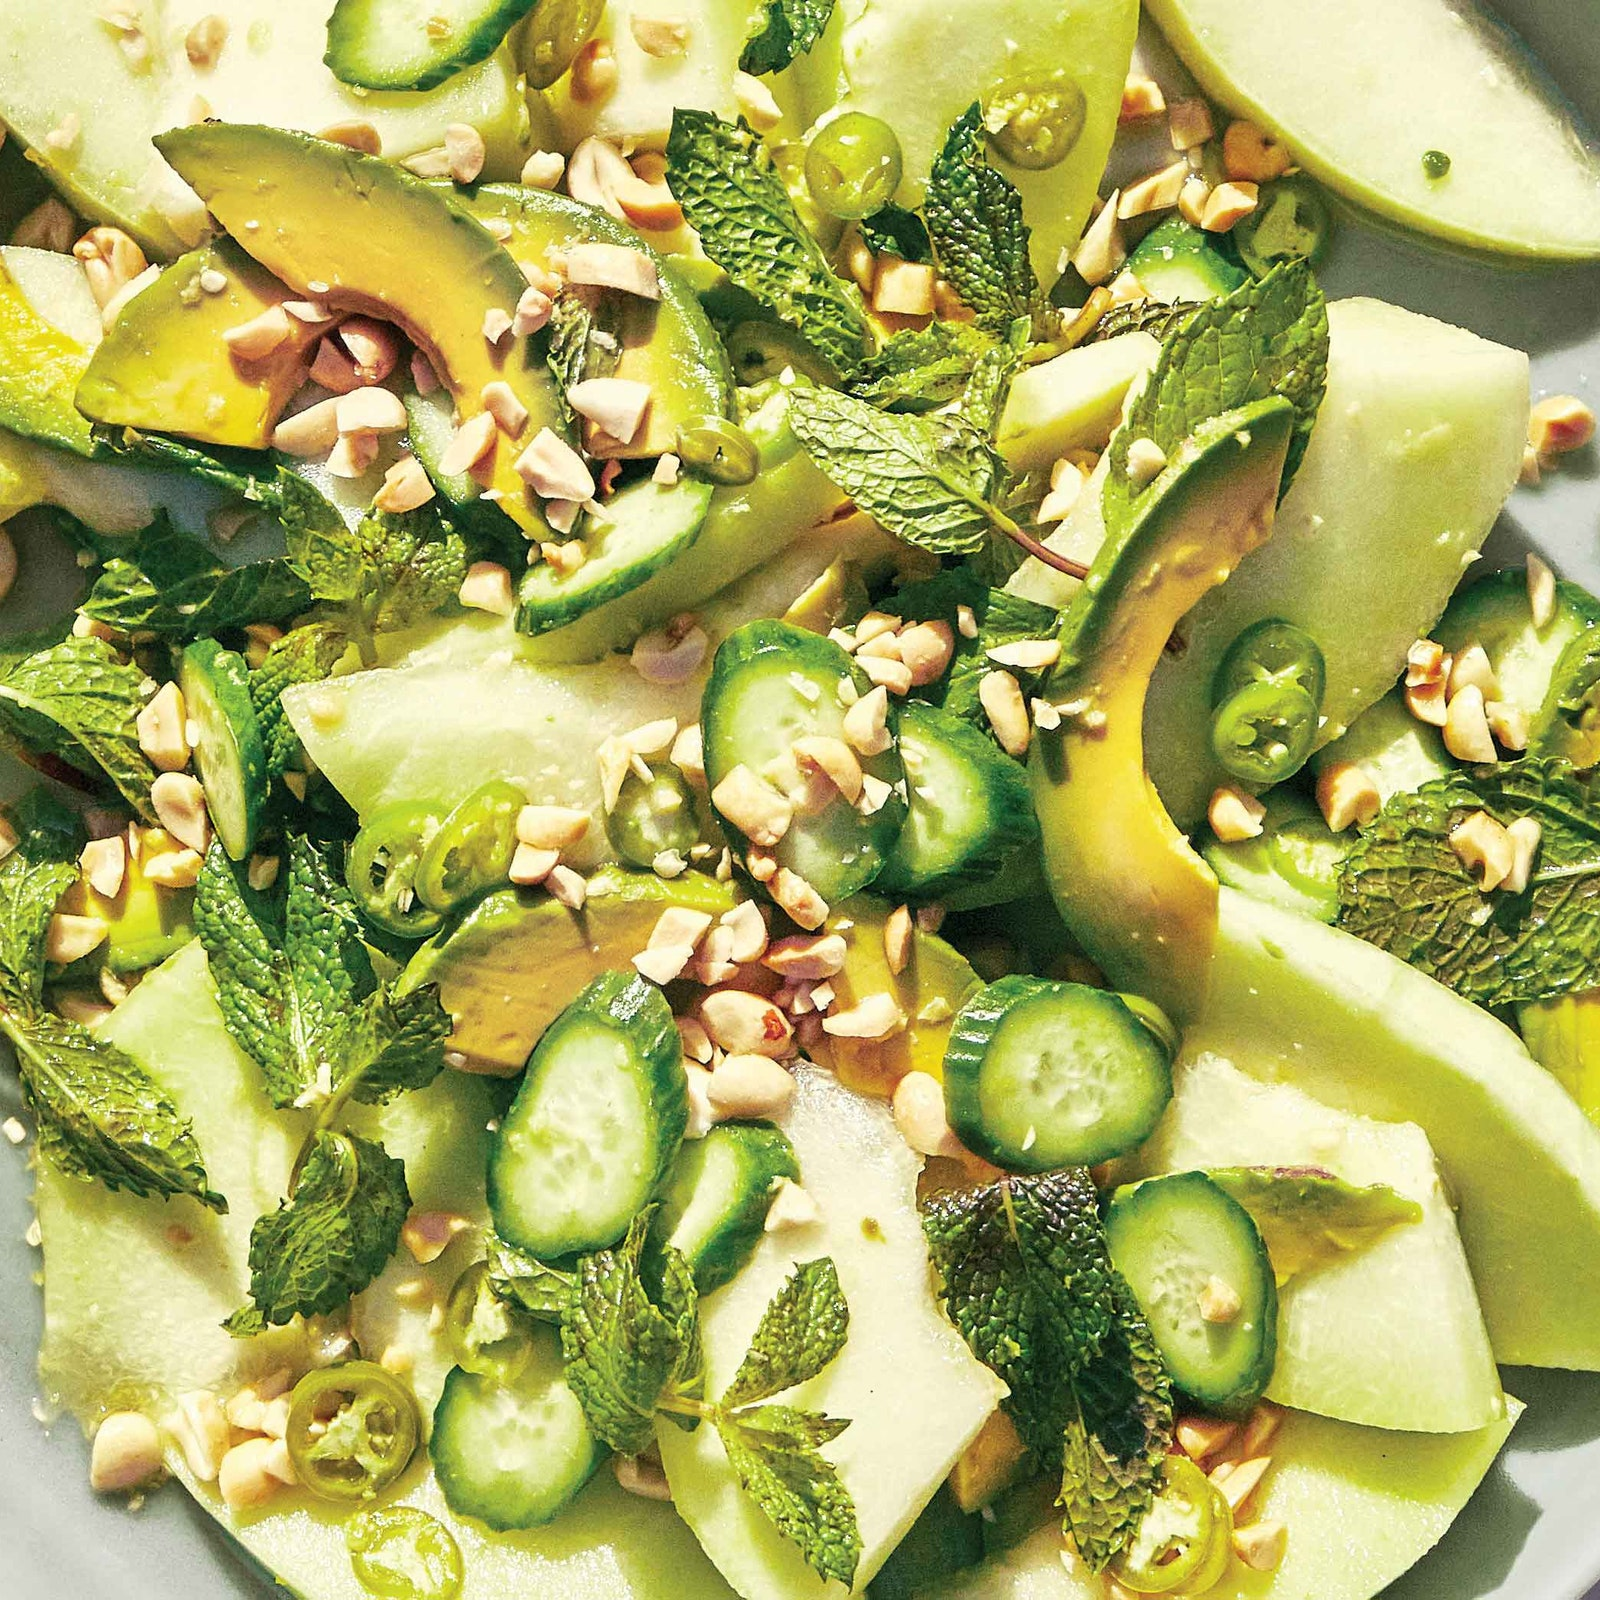
\includegraphics[keepaspectratio]{./images/honeydew-salad-with-ginger-dressing-and-peanuts.jpeg}}
\caption{fruit salad}
\end{figure}

\subsection{Learning Objectives}\label{learning-objectives-1}

At the conclusion of this week's live session, student will be able to:

\begin{enumerate}
\def\labelenumi{\arabic{enumi}.}
\tightlist
\item
  \emph{Describe}, using the technical language of potential outcomes, what it means for an input to \emph{cause} an output.
\item
  \emph{Describe} the fundamental problem of causal inference.
\item
  \emph{Apply} iid sampling as a method of producing an unbiased, consistent estimator of a population.
\item
  \emph{Prove} that the average treatment effect estimator produces an unbiased, consistent estimator for the average treatment effect.
\end{enumerate}

\subsection{Revisiting Ideas of Science}\label{revisiting-ideas-of-science}

Questions about epistemology are a \emph{classic} questions. These questions are particularly relevant here at the School of Information. You're working toward being a data scientist that has a full view of not only how to build the technology, but also for how that technology will behave, alter, and affect the people who use it.

The idea of epistemology -- the idea that some things are known truths, while others are merely opinions -- is perhaps one of the earliest philosophical (i.e.~academic questions).

\begin{quote}
\emph{What does it mean to \textbf{know} something?}
\end{quote}

``Do we know this is true, or do we just believe it to be true?'' is more than just an academic question. In our workplaces we need to know how to take the best course of action. As data scientists we need to know that the answers we are producing stand on some justification. And, for the purposes of this course, we are attempting to separate things that \emph{certainly} cause an outcome from those that we \emph{think} cause an outcome.

\subsubsection{From last week}\label{from-last-week}

Think back to the reading and discussion from last week: For Feynman, what does it mean to be ``Doing science?''

\begin{itemize}
\tightlist
\item
  Would Feynman say that data science, as we are practicing it, is a ``science''?
\item
  Would Feynman say that 205 is a science?
\item
  What about computer science or statistics?
\end{itemize}

\subsubsection{From this week: Lakatos}\label{from-this-week-lakatos}

For Lakatos, what does it mean for something to be a part of a science? What does it mean for something to be a part of a psuedo-science? Really, this is a question about how Lakatos draws a line between things that we \emph{know} and things that we \emph{believe}.

\begin{itemize}
\tightlist
\item
  Is Lakatos' view as simple a view as Feynman espouses?
\item
  Where would Lakatos agree, and where would he disagree with Feynman on the ``scientific'' nature of the courses in the MIDS program?
\end{itemize}

\textbf{What do you think produces knowledge?}

Can a single conversation produce knowledge? Can a non-experimental study produce knowledge about a causal effect?

Can an experiment fail to produce knowledge? If an experiment fails to reject some null hypothesis, does that mean that it has not produced any knowledge?

\subsection{This Causes That}\label{this-causes-that}

\textbf{What does it mean ``to cause''?}

In your own words, what does it mean for an action to \emph{cause} an outcome? Do not focus on conducting an experiment to \emph{measure} the cause; and don't worry about the difficulties of measurement. Just engage with the concept of what it means for something to cause.

\begin{itemize}
\tightlist
\item
  How would you describe the idea of ``cause'' to a grandparent? See if you can describe it without relying on an example. Dig deeper to find the core essence of the concept?
\item
  How would you describe the idea of ``cause'' to a student who is enrolled in MIDS 203?
\end{itemize}

\subsection{Working Cases of Causality}\label{working-cases-of-causality}

In this short section, you are going to apply your breakout group's concept of causality against a series of scenarios. Rather than defining your concept using examples or scenarios, you have built a working conceptual definition that should be able to address the ideas of causality that they are confronted. If you find your group's working definition cannot address the scenario that it is faced with, take the time to alter the definition so that it \emph{can} be useful.

\subsubsection{Damn fine coffee}\label{damn-fine-coffee}

Suppose that you're getting ready for class, and you want to make sure that you're at your best. So, you drink a cup of water, eat a small snack, and brew a small pot of coffee for while you're in class.

\begin{quote}
Why do you do this?
\end{quote}

Presumably, you're doing this because you like each of these things, but also because you're interested in these things causing you to have a better class. If you framed this as as causal question, you might ask:

\begin{quote}
If I drink a cup of coffee before class, will it cause me to be more alert?
\end{quote}

What does it mean for coffee to cause alertness?

\begin{itemize}
\tightlist
\item
  Does coffee cause everyone to become more alert?
\item
  Does coffee have to affect everyone equally in order for you to say it causes alertness?
\item
  Could coffee have no effect for some people, and you would still say it causes alertness?
\end{itemize}

\subsubsection{Meditation for focus}\label{meditation-for-focus}

Suppose that you're getting ready for class, and you want ensure that you're at your best. So, you find a quiet place, and set your mind at ease with whatever form of meditation you think might be helpful.

\begin{quote}
If I meditate before class, will it cause me to be more focused?
\end{quote}

What does it mean for meditation to cause focus?

\begin{itemize}
\tightlist
\item
  Does meditation cause everyone to become more focused?
\item
  Does meditation have to affect everyone equally?
\item
  Some people are frustrated by not being able to quiet their thoughts, and actually find meditation frustrating. Can this be true, and still believe that meditation causes focus?
\end{itemize}

\subsubsection{Selling coffee and meditation}\label{selling-coffee-and-meditation}

Suppose that you're an enterprising soul, and you want to sell a book about brewing coffee as a meditation. You reason that there must be a niche for this approach. To get the word out, you place a few flyers with tear off phone-numbers at the local yoga studios and tech incubators (good intuition to find those MIDS students).

\begin{quote}
If shown a flyer for coffee-meditation, will it cause someone to take my training?
\end{quote}

What does it mean for for flyers to cause people to sign-up for the training?

\begin{itemize}
\tightlist
\item
  Does the flyer cause everyone to take the training?
\item
  Does the flyer affect everyone equally?
\end{itemize}

One might be a radical behaviorist who believes that, ``In matters of human behavior, if I cannot see it, then I cannot reason or know about.'' If this is your view, then you would simply stop your investigation (and reasoning) at the conclusion of your experiment.

In many ways, experiments suited only to answer empirical, observable questions. These are the questions, and lens proposed by the radical behaviorist paradigm.

\subsubsection{Limits of Behaviorist Reasoning}\label{limits-of-behaviorist-reasoning}

Are you comfortable being a radical behaviorist? Are you willing to know only what you can see and observe and measure?

Suppose that you run an experiment about whether coffee affects your alertness. And, you find that, ``Yes! It does!'' Then, as you're getting ready for class, and you want to be alert for the discussion, what might you do?

Suppose that you go on a coffee-bender, and as you're getting ready for live session in week three, you go to the cupboard to brew a pot, and realize, ``Oh no! I've drank all the coffee in the house! Now, I'll have to scramble to find something else to make sure that I'm alert in class.''

What would you go and consume to make you alert? Why do you think that this will be effective at making you more alert? Did you experiment tell you that this new substance would help make you more alert?

If you're a radical behaviorist, or in this case, just a reasonable scientist do you have any knowledge of what you should drink?

\subsubsection{Reflecting on Causes}\label{reflecting-on-causes}

Does anything unify questions of causes?

When you think about \emph{\{this\}} causing \emph{\{that\}}, do you think about it at a population level, a smaller group level, or at the individual level?

\subsubsection{Evaluating Value}\label{evaluating-value}

Is this an entirely academic exercise, the discussion of \emph{\{this\}} causing \emph{\{that\}}? Or, is there some value to thinking about things in these terms? Susan Athey, whom we read last week, seems to think that there is value in distinguishing between associations and causes. However, hers is a view that is generated by an academic; much like the views of David and David, and all of the live session instructors. We're all academics, so maybe we're being \emph{typical} academic pedants.

What is a case, perhaps that you read or wrote about for your first essay, mistakenly believing they had measured a causal effect? What would happen if they implemented the policy that is implicated in their study? Or, what would happen if they took action consonant with what their study purports to find?

\subsubsection{Value of Theory}\label{value-of-theory}

\begin{itemize}
\tightlist
\item
  Can you produce several theories (some of them might be silly) about why coffee might increase alertness in class?

  \begin{itemize}
  \tightlist
  \item
    Proposed theory \#1:
  \item
    Proposed theory \#2:
  \item
    Proposed theory \#3:
  \end{itemize}
\item
  Does Feynman's approach to \emph{Science} provide a method to adjudicate which of these theories is consonant with the evidence, and which are not consonant with the evidence?
\item
  Does Lakatos' approach to \emph{Science} provide such a method?
\end{itemize}

\subsubsection{Evaluating Theories}\label{evaluating-theories}

\begin{itemize}
\tightlist
\item
  What data might you be able to produce that would allow you to ``drive a wedge'' between the different theories?
\item
  This ability to proactively deign an experiment to distinguish between theories is the goal you're striving to achieve, \emph{and it is very hard to accomplish}.
\end{itemize}

\subsection{Reading Discussion: The Power of Experiments}\label{reading-discussion-the-power-of-experiments}

\emph{The Power of Experiments} starts the discussion of experimentation in the workplace with what is, for the course instructors, a uniquely pedestrian example, increasing contributions to taxes. In particular, Her Majesty's Revenue and Customs sends different versions of a letter to British taxpayers, and observes that different language leads to different amounts of taxes being paid.

\subsubsection{Chapter One: The Power of Experiments}\label{chapter-one-the-power-of-experiments}

\begin{enumerate}
\def\labelenumi{\arabic{enumi}.}
\tightlist
\item
  Is it \emph{actually} a ``big-deal'' to increase tax compliance by 2 percentage points?
\item
  On page five, the book identifies five ``one-liners'' that HMRC chose to send to taxpayers:
\item
  \emph{Nine out of ten people pay their tax on time.''}
\item
  \emph{Nine out of ten people in the UK pay their tax on time.}
\item
  \emph{Nine out of ten people in the UK pay their tax on time. You are currently in the very small minority of people who have not paid us yet.''}
\item
  \emph{Paying tax means we all gain from vital public services like the NHS, roads and schools.}
\item
  \emph{Not paying tax means we all lose out on vital public services like the NHS, roads, and schools.}
\item
  Which of these sentences would be the most effective at getting you to pay your taxes? Which do you think will be most effective, overall, at generating tax compliance? Why? How willing are you to make a million pound bet that you're correct?
\item
  Some of your instructors are vegetarians. None of them, however, has previously made an argument for why everyone should be vegetarian based on the example of Daniel and his study of diet and divine intervention. What about the study that Daniel conducted produces evidence that you think is useful for evaluating diet? What are the limitations that you see in this study? The book lists several, but there are other issues, along the lines of the \emph{exclusion restriction} that \emph{Field Experiments} identifies.
\item
  In order for Pasteur to be declared the winner of the vaccine argument, the observers said that every control group sheep had to die and every treatment group (i.e.~vaccine-receiving) sheep had to live. Is this a fair burden of proof? Do the frequentest tests that we developed in 203 and are going to use here in 241 set a higher or lower bar than Pasteur faced? What are the merits of a relatively higher or lower bar?
\end{enumerate}

\subsubsection{Chapter Two: The Rise of Experimetnts in Psychology and Economics}\label{chapter-two-the-rise-of-experimetnts-in-psychology-and-economics}

Freud is noted as being specifically \emph{against} experimentation. But, \emph{PoE} then goes on to write, ``{[}Freud's{]} big ideas inspired entire fields of psychological research. Including the notion that unconscious processes shape our judgement and behavior, psychological disorders are rooted in the mind rather than the body; and that sexual urges and behavior are worthy of study'' (p.~19). Some of the theories that Freud promulgated were found to have evidence that was consistent with the theory; some of these theories could not produce evidence to support the theory; and many were outright contradicted by the evidence.

\begin{enumerate}
\def\labelenumi{\arabic{enumi}.}
\tightlist
\item
  Is there value in being an ``idea person''? How would you ever know if your ideas were actually right if you're unwilling to evaluate them?
\item
  What, if any, are the limitations of experimenting without any ``big ideas'' to ground your experiments?
\end{enumerate}

Behaviorists (Skinner is the leading behaviorist) make a compelling argument: ``One cannot directly observe what is happening in the mind of a person.'' A classic implication of this argument for behaviorists is that only that which is empirically observable is reasoned about. ``Why does the rat avoid getting shocked? Does it really matter?'' ``Why does the child want a cookie? Does it really matter why?''

\begin{enumerate}
\def\labelenumi{\arabic{enumi}.}
\tightlist
\item
  Is this position reasonable for you to take as you navigate your own life? If you spoke with a therapist or a coach and said, ``I've been feeling stressed over the past several weeks,'' would be satisfied with a \emph{mindful} answer like, ``Well, let's acknowledge those feelings and hold them for a moment'' or would you want to reason further about why you feel stressed? What are the types of things in people's heads that you think we can profitably reason about; what are the types of things in people's heads that we cannot reason about? Is there something that is common to those that we can or cannot work with?
\end{enumerate}

The experiments of Milgram and Zimbardo are widely identified as the reason that human-subjects review boards no exist. These review boards serve as an external review that keeps researchers from inflicting harm to individuals that is not outweighed by societal or scientific benefits.

\begin{enumerate}
\def\labelenumi{\arabic{enumi}.}
\tightlist
\item
  What did Milgram and Zimbardo do to their subjects?
\item
  By talking continuing to talk about these experiments nearly fifty years after they were conducted -- even if we are talking about them negatively -- are we adding to the fame of these researchers? (For those interested in inside baseball, Zimbardo was the president of the American Psychology Association in 2002, and was awarded a lifetime achievement award from his discipline.) How should we learn and react to work that shouldn't have been conducted in the first place?
\end{enumerate}

Kahneman and Tversky propose that individuals think about expected values differently depending on whether they are thinking in the domain of gains or the domain of losses. They come to this theory through the, now cringe-worthy, \emph{Asian Disease Problem}:

In the positive frame, they ask the question:

\begin{quote}
Imagine that the US is preparing for the outbreak of an unusual Asian disease that is expected to kill 600 people. Two alternative programs to combat the disease have been proposed.

\begin{itemize}
\tightlist
\item
  If \textbf{Program A} is adopted, 200 people will be saved.
\item
  If \textbf{Program B} is adopted, with a 1/3 probability 600 will be saved and with a 2/3 probability nobody will be saved.
\end{itemize}
\end{quote}

The authors also present a countervailing pair of scenarios framed in terms of losses

\begin{quote}
\begin{itemize}
\tightlist
\item
  If \textbf{Program C} is adopted, 400 people will die.
\item
  If \textbf{Program D} is adopted, there is a one-third probability that no one will die, and a 2/3 probability that everyone will die.
\end{itemize}
\end{quote}

Clearly, all these programs have the same expected number of deaths; but, people can disagree about which of these is the program that we should pursue. Just ask as a poll in the class; and, ask people to justify their beliefs.

\subsubsection{The Rise of Behavioral Experiments in Policymaking}\label{the-rise-of-behavioral-experiments-in-policymaking}

\emph{PoE} points out that experiments abound in policy making. Part of this stems from a truthful ignorance of the optimal policy to pursue. Another part of this stems from the ability of policy makers to make decisions by fiat that affect a large number of people.

\begin{enumerate}
\def\labelenumi{\arabic{enumi}.}
\tightlist
\item
  Does this justification for experiments align with your current understeanding of the landscape in human-facing data science?
\end{enumerate}

In a section titled \textbf{The nuance behind behavioral insights} the authors state a series of three caveats:

\begin{quote}
\begin{enumerate}
\def\labelenumi{\arabic{enumi}.}
\tightlist
\item
  \emph{Context matters}
\item
  \emph{Design choices matter}
\item
  \emph{Unintended consequences abound}
\end{enumerate}
\end{quote}

\begin{enumerate}
\def\labelenumi{\arabic{enumi}.}
\tightlist
\item
  What do they mean when they raise the three points?
\item
  We are going to ask you to justify conducting experiments by staking out an extreme point of view, and asking you to convince us that this point of view is so extreme that it cannot be justified. \emph{``Writing that context matters, design choices matter, and unanticipated consequences abound is little more than writing that experiments cannot produce any more useful insights than the theories of Freud. As a result, there is little reason to conduct any experiments because what we learn will be highly contextualized, affected by very small implementation choices, and may generate as many (or more) negative outcomes as positive outcomes.''}
\end{enumerate}

\subsection{Potential Outcomes}\label{potential-outcomes}

Potential outcomes are a system of reasoning, and a corresponding notation, that allow us to talk about observable and un-observable characteristics of the world.

\begin{quote}
What is your position on \emph{ontology}? What does it mean for something to exist?
\end{quote}

\begin{itemize}
\tightlist
\item
  Does \emph{Field Experiments}, as a textbook, exist?
\item
  Do Don Green and Alan Gerber, the authors of the textbook that we're reading, exist?
\item
  Does David Reiley, the slower-talking Davids in the async, exist?
\item
  Do I, your section, instructor, exist (or am I a deep fake in this room with you)?
\item
  Can a concept exist, even if you can't hold it? Even if you haven't seen it?
\end{itemize}

\subsubsection{Defining Potential Outcomes}\label{defining-potential-outcomes}

For each of the following sets of notation: (1) Read the notation aloud, not as ``Y sub i zero'', but instead as ``The potential outcome to control \ldots{}''.

\begin{itemize}
\item
  \(Y_{i}(0)\):
\item
  \(Y_{i}(1)\):\\
\item
  \(E[Y_{i}(0)]\):
\item
  \(E[Y_{i}(1)]\):
\item
  \(E[Y_{i}(0)|D_{i}=0]\):
\item
  \(E[Y_{i}(1)|D_{i}=1]\):
\item
  \(E[Y_{i}(0)|D_{i}=1]\):
\item
  \(E[Y_{i}(1)|D_{i}=0]\):
\item
  Which of these concepts that you have just read aloud exist?
\item
  Can a concept exist, even if you can't hold it? Even if you can't see it?
\end{itemize}

\subsection{Using Independence}\label{using-independence}

Suppose that you have a random variable that is defined as the function,

\[
Y = 
  \begin{cases}
    \frac{1}{10} & ,0 \leq y \leq 10 \\ 
    0 & \text{, otherwise}
  \end{cases}
\]

\begin{itemize}
\tightlist
\item
  What is the expected value of this function?
\end{itemize}

\[
\begin{aligned}
  E[Y]  &= \int_{0}^{10} y \cdot f_{y}(y) \ dy                       \\ 
        &= \int_{0}^{10} y \cdot \frac{1}{10} \ dy                   \\ 
        &= \frac{1}{10}\int_{0}^{10} y \ dy                          \\ 
        &= \left.\frac{1}{10} \cdot \frac{1}{2}  y^2\right|_{0}^{10} \\ 
        &= \left.\frac{1}{20}  y^{2} \right|_{0}^{10}                \\ 
        &= \frac{1}{20} \cdot \left[(100) - (0) \right]              \\ 
        &= \frac{1}{20} \cdot 100                                    \\
        &= \mathbf{5}
\end{aligned}
\]

\begin{itemize}
\item
  Why is the expected value a good characterization of a random variable?
\item
  If you wanted to write down an estimator to produce a summary statistic for \(Y\) given a sample of data, what properties do the following estimators possess:
\item
  \(\hat{\theta}_{1} = y_{1}\)
\item
  \(\hat{\theta}_{2} = \frac{1}{2} \displaystyle\sum_{i=1}^{2} y_{i}\)
\item
  \(\hat{\theta}_{3} = \frac{1}{n-1} \displaystyle\sum_{i=1}^{N} y_{i}\)
\item
  \(\hat{\theta}_{4} = \frac{1}{n} \displaystyle\sum_{i=1}^{N} y_{i}\)
\end{itemize}

\begin{Shaded}
\begin{Highlighting}[]
\NormalTok{conduct\_sample }\OtherTok{\textless{}{-}} \ControlFlowTok{function}\NormalTok{(size) \{ }
  \FunctionTok{runif}\NormalTok{(}\AttributeTok{n=}\NormalTok{size, }\AttributeTok{min=}\DecValTok{0}\NormalTok{, }\AttributeTok{max=}\DecValTok{10}\NormalTok{)}
\NormalTok{\}}
\end{Highlighting}
\end{Shaded}

\begin{Shaded}
\begin{Highlighting}[]
\NormalTok{theta\_1 }\OtherTok{\textless{}{-}} \ControlFlowTok{function}\NormalTok{(data) \{ }
  \CommentTok{\# take the first element}
  
\NormalTok{\}}

\NormalTok{theta\_2 }\OtherTok{\textless{}{-}} \ControlFlowTok{function}\NormalTok{(data) \{ }
  \CommentTok{\# sum the first two elements and divide by two}
  
\NormalTok{\}}

\NormalTok{theta\_3 }\OtherTok{\textless{}{-}} \ControlFlowTok{function}\NormalTok{(data) \{ }
  \CommentTok{\# sum the sample, and divide by 1 less than the sample size}
  
\NormalTok{\}}

\NormalTok{theta\_4 }\OtherTok{\textless{}{-}} \ControlFlowTok{function}\NormalTok{(data) \{ }
  \CommentTok{\# sum the sample, and divide by the sample size }
  \CommentTok{\# honestly, just use the mean call. }
  \CommentTok{\# clearly, this is a silly function to write, since you\textquotesingle{}re just }
  \CommentTok{\# providing an alias, without modification, to an existing function. }
  
  \FunctionTok{mean}\NormalTok{(data)}
  
\NormalTok{\}}
\end{Highlighting}
\end{Shaded}

\begin{Shaded}
\begin{Highlighting}[]
\FunctionTok{theta\_4}\NormalTok{(}\FunctionTok{conduct\_sample}\NormalTok{(}\AttributeTok{size=}\DecValTok{100}\NormalTok{))}
\end{Highlighting}
\end{Shaded}

\begin{verbatim}
## [1] 4.885482
\end{verbatim}

\begin{itemize}
\tightlist
\item
  Just to put a fine point on it: **What estimator properties does the sample average provide, and why are these desirable?''
\end{itemize}

\subsection{Use Randomization to Produce Independence}\label{use-randomization-to-produce-independence}

How can we use the independence that is induced by ``random \textbf{assignment} to treatment'' combined with the sample average estimator to produce an estimate of an otherwise very difficult concept to measure?

\subsection{Theoretical Justification}\label{theoretical-justification}

Before we show that this very simple ATE estimator work against a sample of data, it is worth reasoning about whether we can guarantee that it works in a general case. If we can show that it works in a general case, then any specific case inherits that guarantee. However, if we can only reason thorugh the existence of a single examlpe, it is not a sufficient argument to compell us to believe that it must hold for all cases.

Here's an example, ``Behold! I see a black sheep! Therefore all sheep are black.'' This doesn't make sense, and it is not a logically sound argument. However, if you say, ``All sheep say, `Baaah!' This is a black sheep, so it must say `Baah!'\,'' is a logically sound arugment, so long as the antecedent is, in fact true. When we're proving something, we're proving that the antecedent to this statement is generally true. For anyone who took a symbolic logic course in, this method of argument might be marked down as \(\forall X \implies \exists X\), whereas \(\exists Y \not\Rightarrow \forall Y\).

\begin{itemize}
\tightlist
\item
  What concepts compose \(\tau_{David}\)?
\item
  What concepts compose \(\tau_{i}\)?
\item
  Is there any reason to believe that \(\tau_{David\ Reiley} = \tau_{David\ Broockman}\)?
\item
  Is there any reason to believe that \(\tau_{i} = \tau_{j}\), where \(j \neq i\)?
\item
  Could \(\tau_{i} = \tau{j}\)?
\item
  What is the fundamental problem of causal inference?
\end{itemize}

The proof for this argument is also made in \emph{Field Experiments}, on or about page 30 of the text. However, in our view, the authors don't give enough room to fully develop this proof, and so we skipped right past it the first time that we read the chapter.

Begin our proof with the statement for what a treatment effect is, \(\tau_{i}\).

\[
  \begin{aligned} 
    \tau_{i}    &= Y_{i}(1) - Y_{i}(0)    & Definition   \\ 
    ATE         &= E[\tau]                & Definition   \\
                &= E[Y(1) - Y(0)]         & Substitution \\
                &=                                       \\
                &=                                       \\
                &=                                       \\
                &=                                       \\
                &=                                       \\
                &=                                       \\
                &=                                       \\
                &=                                       \\
                &=                                       \\
                &=                                       \\
                &=                                       \\
                &=                                       \\
                &=                                       \\
                &=                                       \\
  \end{aligned}
\]

\subsection{Simulation Example}\label{simulation-example}

Now, let's work through an example that shows this works not only in the math, but also in the realized, i.e.~sampled, world.

To begin with, lets work with a \emph{very} simple sample that has 100 observations, potential outcomes to control are uniformly distributed between \texttt{0} and \texttt{1} and every single unit has a potential outcome to treatment that is \texttt{0.25} units larger than their potential outcomes to control.

\begin{Shaded}
\begin{Highlighting}[]
\NormalTok{make\_simple\_data }\OtherTok{\textless{}{-}} \ControlFlowTok{function}\NormalTok{(}\AttributeTok{size=}\DecValTok{100}\NormalTok{) \{ }
  \FunctionTok{require}\NormalTok{(data.table) }
  
\NormalTok{  d }\OtherTok{\textless{}{-}} \FunctionTok{data.table}\NormalTok{(}\AttributeTok{id =} \DecValTok{1}\SpecialCharTok{:}\DecValTok{100}\NormalTok{)  }
  
\NormalTok{  d[ , y0 }\SpecialCharTok{:=} \FunctionTok{runif}\NormalTok{(.N, }\AttributeTok{min =} \DecValTok{0}\NormalTok{, }\AttributeTok{max =} \DecValTok{1}\NormalTok{)]}
\NormalTok{  d[ , y1 }\SpecialCharTok{:=}\NormalTok{ y0 }\SpecialCharTok{+}\NormalTok{ .}\DecValTok{25}\NormalTok{]}
  
  \FunctionTok{return}\NormalTok{(d)}
\NormalTok{  \}}

\NormalTok{d }\OtherTok{\textless{}{-}} \FunctionTok{make\_simple\_data}\NormalTok{(}\AttributeTok{size=}\DecValTok{100}\NormalTok{)}

\NormalTok{d[}\DecValTok{1}\SpecialCharTok{:}\DecValTok{5}\NormalTok{]}
\end{Highlighting}
\end{Shaded}

\begin{verbatim}
##       id          y0        y1
##    <int>       <num>     <num>
## 1:     1 0.006563012 0.2565630
## 2:     2 0.818627354 1.0686274
## 3:     3 0.544375357 0.7943754
## 4:     4 0.514207404 0.7642074
## 5:     5 0.362957955 0.6129580
\end{verbatim}

In this world, we've taken a sample of \texttt{100} individuals, and at this point, each of those individuals that we've sampled has both a potential outcome to control \textbf{and also} a potential outcome to treatment. We haven't talked at all about measurement yet; we're just asserting that both of these potential outcomes exist for each person.

Essentially, this stage of creating the sample is the same as bringing people in the door to your experiment. If you were running this in the laboratory, you'd literally think of this as sitting your subjects down at their chairs, getting ready to begin their task.

\begin{quote}
Is randomly sampling people to be a part of your experiment sufficient to ensure that your experiment produces an unbiaed, consistent estimate of the true treamtent effect?
\end{quote}

Suppose that for each unit, you then toss a coin, placing the subject either into treatment or control based on the result of that coin flip.

\begin{itemize}
\tightlist
\item
  Does this coin flip ensure that you have the same number of units in treatment as control? Does this matter to you? Why or why not?
\item
  Are there other ways that you could assign individuals to treatment an control, rather than through a simple-randomization process?
\item
  What are the relative merits or limitations of each of the methods?
\item
  Are some of these methods \emph{more random} than others? Or, are all things that are random equal in their randomness?
\end{itemize}

\subsubsection{Assign to Treatment and Control}\label{assign-to-treatment-and-control}

\begin{Shaded}
\begin{Highlighting}[]
\NormalTok{d[ , experimental\_assignment }\SpecialCharTok{:=} \FunctionTok{sample}\NormalTok{(}\DecValTok{0}\SpecialCharTok{:}\DecValTok{1}\NormalTok{, }\AttributeTok{size =}\NormalTok{ .N, }\AttributeTok{replace =} \ConstantTok{TRUE}\NormalTok{)]}
\NormalTok{d[}\DecValTok{1}\SpecialCharTok{:}\DecValTok{5}\NormalTok{]}
\end{Highlighting}
\end{Shaded}

\begin{verbatim}
##       id          y0        y1 experimental_assignment
##    <int>       <num>     <num>                   <int>
## 1:     1 0.006563012 0.2565630                       0
## 2:     2 0.818627354 1.0686274                       0
## 3:     3 0.544375357 0.7943754                       0
## 4:     4 0.514207404 0.7642074                       0
## 5:     5 0.362957955 0.6129580                       0
\end{verbatim}

As as comparison, suppose that instead of randomly assigning individuals into treatment and control we allowed individuals to select into treatment and control. And suppose that people with the lowest potential outcomes to control opt to take the treatment. You might think of this as being something like, ``The people who are the most tired are the most likely to drink a cup of coffee before they start class,'' if an example helps you ground this.

Specifically, suppose that any unit that has a potential outcome lower that \texttt{0.33} opts to take the treatment.

\begin{Shaded}
\begin{Highlighting}[]
\NormalTok{d[ , observational\_selection }\SpecialCharTok{:=} \FunctionTok{ifelse}\NormalTok{(y0 }\SpecialCharTok{\textless{}}\NormalTok{ .}\DecValTok{33}\NormalTok{, }\DecValTok{1}\NormalTok{, }\DecValTok{0}\NormalTok{)]}
\NormalTok{d[}\DecValTok{1}\SpecialCharTok{:}\DecValTok{5}\NormalTok{]}
\end{Highlighting}
\end{Shaded}

\begin{verbatim}
##       id          y0        y1 experimental_assignment observational_selection
##    <int>       <num>     <num>                   <int>                   <num>
## 1:     1 0.006563012 0.2565630                       0                       1
## 2:     2 0.818627354 1.0686274                       0                       0
## 3:     3 0.544375357 0.7943754                       0                       0
## 4:     4 0.514207404 0.7642074                       0                       0
## 5:     5 0.362957955 0.6129580                       0                       0
\end{verbatim}

These represent two different ways that you might conduct your research, each time with the same subject pool. Of course, in reality you probably would not be able to run these two studies at the same time, but since this is a simulation, we can stretch the confines of reality just a little bit.

\begin{Shaded}
\begin{Highlighting}[]
\NormalTok{first\_plot }\OtherTok{\textless{}{-}} \FunctionTok{ggplot}\NormalTok{(}\AttributeTok{data=}\NormalTok{d) }\SpecialCharTok{+} 
  \FunctionTok{geom\_point}\NormalTok{(}\FunctionTok{aes}\NormalTok{(}\AttributeTok{x =}\NormalTok{ id, }\AttributeTok{y =}\NormalTok{ y0), }\AttributeTok{color =}\NormalTok{ blue) }\SpecialCharTok{+} 
  \FunctionTok{geom\_point}\NormalTok{(}\FunctionTok{aes}\NormalTok{(}\AttributeTok{x =}\NormalTok{ id, }\AttributeTok{y =}\NormalTok{ y1), }\AttributeTok{color =}\NormalTok{ gold)}
\NormalTok{first\_plot  }
\end{Highlighting}
\end{Shaded}

\pandocbounded{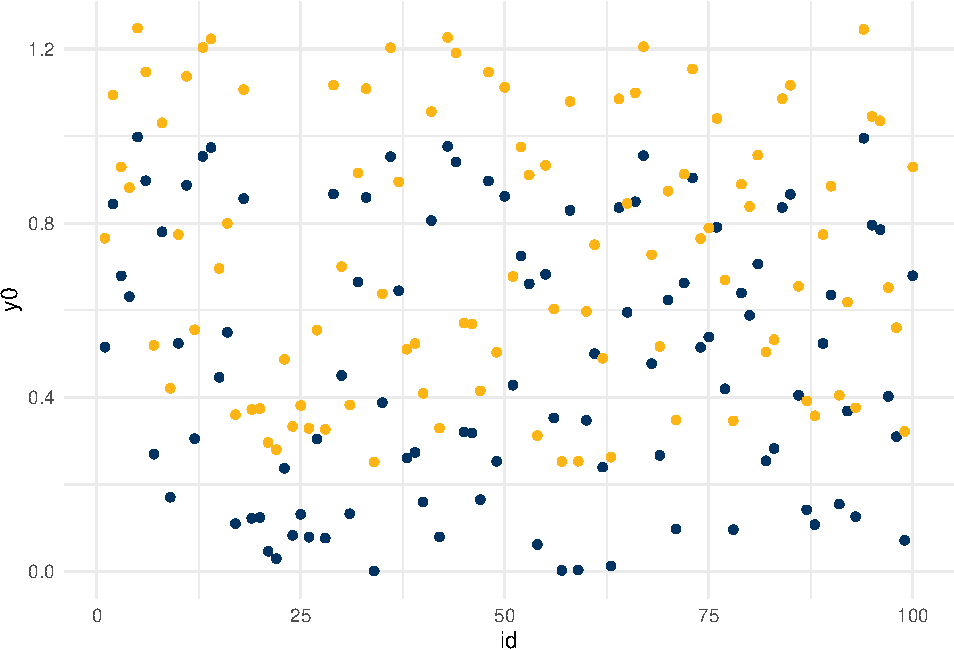
\includegraphics[keepaspectratio]{241-Live-Session_files/figure-latex/create first plot-1.pdf}}

What's actually happening in this? It might be more clear if we add arrows to this plot to show.

\begin{Shaded}
\begin{Highlighting}[]
\NormalTok{first\_plot }\SpecialCharTok{+}
  \FunctionTok{geom\_segment}\NormalTok{(}
    \FunctionTok{aes}\NormalTok{(}\AttributeTok{x =}\NormalTok{ id, }\AttributeTok{xend =}\NormalTok{ id, }\AttributeTok{y =}\NormalTok{ y0, }\AttributeTok{yend =}\NormalTok{ y1), }
    \AttributeTok{arrow =} \FunctionTok{arrow}\NormalTok{(}\AttributeTok{ends =} \StringTok{\textquotesingle{}last\textquotesingle{}}\NormalTok{, }\AttributeTok{length =} \FunctionTok{unit}\NormalTok{(}\FloatTok{0.1}\NormalTok{, }\StringTok{"inches"}\NormalTok{), }\AttributeTok{type =} \StringTok{\textquotesingle{}closed\textquotesingle{}}\NormalTok{), }
    \AttributeTok{color =} \StringTok{\textquotesingle{}grey70\textquotesingle{}}
\NormalTok{    )}
\end{Highlighting}
\end{Shaded}

\pandocbounded{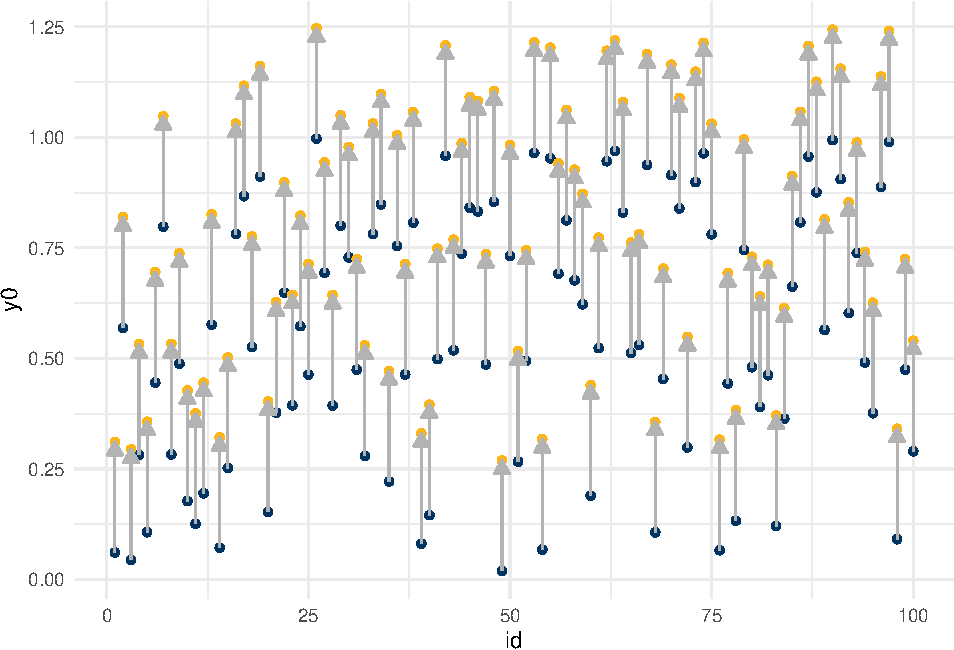
\includegraphics[keepaspectratio]{241-Live-Session_files/figure-latex/show the movement between potential outcomes-1.pdf}}

Even though these potential outcomes exist for all the units, is it possible to actually see them for all the units? How do we go about showing, and then measuring the potential outcomes to control for a set of units? How about the potential outcomes to treatment?

\begin{Shaded}
\begin{Highlighting}[]
\NormalTok{second\_plot }\OtherTok{\textless{}{-}} \FunctionTok{ggplot}\NormalTok{(}\AttributeTok{data =}\NormalTok{ d) }\SpecialCharTok{+} 
  \FunctionTok{geom\_point}\NormalTok{(}
    \FunctionTok{aes}\NormalTok{(}\AttributeTok{x =}\NormalTok{ id, }\AttributeTok{y =}\NormalTok{ y0, }\AttributeTok{size =} \DecValTok{1} \SpecialCharTok{{-}}\NormalTok{ experimental\_assignment), }
    \AttributeTok{color =}\NormalTok{ blue) }\SpecialCharTok{+} 
  \FunctionTok{geom\_point}\NormalTok{(}
    \FunctionTok{aes}\NormalTok{(}\AttributeTok{x =}\NormalTok{ id, }\AttributeTok{y =}\NormalTok{ y1, }\AttributeTok{size =} \DecValTok{0} \SpecialCharTok{+}\NormalTok{ experimental\_assignment), }
    \AttributeTok{color =}\NormalTok{ gold) }\SpecialCharTok{+} 
  \FunctionTok{labs}\NormalTok{(}
    \AttributeTok{title =} \StringTok{\textquotesingle{}Treatment and Control Assignment\textquotesingle{}}\NormalTok{, }
    \AttributeTok{size =} \StringTok{\textquotesingle{}Treatment or Control\textquotesingle{}}
\NormalTok{  )}

\NormalTok{second\_plot}
\end{Highlighting}
\end{Shaded}

\pandocbounded{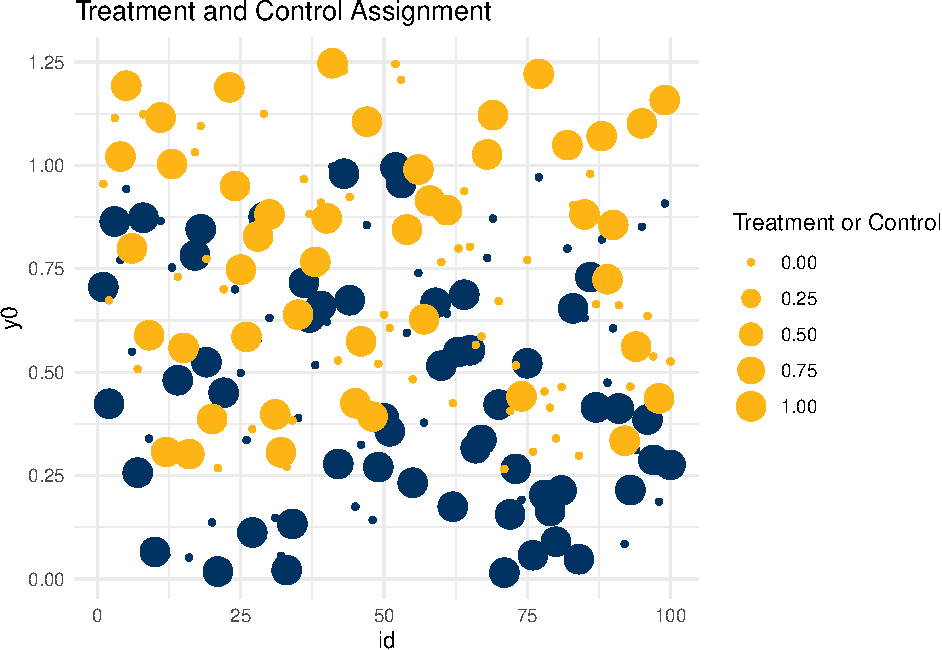
\includegraphics[keepaspectratio]{241-Live-Session_files/figure-latex/add points to plot-1.pdf}}

What are the averages of these samples that have been assigned to treatment?

\begin{Shaded}
\begin{Highlighting}[]
\NormalTok{third\_plot }\OtherTok{\textless{}{-}}\NormalTok{ second\_plot }\SpecialCharTok{+} 
  \FunctionTok{geom\_hline}\NormalTok{(}
    \AttributeTok{yintercept =} \FunctionTok{mean}\NormalTok{(d[experimental\_assignment}\SpecialCharTok{==}\DecValTok{0}\NormalTok{, y0]), }
    \AttributeTok{color =}\NormalTok{ blue, }
    \AttributeTok{linetype =} \DecValTok{2}\NormalTok{) }\SpecialCharTok{+} 
  \FunctionTok{geom\_hline}\NormalTok{(}
    \AttributeTok{yintercept =} \FunctionTok{mean}\NormalTok{(d[experimental\_assignment}\SpecialCharTok{==}\DecValTok{1}\NormalTok{, y1]), }
    \AttributeTok{color =}\NormalTok{ gold, }
    \AttributeTok{linetype =} \DecValTok{2}\NormalTok{)}
\NormalTok{third\_plot}
\end{Highlighting}
\end{Shaded}

\pandocbounded{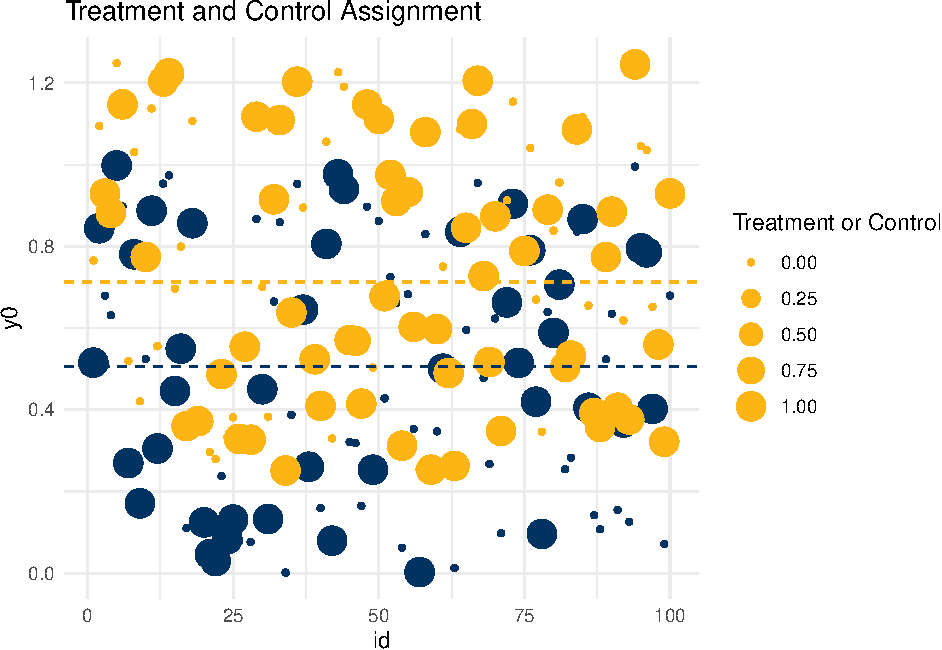
\includegraphics[keepaspectratio]{241-Live-Session_files/figure-latex/add estimates from unbiased estimator-1.pdf}}

Even though we aren't able to see it, can we reason about what the sample average would be if we could see both of an individual's potential outcome to treatment and control?

\begin{itemize}
\tightlist
\item
  Is there a guarantee that the sample should be the same as the feasible realization?
\item
  Should they be close? What property from 203 provides this guarantee?
\end{itemize}

\begin{Shaded}
\begin{Highlighting}[]
\NormalTok{third\_plot }\SpecialCharTok{+} 
  \FunctionTok{geom\_hline}\NormalTok{(}\AttributeTok{yintercept =} \FunctionTok{mean}\NormalTok{(d[, y0]), }\AttributeTok{color =}\NormalTok{ blue, }\AttributeTok{linetype =} \DecValTok{1}\NormalTok{) }\SpecialCharTok{+} 
  \FunctionTok{geom\_hline}\NormalTok{(}\AttributeTok{yintercept =} \FunctionTok{mean}\NormalTok{(d[, y1]), }\AttributeTok{color =}\NormalTok{ gold, }\AttributeTok{linetype =} \DecValTok{1}\NormalTok{)}
\end{Highlighting}
\end{Shaded}

\pandocbounded{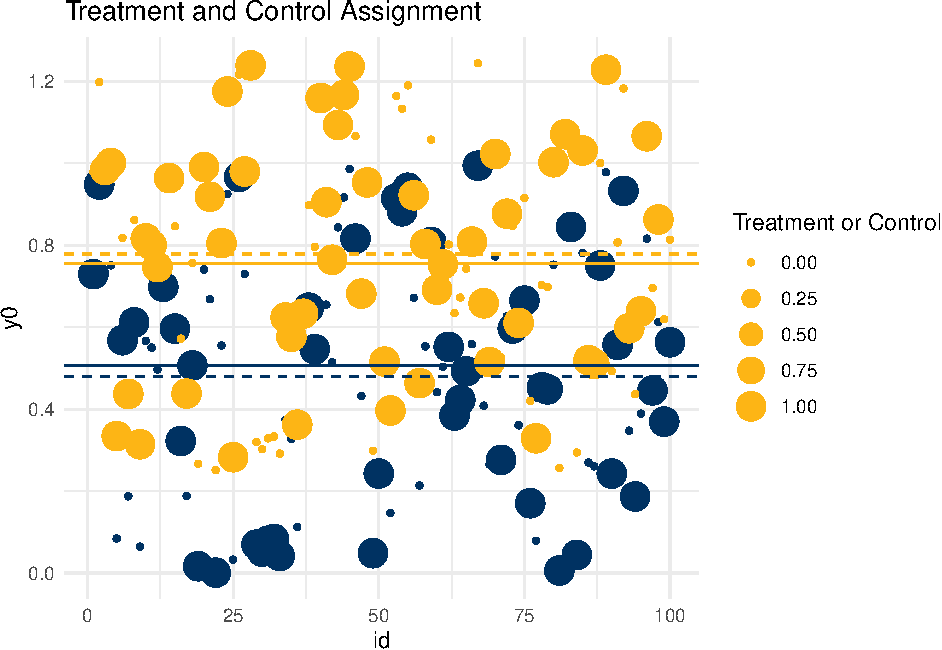
\includegraphics[keepaspectratio]{241-Live-Session_files/figure-latex/add population expected values-1.pdf}}

Put it all together, what has this little demo shown?

\subsubsection{What if there is selection?}\label{what-if-there-is-selection}

What if, rather than being assigned to treatment and control, instead individuals had been able to opt into treatment and control?

Produce only the last plot, but this time for the observational, or selected data.

\begin{Shaded}
\begin{Highlighting}[]
\NormalTok{selection\_plot }\OtherTok{\textless{}{-}} \FunctionTok{ggplot}\NormalTok{(d) }\SpecialCharTok{+} 
  \FunctionTok{geom\_point}\NormalTok{(}
    \FunctionTok{aes}\NormalTok{(}\AttributeTok{x =}\NormalTok{ id, }\AttributeTok{y =}\NormalTok{ y0, }\AttributeTok{size =} \DecValTok{1} \SpecialCharTok{{-}}\NormalTok{ observational\_selection), }
    \AttributeTok{color =}\NormalTok{ blue) }\SpecialCharTok{+} 
  \FunctionTok{geom\_point}\NormalTok{(}
    \FunctionTok{aes}\NormalTok{(}\AttributeTok{x =}\NormalTok{ id, }\AttributeTok{y =}\NormalTok{ y1, }\AttributeTok{size =} \DecValTok{0} \SpecialCharTok{+}\NormalTok{ observational\_selection), }\AttributeTok{color =}\NormalTok{ gold) }\SpecialCharTok{+} 
  \FunctionTok{geom\_hline}\NormalTok{(}
    \AttributeTok{yintercept =} \FunctionTok{mean}\NormalTok{(d[, y0]), }
    \AttributeTok{color =}\NormalTok{ blue, }
    \AttributeTok{linetype =} \DecValTok{1}\NormalTok{) }\SpecialCharTok{+} 
  \FunctionTok{geom\_hline}\NormalTok{(}
    \AttributeTok{yintercept =}\NormalTok{ d[observational\_selection }\SpecialCharTok{==} \DecValTok{0}\NormalTok{, }\FunctionTok{mean}\NormalTok{(y0)], }
    \AttributeTok{color =}\NormalTok{ blue, }
    \AttributeTok{linetype =} \DecValTok{2}\NormalTok{) }\SpecialCharTok{+} 
  \FunctionTok{geom\_hline}\NormalTok{(}
    \AttributeTok{yintercept =} \FunctionTok{mean}\NormalTok{(d[, y1]), }
    \AttributeTok{color =}\NormalTok{ gold, }
    \AttributeTok{linetype =} \DecValTok{1}\NormalTok{) }\SpecialCharTok{+}
  \FunctionTok{geom\_hline}\NormalTok{(}
    \AttributeTok{yintercept =}\NormalTok{ d[observational\_selection }\SpecialCharTok{==} \DecValTok{1}\NormalTok{, }\FunctionTok{mean}\NormalTok{(y1)], }
    \AttributeTok{color =}\NormalTok{ gold, }
    \AttributeTok{linetype =} \DecValTok{2}\NormalTok{) }\SpecialCharTok{+} 
  \FunctionTok{labs}\NormalTok{(}
    \AttributeTok{title =} \StringTok{\textquotesingle{}Observational Selection into Treatment\textquotesingle{}}\NormalTok{, }
    \AttributeTok{size =} \StringTok{\textquotesingle{}Treatment or Control\textquotesingle{}}
\NormalTok{  )}

\NormalTok{selection\_plot}
\end{Highlighting}
\end{Shaded}

\pandocbounded{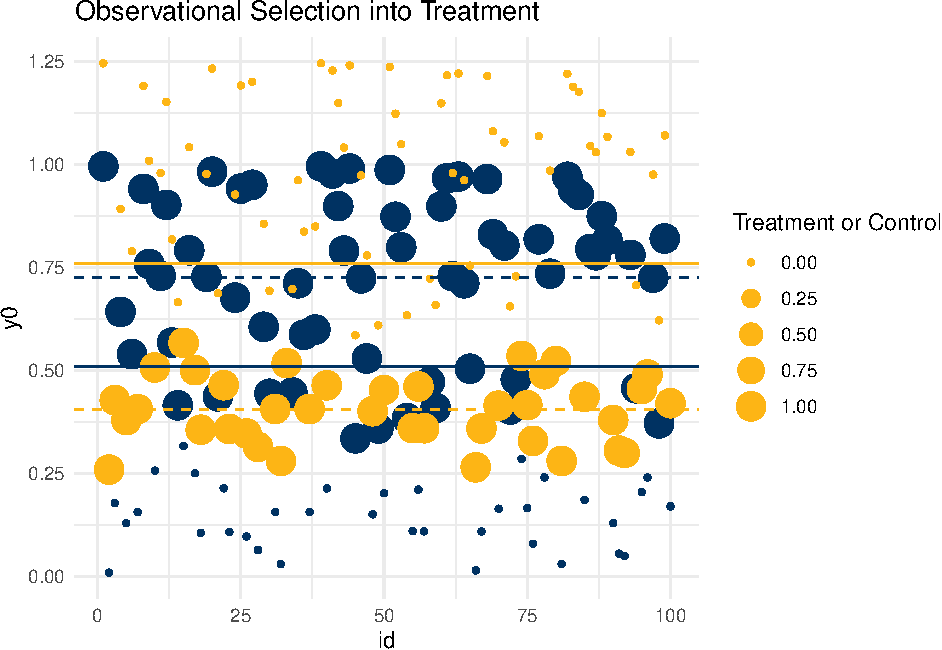
\includegraphics[keepaspectratio]{241-Live-Session_files/figure-latex/recreate plot -- for selection case-1.pdf}}

\subsection{Requirements of An Experiment}\label{requirements-of-an-experiment}

David Reiley makes the case that an experiment is something where we intervene in the world to produce knowledge. This is essentially providing a definition and making an argument that this is the correct definition. One difficulty with argument through definitions is that reasonable people can disagree because their definitions, through their lived experience, just disagree.

Here's the demonstrated proof:

\begin{quote}
Who in class is from the ``midwest'' broadly defined? Is Chicago-style pizza, pizza \emph{per se}?
Who in class is from the east coast? Is Chicago-style pizza, pizza \emph{per se}?

Try not to make deep character judgments about your classmates.
\end{quote}

Green and Gerber, in \emph{Field Experiments} make additional requirements of experiments. As they argue on page 45 of the textbook, in their view, experiments require:

\begin{enumerate}
\def\labelenumi{\arabic{enumi}.}
\tightlist
\item
  \textbf{Random Assignment}
\item
  \textbf{Excludability}
\item
  \textbf{Non-interference}
\end{enumerate}

What do each of these terms mean? Why is each necessary?

\begin{itemize}
\tightlist
\item
  Did the experiment that Daniel conducted, described in \emph{Power of Experiments} satisfy these three requirements? For any of these requirements that David's experiment did not satisfy, what are the consequences for the scientific knowledge that the experiment generated?\\
\item
  Did the Nurses Health Study, described in the async, satisfy all these three requirements? For any that this experiment did not satisfy, what are the consequences for the scientific knowledge that the experiment generated?
\end{itemize}

\subsubsection{Meta-Questions}\label{meta-questions}

\begin{itemize}
\tightlist
\item
  Can an experiment generate scientific knowledge about a causal effect, even without satisfying all of these requirements? Is it guaranteed to produce scientific knowledge about a causal effect?
\item
  What then, justifies the use of experiments to measure causal effects?
\end{itemize}

\section{Quantifying Uncertainty}\label{quantifying-uncertainty}

\subsection{Learning Objectives}\label{learning-objectives-2}

At the end of this week's live session, students will be able to

\begin{enumerate}
\def\labelenumi{\arabic{enumi}.}
\tightlist
\item
  \emph{Understand} the sharp null, and how to apply it in an argument using randomization inference.
\item
  \emph{Describe} how randomization creates uncertainty, and \emph{assess} how this uncertainty differs from that in Frequentist paradigm
\item
  \emph{Apply} the sharp null and randomization inference to data
\item
  \emph{Assess} the assumptions necessary for Frequentist inference to produce nominal coverage on confidence intervals; \emph{assess} the assumptions necessary for randomization inference to produce nominal coverage on confidence intervals; and, \emph{evaluate} which of the two approaches is appropriate given a set of data.
\item
  \emph{Describe} the concept of statistical power and what it means in the context of conducting an experiment.
\end{enumerate}

\subsection{Power of Experiments}\label{power-of-experiments}

\subsubsection{Five Key Barriers to Experimentation}\label{five-key-barriers-to-experimentation}

\emph{Power of Experiments} identifies five key barriers to experimentation in companies:

\begin{enumerate}
\def\labelenumi{\arabic{enumi}.}
\tightlist
\item
  \textbf{Not enough participants.} How can it be that even a huge, digital company (i.e.~Uber) might not have enough participants to conduct an experiment?
\item
  \textbf{Randomization can be hard to implement.} This is not to be taken lightly; because in students essays this week, nearly every experiment proposed was of the form, ``Randomly assign people to\ldots{}''. What might make it hard to randomize?
\item
  \textbf{Experiments require data to measure their impact.} This should ring of 201 conversations, but what is the concept that you would \emph{ideally} like to measure about the impact of a policy? And, what instead are you able to measure? How much conceptual slippage is there between your conceptual definition and your data?\\
\item
  \textbf{Under-appreciation of decision-makers unpredictability.} Do we actually have a theory about what people will do? How sure are we that the theory is correct?\\
\item
  \textbf{Overconfidence in our ability to guess the effect of an intervention}.
\end{enumerate}

\subsubsection{Experimental Ethics}\label{experimental-ethics}

There is a very, \emph{very} strong norm that academic researchers who conduct experiments need to pass their interventions, data collection, and procedures through a review board. This review board expects researchers will weigh the costs borne by the participants of an experimental study against the potential benefits to science from learning the results of this experiment.

In some cases, these boards determine that the costs are too high; nobody should be subject to those costs, no matter the scientific merits. In other cases, these boards will allow potentially costly actions to be taken, some that might even harm participants in the short-run. While it is quite unlikely that a review board would still approve either Milgram's or Zimbardo's infamous experiments, there are still many experiments that might harm participants.

\begin{quote}
\begin{itemize}
\tightlist
\item
  Is this OK?
\item
  What are the tradeoffs, or goals that you would like to balance in an experiment?
\end{itemize}
\end{quote}

A research team at Facebook (as your instructors if they have any juicy details about this case) was interested in the effects of their platform on its user's emotions. In pursuit of this question, they conducted an experiment -- they intentionally manipulated the environment -- to post more or fewer positive and negative posts.

\begin{quote}
\begin{itemize}
\tightlist
\item
  Is this OK?
\item
  What are the tradeoffs, or goals that you would like to balance in this experiment?
\end{itemize}
\end{quote}

\subsection{Statistical Uncertainty -- Randomization Inference Style}\label{statistical-uncertainty-randomization-inference-style}

When we are working with a sample of data, estimates produced by an estimator might change -- sometimes being higher than the \emph{true} value, other times lower than the \emph{true} value.

In Frequentist inference, we understand the variance in these estimates as \emph{sampling based variance of the sample estimator}. In this week, we present a different inferential paradigm, \textbf{Randomization Inference}.

In randomization inference, there is no uncertainty about the parameter estimate that is generated in the experiment: The estimate that we observe is the estimate that we observe. Uncertainty, instead, comes from the acknowledgment that different \emph{randomization} could have been realized, even from within the same sample.

\subsection{Stating the sharp null}\label{stating-the-sharp-null}

Suppose that you are evaluating the effect of coffee on students' alertness in class. You reason that drinking coffee will increase students' alertness in class.

\begin{figure}
\centering
\pandocbounded{
\includegraphics[keepaspectratio]{./images/damn-fine-coffee.jpeg}}
\caption{``Damn Fine Coffee.''}
\end{figure}

Continue with our idea of an experiment to evaluate if coffee produces alertness in class. Here, we are going to further develop this notional experiment into something that we might actually be able to conduct.

\begin{itemize}
\tightlist
\item
  What is the \emph{sharp null} hypothesis that is at risk in this investigation?
\item
  How, if at all, does this sharp null differ from the null hypothesis you might be more familiar with?
\item
  Is the sharp null hypothesis a concept that ever makes sense? Is the sharp null hypothesis a concept that is ever, actually, true?
\end{itemize}

\subsection{Randomization Inference}\label{randomization-inference}

\subsubsection{Stating the process of Randomization Inference}\label{stating-the-process-of-randomization-inference}

Randomization inference is a method of understanding the variability of results in an experiment that you have conducted. It specifically acknowledges several facts:

\begin{enumerate}
\def\labelenumi{\arabic{enumi}.}
\tightlist
\item
  The sample of data that you collected or used in your experiment is, quite simply, the sample of data that you collected for your experiment. There might be a larger population; there might be an infinite population; or, there might not.
\item
  The observed outcomes that you observe are, quite simply, the outcomes that you observed. There is no uncertainty about having seen these.
\item
  When the experiment assigned some units to treatment and others to the control, it revealed some outcomes, for some people. Specifically, it revealed the potential outcoems to treatment, denoted \(Y_{i}(1)\) for those who were assigned to the treatment group and the potential outcomes to control, denoted \(Y_{i}(0)\) for those who were assigned to the control group.
\item
  The experimenter chose one \emph{out of many possible} treatment assignments.
\item
  If the \emph{sharp null hypothesis} were to be true (note the subjunctive verb tense there) then, the particular revelation of potential outcomes to treatment and control are inconsequential. Despite seeing only half the data (referred to as the \textbf{Fundamental Problem of Causal Inference}) we actually posess all the data. After all, if the sharp null were true, \(Y_{Alex}(1) = Y_{Alex}(0)\), and \(Y_{David}(1) = Y_{David}(0)\), \(Y_{i}(1) = Y_{i}(0)\) for all of the \(i = {1, \dots, N}\) people who are a part of the experiment.
\end{enumerate}

\subsubsection{Questions about Randomization Inference}\label{questions-about-randomization-inference}

\begin{itemize}
\tightlist
\item
  Where does uncertainty come from in an experiment that is evaluated using randomization inference?
\item
  How is the ATE estimand defined?
\item
  What is the feasible method that we use to write down an estimator (call it \(\theta\)) for this quantity?

  \begin{itemize}
  \tightlist
  \item
    Which of the following properties does this feasible method possess?

    \begin{enumerate}
    \def\labelenumi{\alph{enumi}.}
    \tightlist
    \item
      Unbiasedness: \(E[\theta] = ATE\)
    \item
      Convergence: \(\theta \overset{p}\rightarrow ATE\), where \(\overset{p}\rightarrow\) means converges in probability
    \item
      Efficiency: The mean squared error of \(\theta\) is either (i) smaller than some other estimator, or (ii) as small is theoretically possible.
    \end{enumerate}
  \end{itemize}
\end{itemize}

\subsection{Applying Randomization Inference}\label{applying-randomization-inference}

\subsubsection{Make Data}\label{make-data}

\begin{Shaded}
\begin{Highlighting}[]
\FunctionTok{set.seed}\NormalTok{(}\DecValTok{1}\NormalTok{)}
\NormalTok{d }\OtherTok{\textless{}{-}} \FunctionTok{data.table}\NormalTok{(}
  \AttributeTok{id =} \DecValTok{1}\SpecialCharTok{:}\DecValTok{100}\NormalTok{, }
  \AttributeTok{D  =} \FunctionTok{rep}\NormalTok{(}\DecValTok{0}\SpecialCharTok{:}\DecValTok{1}\NormalTok{, }\AttributeTok{each =} \DecValTok{50}\NormalTok{), }
  \AttributeTok{Y  =} \FunctionTok{c}\NormalTok{(}\FunctionTok{rnorm}\NormalTok{(}\AttributeTok{n=}\DecValTok{50}\NormalTok{, }\AttributeTok{mean=}\DecValTok{0}\NormalTok{, }\AttributeTok{sd=}\FloatTok{2.5}\NormalTok{), }\FunctionTok{rnorm}\NormalTok{(}\AttributeTok{n=}\DecValTok{50}\NormalTok{, }\AttributeTok{mean=}\DecValTok{1}\NormalTok{, }\AttributeTok{sd=}\FloatTok{2.5}\NormalTok{))}
\NormalTok{)}
\end{Highlighting}
\end{Shaded}

\subsubsection{Plot Data}\label{plot-data}

In the following plot, are you able to assess whether there is a treatment effect simply by looking at the distributions?

\begin{Shaded}
\begin{Highlighting}[]
\FunctionTok{ggplot}\NormalTok{(d) }\SpecialCharTok{+} 
  \FunctionTok{aes}\NormalTok{(}\AttributeTok{x=}\NormalTok{Y, }\AttributeTok{fill=}\FunctionTok{as.factor}\NormalTok{(D)) }\SpecialCharTok{+} 
  \FunctionTok{geom\_density}\NormalTok{(}\AttributeTok{alpha=}\FloatTok{0.5}\NormalTok{) }\SpecialCharTok{+} 
  \FunctionTok{labs}\NormalTok{(}
    \AttributeTok{x        =} \StringTok{\textquotesingle{}Distribution of outcomes\textquotesingle{}}\NormalTok{, }
    \AttributeTok{y        =} \ConstantTok{NULL}\NormalTok{, }
    \AttributeTok{title    =} \StringTok{\textquotesingle{}Distribution of outcomes, by treatment\textquotesingle{}}\NormalTok{, }
    \AttributeTok{fill    =} \StringTok{\textquotesingle{}Treatment}\SpecialCharTok{\textbackslash{}n}\StringTok{Assignment\textquotesingle{}}\NormalTok{) }\SpecialCharTok{+} 
  \FunctionTok{scale\_fill\_manual}\NormalTok{(}
    \AttributeTok{values =} \FunctionTok{c}\NormalTok{(}\StringTok{\textquotesingle{}\#003262\textquotesingle{}}\NormalTok{, }\StringTok{\textquotesingle{}\#FDB515\textquotesingle{}}\NormalTok{)}
\NormalTok{  )}
\end{Highlighting}
\end{Shaded}

\pandocbounded{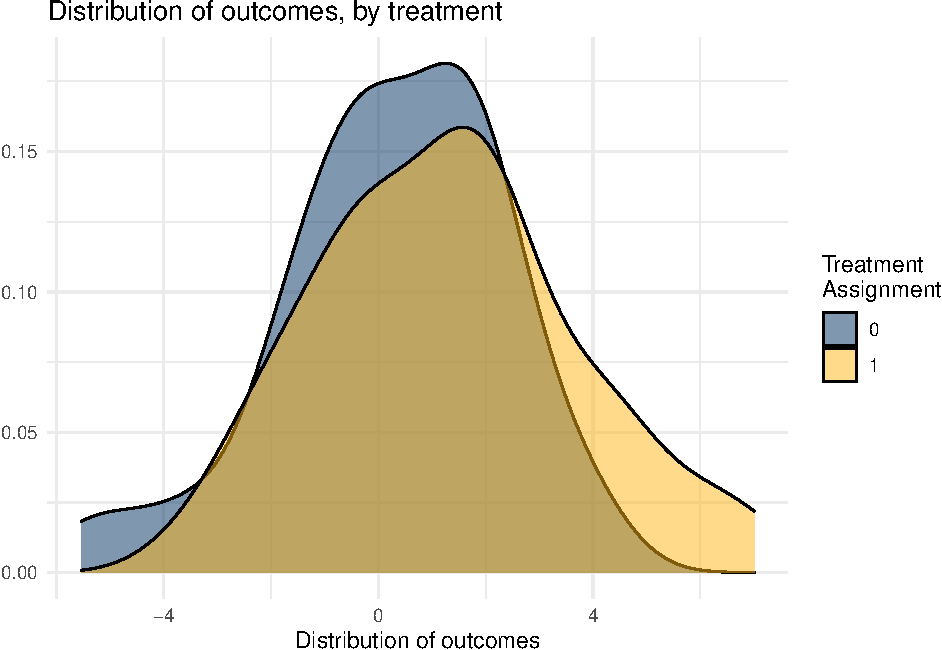
\includegraphics[keepaspectratio]{241-Live-Session_files/figure-latex/plot data-1.pdf}}

\subsubsection{Classic Test}\label{classic-test}

If you were to write a \emph{classic} test against this data, given what you know about how it was generated, what would be the classic test? What do you learn from this test, and what is the interpretation?

\begin{Shaded}
\begin{Highlighting}[]
\NormalTok{d[ , }\FunctionTok{t.test}\NormalTok{(Y }\SpecialCharTok{\textasciitilde{}}\NormalTok{ D)]}
\end{Highlighting}
\end{Shaded}

\begin{verbatim}
## 
##  Welch Two Sample t-test
## 
## data:  Y by D
## t = -2.309, df = 95.793, p-value = 0.02309
## alternative hypothesis: true difference in means between group 0 and group 1 is not equal to 0
## 95 percent confidence interval:
##  -1.9381728 -0.1462181
## sample estimates:
## mean in group 0 mean in group 1 
##       0.2511207       1.2933161
\end{verbatim}

\subsubsection{Randomization Inference Test}\label{randomization-inference-test}

Now, instead suppose that you were to conduct the randomization inference. What are the steps to the algorithm for producing a result using randomization?

\begin{enumerate}
\def\labelenumi{\arabic{enumi}.}
\tightlist
\item
  State the null hypothesis
\item
  Compute the statistic of interest using the observed data
\item
  Fill in data, under the statement of the null hypothesis
\item
  Permute the treatment assignment labels to generate a new sample of the treatment assignment vector, and then estimate the statistic of interest
\item
  Repeat the permutation and estimation (step 4) process repeatedly to sample from the randomization inference distribution of the statistic
\item
  Examine randomization inference distribution
\end{enumerate}

\begin{Shaded}
\begin{Highlighting}[]
\DocumentationTok{\#\# 1. The sharp null is that tau = 0}
\DocumentationTok{\#\# 2. Compute the statistic of interest}
\NormalTok{true\_ate }\OtherTok{\textless{}{-}}\NormalTok{ d[ , .(}\AttributeTok{group\_mean =} \FunctionTok{mean}\NormalTok{(Y)), keyby }\OtherTok{=}\NormalTok{ .(D)][ , group\_mean[D}\SpecialCharTok{==}\DecValTok{1}\NormalTok{] }\SpecialCharTok{{-}}\NormalTok{ group\_mean[D}\SpecialCharTok{==}\DecValTok{0}\NormalTok{]]}
\DocumentationTok{\#\# 3, 4, 5. Permute the treatment assignment labels and repeatedly compute the statistic of interest }
\NormalTok{ri\_distribution }\OtherTok{\textless{}{-}} \FunctionTok{replicate}\NormalTok{(}
  \AttributeTok{n=}\DecValTok{10000}\NormalTok{, }
  \AttributeTok{expr =}\NormalTok{ d[ , .(}\AttributeTok{group\_mean =} \FunctionTok{mean}\NormalTok{(Y)), }\AttributeTok{keyby =}\NormalTok{ .(}\AttributeTok{ri\_treatment =} \FunctionTok{sample}\NormalTok{(D))][ , }
\NormalTok{            group\_mean[ri\_treatment}\SpecialCharTok{==}\DecValTok{1}\NormalTok{] }\SpecialCharTok{{-}}\NormalTok{ group\_mean[ri\_treatment}\SpecialCharTok{==}\DecValTok{0}\NormalTok{]]}
\NormalTok{  )}
\CommentTok{\# 6. Examine distribution}
\FunctionTok{ggplot}\NormalTok{() }\SpecialCharTok{+} 
  \FunctionTok{geom\_density}\NormalTok{(}\FunctionTok{aes}\NormalTok{(}\AttributeTok{x=}\NormalTok{ri\_distribution), }\AttributeTok{fill =} \StringTok{\textquotesingle{}\#003262\textquotesingle{}}\NormalTok{, }\AttributeTok{alpha =} \FloatTok{0.5}\NormalTok{) }\SpecialCharTok{+} 
  \FunctionTok{geom\_vline}\NormalTok{(}\AttributeTok{xintercept =}\NormalTok{ true\_ate, }\AttributeTok{color =} \StringTok{\textquotesingle{}\#FDB515\textquotesingle{}}\NormalTok{) }\SpecialCharTok{+} 
  \FunctionTok{labs}\NormalTok{(}
    \AttributeTok{x     =} \StringTok{\textquotesingle{}Randomization Inference Distribution and Estimated ATE\textquotesingle{}}\NormalTok{, }
    \AttributeTok{y     =}  \ConstantTok{NULL}\NormalTok{, }
    \AttributeTok{title =} \StringTok{\textquotesingle{}Randomization Inference Distribution and Estimated ATE\textquotesingle{}}\NormalTok{)}
\end{Highlighting}
\end{Shaded}

\pandocbounded{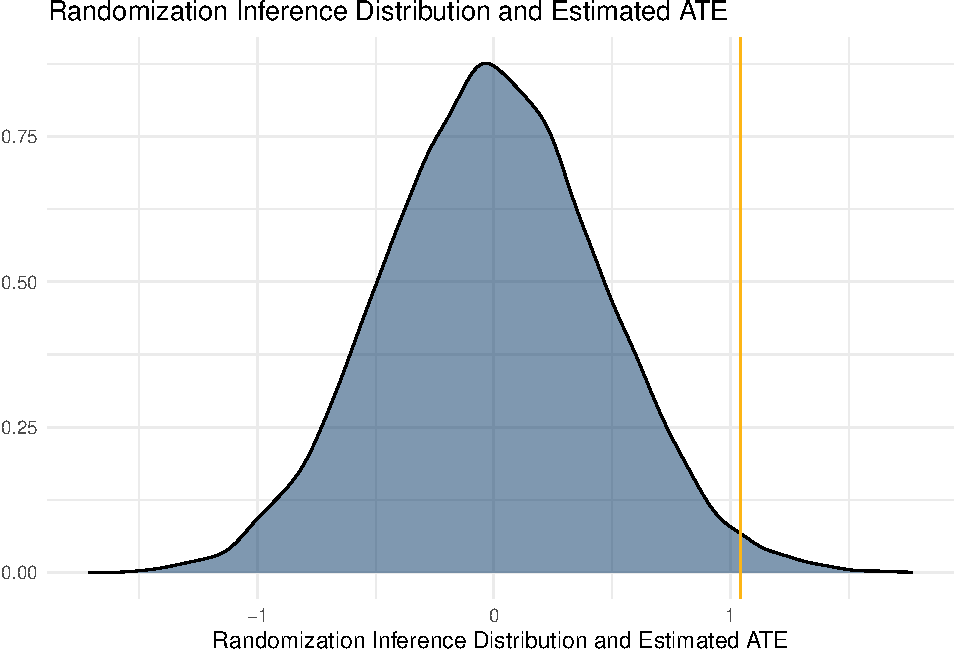
\includegraphics[keepaspectratio]{241-Live-Session_files/figure-latex/randomization inference loop-1.pdf}}

How much of the randomization inference is more extreme than the treatment effect?

\begin{Shaded}
\begin{Highlighting}[]
\NormalTok{ri\_p\_value }\OtherTok{\textless{}{-}} \FunctionTok{mean}\NormalTok{(}\FunctionTok{abs}\NormalTok{(ri\_distribution) }\SpecialCharTok{\textgreater{}} \FunctionTok{abs}\NormalTok{(true\_ate))}
\NormalTok{ri\_p\_value}
\end{Highlighting}
\end{Shaded}

\begin{verbatim}
## [1] 0.0226
\end{verbatim}

Notice that 0.023 of the randomization inference distribution is more extreme than the observed treatment effect. How does this compare to the t-test p-value that we calculated above?

\subsection{Comparing Randomization Inference and Frequentist Inference}\label{comparing-randomization-inference-and-frequentist-inference}

If both Randomization Inference and Frequentist Inference produce similar p-values, what is utility in learning another set of methods for communicating estimator-based uncertainty?

What are the requirements (frequently referred to as ``assumptions'') that are necessary for the Frequentist paradigm to provide guarantees? What happens if these guarantees are not, in fact, satisfied or true in the data generating process? How do you react, respond, or address those problems?

\begin{itemize}
\tightlist
\item
  If data is not sampled \emph{iid}, is it sufficient to simply note that limitation (frequently referred to as an ``assumption violation'') and report whatever p-value you report?
\item
  How affected is this p-value by the violation? How do you know this?
\item
  What does it mean for the p-value to be affected by this violation? (\emph{Recall that a p-value is just a random variable that is produced through a series of summarizing transformations and then a comparison against a reference distribution.})
\end{itemize}

\subsubsection{Donations to a political campaign}\label{donations-to-a-political-campaign}

In \emph{Field Experiments} Green and Gerber provide some useful (hypothetical) data about donations to a political campaign. The data is defined in the following way, \(D\) is an indicator for whether the potential donor is assigned to treatment or control, and \(Y\) is the outcome of how much the potential donor actually gave.

Let us provide a little bit more back story, that is necessary for the example to work, fully. Suppose that a progressive political candidate was hosting a fundraiser in Berkeley and has to make a choice about what to serve the attendees at the fundraiser.

In the \(D = 0\) group, suppose that the candidate elects to serve a hippie-vegetarian staple, tofu sauteed in Bragg's liquid aminos. (It \emph{is} Berkeley after all.) In the \(D=1\) group, suppose that the candidate decides to be a little more, well, progressive in their vegetarian food offerings and instead serves Gado-Gado from Katzen's \emph{The Enchanted Broccoli Forest}. (Still Berkeley\ldots{} .)

After dinner, and the requisite drum-circle, attendees to this shin-dig are asked to donate to the candidates re-election efforts. Every attendee is expected to contribute something -- social norms rule out failing to donate when the collection plate is passed -- but the amount donated is at the discretion of the attendee.

\begin{Shaded}
\begin{Highlighting}[]
\NormalTok{d }\OtherTok{\textless{}{-}} \FunctionTok{data.table}\NormalTok{(}
  \AttributeTok{id =} \DecValTok{1}\SpecialCharTok{:}\DecValTok{20}\NormalTok{, }
  \AttributeTok{D  =} \FunctionTok{rep}\NormalTok{(}\DecValTok{0}\SpecialCharTok{:}\DecValTok{1}\NormalTok{, }\AttributeTok{each =} \DecValTok{10}\NormalTok{), }
  \AttributeTok{Y =} \FunctionTok{c}\NormalTok{(}\DecValTok{500}\NormalTok{, }\DecValTok{100}\NormalTok{, }\DecValTok{100}\NormalTok{, }\DecValTok{50}\NormalTok{, }\DecValTok{25}\NormalTok{, }\DecValTok{25}\NormalTok{, }\DecValTok{0}\NormalTok{, }\DecValTok{0}\NormalTok{, }\DecValTok{0}\NormalTok{, }\DecValTok{0}\NormalTok{, }\DocumentationTok{\#\# tofu diners}
        \DecValTok{25}\NormalTok{,  }\DecValTok{20}\NormalTok{,  }\DecValTok{15}\NormalTok{,  }\DecValTok{15}\NormalTok{, }\DecValTok{10}\NormalTok{, }\DecValTok{5}\NormalTok{,  }\DecValTok{5}\NormalTok{, }\DecValTok{0}\NormalTok{, }\DecValTok{0}\NormalTok{, }\DecValTok{0}\NormalTok{)  }\DocumentationTok{\#\# gado gado diners}
\NormalTok{)}
\end{Highlighting}
\end{Shaded}

\begin{enumerate}
\def\labelenumi{\arabic{enumi}.}
\tightlist
\item
  With this data, conduct a \texttt{t.test} to assess whether the choice of dinner affects the amount donated to the campaign. What is your null-hypothesis (be specific), what is your rejection criteria, and do you reject or fail to reject this null hypothesis under the t-test framework.
\end{enumerate}

\begin{Shaded}
\begin{Highlighting}[]
\DocumentationTok{\#\# Null Hypothesis: }
\DocumentationTok{\#\# Rejection Criteria: }

\DocumentationTok{\#\# Conduct the Test Here: }

\DocumentationTok{\#\# Conclusion: }
\end{Highlighting}
\end{Shaded}

\begin{enumerate}
\def\labelenumi{\arabic{enumi}.}
\setcounter{enumi}{1}
\tightlist
\item
  With this data, use randomization inference to assess whether the choice of dinner affects the amount donated to the campaign. What is your null-hypothesis (be specific), what is your rejection criteria, and do you reject or fail to reject this null hypothesis under the t-test framework.
\end{enumerate}

\begin{Shaded}
\begin{Highlighting}[]
\DocumentationTok{\#\# Null Hypothesis: }
\DocumentationTok{\#\# Rejection Criteria: }

\DocumentationTok{\#\# Conduct the Test Here:}

\DocumentationTok{\#\# Conclusion}
\end{Highlighting}
\end{Shaded}

\begin{enumerate}
\def\labelenumi{\arabic{enumi}.}
\item
  Characterize the distribution of the sharp-null distribution of treatment effects. Talk about what, if anything, is notable about it, and what components of the data might be leading to any patterns that you note.
\item
  How many of the randomization inference loops are larger than the treatment effect that you calculated? How would you use this statement to construct a one-sided test, and an associated p-value?
\item
  How many of the randomization inference loops are \emph{more extreme} (:metal:) than the treatment effect that you calculated? How would you use this statement to construct a two-sided test, and an associated p-value?
\item
  Compare the two-sided p-value against the p-value that you generate from a two-tailed t-test. If these p-values are the same, would this be a positive or a negative characteristic of randomization inference? If these p-values are different, why would they be different? Don't go looking all over hill-and-dale for the call for a t-test, it is at \texttt{t.test}.
\item
  Which of the two of these inferential methods do you prefer, randomization inference or a t-test, and why? Ease of use is not an acceptable answer.
\end{enumerate}

\subsection{Statistical Power}\label{statistical-power}

\begin{itemize}
\tightlist
\item
  What is statistical power?
\item
  Why is it particularly relevant to consider statistical power when you are thinking about conducting an experiment?

  \begin{itemize}
  \tightlist
  \item
    What would happen if you were to conduct an experiment that has only an achieved power of 0.1?
  \item
    What would you learn if you were to fail to reject the sharp-null hypothesis?
  \item
    What would you learn if you were to reject the sharp-null hypothesis?
  \end{itemize}
\end{itemize}

\begin{Shaded}
\begin{Highlighting}[]
\NormalTok{make\_data }\OtherTok{\textless{}{-}} \ControlFlowTok{function}\NormalTok{(}
  \AttributeTok{sample\_size                       =} \DecValTok{100}\NormalTok{,}
  \AttributeTok{potential\_outcome\_to\_control\_mean =} \DecValTok{10}\NormalTok{,}
  \AttributeTok{potential\_outcome\_to\_control\_sd   =} \DecValTok{2}\NormalTok{, }
  \AttributeTok{treatment\_effect                  =} \DecValTok{1}\NormalTok{, }
  \AttributeTok{sd\_treatment                      =} \DecValTok{2}\NormalTok{) \{ }
  \DocumentationTok{\#\# this is a function to make data to simulate the power of a test}
  
\NormalTok{  \}}
  
\NormalTok{test\_data }\OtherTok{\textless{}{-}} \ControlFlowTok{function}\NormalTok{(data, treatment\_indicator, outcome) \{}
  
\NormalTok{\}}
 
\DocumentationTok{\#\# p\_values \textless{}{-} replicate(n = 1000) }
\end{Highlighting}
\end{Shaded}

\section{Blocking and Clustering}\label{blocking-and-clustering}

When assigning treatment to units, unless there are restrictions created by the researcher, any of the treatment assignment vectors are equally probable. Blocking and clustering are ways of restricting the treatment assignments to a subset of the whole schedule of possibilities.

\emph{Blocking} is a method of creating ``blocks'', or groups, of units that are similar along one or more dimensions and then creating a full random assignment within each of those similar groups. Through careful design, blocking can generate power or nuance for an experiment without any extra marginal costs for paying for additional units of treatment.

\emph{Clustering} is a circumstance that arises from a state of the world that \emph{requires} you to assign several similar units to the same condition, be it treatment or control. Through careful design, clustering might not hamper the power of an experiment; though realizing the necessity of a clustered design is typically met with the following statement, ``@\#\$\%, we've got to cluster.''

\subsection{Learning Objectives}\label{learning-objectives-3}

At the end of this week, student will be able to

\begin{enumerate}
\def\labelenumi{\arabic{enumi}.}
\tightlist
\item
  \textbf{Recognize} when there is the potential to block random assign in their experiment, and \textbf{remember} why block random assignment beneficial.
\item
  \textbf{Recognize} when they are required to cluster random assign -- either due to a pragmatic (i.e.~real-world) limitation, or to avoid violating the requirement that units not interfere with one another -- and \textbf{identify} ways that they can mitigate the reduction-in-power that arises from the need to cluster.
\item
  \textbf{Distinguish} between the circumstances that lead to blocking and clustering.
\item
  \textbf{Analyze} both blocked and clustered experiments using the appropriate test, and generating statements of certainty and uncertainty using \emph{randomization inference}.
\end{enumerate}

\subsection{Setting terms: Blocking}\label{setting-terms-blocking}

\begin{itemize}
\tightlist
\item
  What does it mean to block randomize?
\item
  Does the elimination of some randomization mean that the randomization is not longer, well, random?
\item
  Relative to when treatment is administered, when are we able to block? Why are we not able to block after we've assigned treatment?
\end{itemize}

\subsection{Math: Block random assignment}\label{math-block-random-assignment}

In equation 3.6 (on page 61) of \emph{Field Experiments} Green and Gerber write,

\[ 
  \widehat{SE} = \sqrt{\frac{\widehat{Var}(Y_{i}(0))}{N-m} + \frac{\widehat{Var}(Y_{i}(1))}{m}}
\]

When we block randomize, we're essentially creating smaller groups of units and producing an estimate of the variance within each of those smaller groups of units.

How do the authors arrive at the following formula for a block randomized standard error?

\[ 
  \widehat{SE}(\widehat{ATE}_{blocked}) = \sqrt{\sum_{j=1}^{J}\left(\frac{N_{j}}{N}\right)^2 * \widehat{SE}^2(\widehat{ATE}_{j})}
\]

\begin{itemize}
\tightlist
\item
  Specifically, why are we squaring the scaling parameter \(\frac{N_{j}}{N}\)?
\item
  If you look at this summation, what has to happen to the variance within the groups, relative to the size of the groups, in order for blocking to actually increase power?
\item
  Is it possible that you block, without increasing power, even if the blocking variable is actually useful?
\end{itemize}

Green and Gerber, in equation 3.10, write that the overall \(ATE\) of the population is:

\[ 
  ATE = \sum_{j=1}^{J} \frac{N_{j}}{N} ATE_{j}
\]

\begin{itemize}
\item
  What does this equation ``feel like''? Does that seem reasonable? Why or why not?
\item
  Why might it be a good idea to have different rates of assignment to treatment within different blocks? Consider the following example:

  \begin{itemize}
  \tightlist
  \item
    Suppose that you are looking at an experiment among your whole user base, and you are considering changing the ``check out flow'' (we have not idea what that might mean either\ldots) for this group.
  \item
    Some of the users are \emph{really} likely to purchase, while others are very unlikely to purchase.
  \item
    Does it make sense to block randomize based on this prior purchase history?
  \item
    Are there any, reasonable business reasons to not make the treatment assignments be 50\% treatment and 50\% control in both of the populations?
  \item
    What would happen if you randomized 10\% of the ``high value'' customers into treatment and 50\% of the low value customers into treatment. But, then you forget (or lost) that table of whether they were ``high'' or ``low'' value customers.
  \item
    \emph{What would be the consequence to your treatment effect estimate?}
  \end{itemize}
\end{itemize}

\subsection{Intuition: Block Random Assignment}\label{intuition-block-random-assignment}

To discuss the idea of blocking, consider the working example that David and David present in the async lectures:

\begin{quote}
Eating too much tofu (aka the \emph{Berkeley diet}) might increase decrease one's brain function, leading to decreased performance on cognitive tests, lower brain weight, and cause ventrical enlargment of the brain.

Don't ask your instructors what any of that medical jargon might mean. It isn't our field! But, these are real claims made by a group of researchers in an observational nutrition study titled ``Brain Aging and Midlife Tofu Consumption.''
\end{quote}

\begin{figure}
\centering
\pandocbounded{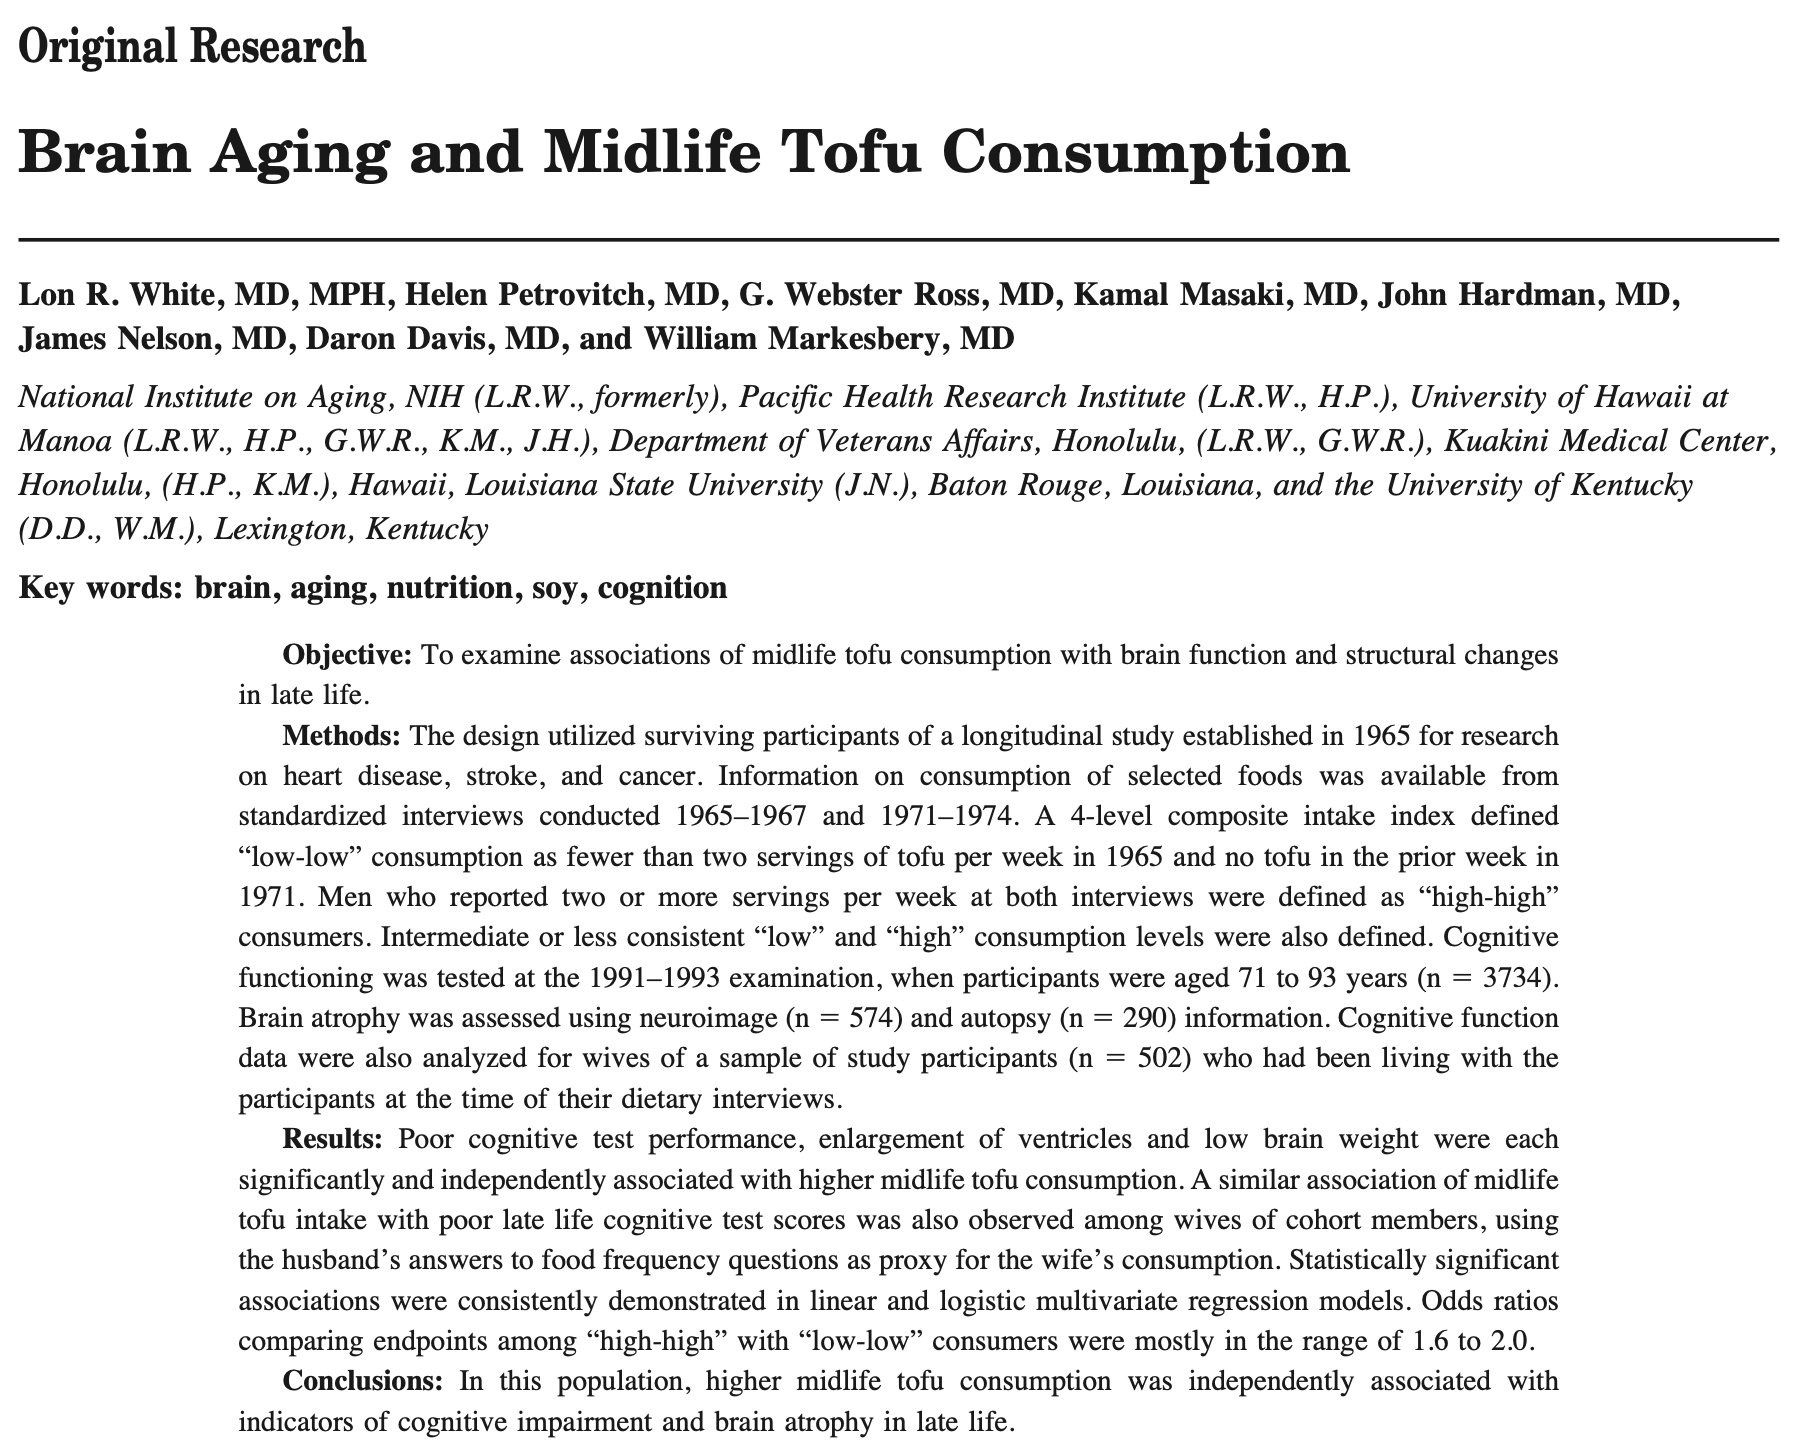
\includegraphics[keepaspectratio]{./images/this_is_your_brain_on_tofu_abstract.png}}
\caption{this is your brain on tofu}
\end{figure}

Suppose that, motivated by your distaste for bunk, casual causal claims about diet, and taste for tofu, you decide to conduct a real experiment among your friends, families, and classmates to determine the actual impacts of tofu on diet.

\begin{Shaded}
\begin{Highlighting}[]
\FunctionTok{set.seed}\NormalTok{(}\DecValTok{1414}\NormalTok{)}

\NormalTok{sim\_normal\_study }\OtherTok{\textless{}{-}} \ControlFlowTok{function}\NormalTok{(}\AttributeTok{treatment\_effect=}\DecValTok{0}\NormalTok{) \{}
  \DocumentationTok{\#\# this function will create a "world" to analyze using an experiment, }
  \DocumentationTok{\#\# then, it will estimate the ate within that world }
  \DocumentationTok{\#\# it returns the ate and the number of women who are in treatment }
  
  \FunctionTok{require}\NormalTok{(data.table)}
  
\NormalTok{  d }\OtherTok{\textless{}{-}} \FunctionTok{data.table}\NormalTok{(}
      \AttributeTok{group        =} \FunctionTok{rep}\NormalTok{(}\FunctionTok{c}\NormalTok{(}\StringTok{\textquotesingle{}M\textquotesingle{}}\NormalTok{, }\StringTok{\textquotesingle{}F\textquotesingle{}}\NormalTok{), }\AttributeTok{each =} \DecValTok{20}\NormalTok{), }
      \AttributeTok{po\_control   =} \FunctionTok{c}\NormalTok{(}\DecValTok{1}\SpecialCharTok{:}\DecValTok{20}\NormalTok{, }\DecValTok{81}\SpecialCharTok{:}\DecValTok{100}\NormalTok{), }
        \DocumentationTok{\#\# treatment\_effect = 0 {-}{-}\textgreater{} sharp null is true}
      \AttributeTok{po\_treatment =} \FunctionTok{c}\NormalTok{(}\DecValTok{1}\SpecialCharTok{:}\DecValTok{20}\NormalTok{, }\DecValTok{81}\SpecialCharTok{:}\DecValTok{100}\NormalTok{) }\SpecialCharTok{+}\NormalTok{ treatment\_effect, }
      \AttributeTok{treatment =} \FunctionTok{sample}\NormalTok{(}\DecValTok{1}\SpecialCharTok{:}\DecValTok{0}\NormalTok{, }\AttributeTok{size =} \DecValTok{40}\NormalTok{, }\AttributeTok{replace =} \ConstantTok{TRUE}\NormalTok{))[ , }\DocumentationTok{\#\# notice we\textquotesingle{}re now assigning}
\NormalTok{      outcomes }\SpecialCharTok{:=}\NormalTok{ po\_treatment }\SpecialCharTok{*}\NormalTok{ treatment }\SpecialCharTok{+}\NormalTok{ po\_control }\SpecialCharTok{*}\NormalTok{ (}\DecValTok{1} \SpecialCharTok{{-}}\NormalTok{ treatment)]}

\NormalTok{  ate }\OtherTok{\textless{}{-}}\NormalTok{ d[ , }\FunctionTok{mean}\NormalTok{(outcomes[treatment }\SpecialCharTok{==} \DecValTok{1}\NormalTok{]) }\SpecialCharTok{{-}} \FunctionTok{mean}\NormalTok{(outcomes[treatment }\SpecialCharTok{==} \DecValTok{0}\NormalTok{])]}
\NormalTok{  n\_women\_treatment }\OtherTok{=}\NormalTok{ d[treatment }\SpecialCharTok{==} \DecValTok{1} \SpecialCharTok{\&}\NormalTok{ group }\SpecialCharTok{==} \StringTok{\textquotesingle{}F\textquotesingle{}}\NormalTok{, .N]}

  \FunctionTok{return}\NormalTok{(}\FunctionTok{list}\NormalTok{(}
    \AttributeTok{data =}\NormalTok{ d,}
    \AttributeTok{ate =}\NormalTok{ ate, }
    \AttributeTok{n\_women\_treatment =}\NormalTok{ n\_women\_treatment}
\NormalTok{    ))}
\NormalTok{\}}
\end{Highlighting}
\end{Shaded}

\subsection{With this data, what does the distribution of outcomes look like?}\label{with-this-data-what-does-the-distribution-of-outcomes-look-like}

\begin{Shaded}
\begin{Highlighting}[]
\NormalTok{experiment\_one }\OtherTok{\textless{}{-}} \FunctionTok{sim\_normal\_study}\NormalTok{(}\AttributeTok{treatment\_effect =} \DecValTok{0}\NormalTok{)}
\NormalTok{experiment\_two }\OtherTok{\textless{}{-}} \FunctionTok{sim\_normal\_study}\NormalTok{(}\AttributeTok{treatment\_effect =} \DecValTok{10}\NormalTok{)}
\end{Highlighting}
\end{Shaded}

\begin{Shaded}
\begin{Highlighting}[]
\NormalTok{experiment\_one\_plot }\OtherTok{\textless{}{-}} \FunctionTok{ggplot}\NormalTok{(}\AttributeTok{data =}\NormalTok{ experiment\_one}\SpecialCharTok{$}\NormalTok{data) }\SpecialCharTok{+} 
  \FunctionTok{aes}\NormalTok{(}\AttributeTok{x =}\NormalTok{ outcomes, }\AttributeTok{fill =} \FunctionTok{factor}\NormalTok{(treatment), }\AttributeTok{linetype =}\NormalTok{ group) }\SpecialCharTok{+} 
  \FunctionTok{geom\_density}\NormalTok{(}\AttributeTok{alpha =} \FloatTok{0.5}\NormalTok{) }\SpecialCharTok{+} 
  \FunctionTok{labs}\NormalTok{(}\AttributeTok{title =} \StringTok{\textquotesingle{}No effect\textquotesingle{}}
\NormalTok{  )}
\NormalTok{experiment\_two\_plot }\OtherTok{\textless{}{-}} \FunctionTok{ggplot}\NormalTok{(}\AttributeTok{data =}\NormalTok{ experiment\_two}\SpecialCharTok{$}\NormalTok{data) }\SpecialCharTok{+} 
  \FunctionTok{aes}\NormalTok{(}\AttributeTok{x =}\NormalTok{ outcomes, }\AttributeTok{fill =} \FunctionTok{factor}\NormalTok{(treatment), }\AttributeTok{linetype =}\NormalTok{ group) }\SpecialCharTok{+} 
  \FunctionTok{geom\_density}\NormalTok{(}\AttributeTok{alpha =} \FloatTok{0.5}\NormalTok{) }\SpecialCharTok{+} 
  \FunctionTok{labs}\NormalTok{(}\AttributeTok{title =} \StringTok{\textquotesingle{}Ten unit effect\textquotesingle{}}
\NormalTok{  )}

\NormalTok{(experiment\_one\_plot }\SpecialCharTok{/}\NormalTok{ experiment\_two\_plot) }\SpecialCharTok{+} 
  \FunctionTok{plot\_annotation}\NormalTok{(}\AttributeTok{title =} \StringTok{\textquotesingle{}Measured Distribution of Estrogen, by Group\textquotesingle{}}\NormalTok{) }\SpecialCharTok{+} 
  \FunctionTok{plot\_layout}\NormalTok{(}\AttributeTok{guides =} \StringTok{\textquotesingle{}collect\textquotesingle{}}\NormalTok{)}
\end{Highlighting}
\end{Shaded}

\pandocbounded{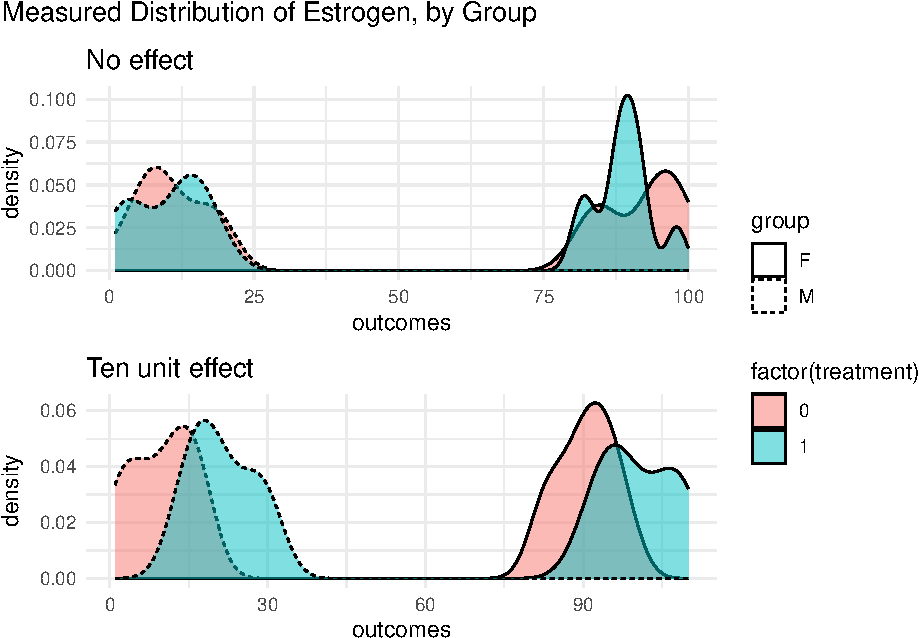
\includegraphics[keepaspectratio]{241-Live-Session_files/figure-latex/unnamed-chunk-1-1.pdf}}

In these two different cases -- where there is no treatment effect on top, and when there is a large treatment effect on bottom -- what are the group means? Where would they be on these plots?

Consider the formula for the SE\_\{ATE\}.

\[
  SE(\tau) \approx \sqrt{\frac{V[\tau]}{N}}
\]

The important parts to consider for this discussion (despite being not a full statement of the SE) is that the standard error of the difference of group averages is a ratio of the underlying variance of the treatment effect, divided by the number of observations in that group.

\[
  \begin{aligned}
  SE[\tau] & \approx \sqrt{\frac{V[Y(1)]}{n_{1}} + \frac{V[Y(0)]}{n_{0}}} \\ 
           & \approx \sqrt{\frac{E[\left(Y(1) - E[Y(1)]\right)^2]}{n_{1}} + \frac{E[\left(Y(0) - E[Y(0)]\right)^2]}{n_{0}}}
  \end{aligned}
\]

\begin{itemize}
\tightlist
\item
  When you examine the plot above, what are the expected values of the treatment and control groups?
\item
  What does the expected value of the square of the deviations look like on this plot?
\end{itemize}

\subsection{Technical Benefits of Blocking}\label{technical-benefits-of-blocking}

How how does breaking this population into two smaller groups create a reduction in the calculated standard error that you observe from an experiment?

\begin{itemize}
\tightlist
\item
  What is (draw) the conditional expectation among the \texttt{M} group and the \texttt{F} group.
\item
  What is (draw) the conditional variance among the \texttt{M} group and the \texttt{F} group.
\item
  How has this change produced a reduction in the overall variance?
\end{itemize}

\begin{Shaded}
\begin{Highlighting}[]
\NormalTok{experiment\_one\_plot }\OtherTok{\textless{}{-}} \FunctionTok{ggplot}\NormalTok{(}\AttributeTok{data =}\NormalTok{ experiment\_one}\SpecialCharTok{$}\NormalTok{data) }\SpecialCharTok{+} 
  \FunctionTok{aes}\NormalTok{(}\AttributeTok{x =}\NormalTok{ outcomes, }\AttributeTok{fill =} \FunctionTok{factor}\NormalTok{(treatment), }\AttributeTok{linetype =}\NormalTok{ group) }\SpecialCharTok{+} 
  \FunctionTok{geom\_density}\NormalTok{(}\AttributeTok{alpha =} \FloatTok{0.5}\NormalTok{) }\SpecialCharTok{+} 
  \FunctionTok{labs}\NormalTok{(}\AttributeTok{title =} \StringTok{\textquotesingle{}No effect\textquotesingle{}}
\NormalTok{  )}
\NormalTok{experiment\_two\_plot }\OtherTok{\textless{}{-}} \FunctionTok{ggplot}\NormalTok{(}\AttributeTok{data =}\NormalTok{ experiment\_two}\SpecialCharTok{$}\NormalTok{data) }\SpecialCharTok{+} 
  \FunctionTok{aes}\NormalTok{(}\AttributeTok{x =}\NormalTok{ outcomes, }\AttributeTok{fill =} \FunctionTok{factor}\NormalTok{(treatment), }\AttributeTok{linetype =}\NormalTok{ group) }\SpecialCharTok{+} 
  \FunctionTok{geom\_density}\NormalTok{(}\AttributeTok{alpha =} \FloatTok{0.5}\NormalTok{) }\SpecialCharTok{+} 
  \FunctionTok{labs}\NormalTok{(}\AttributeTok{title =} \StringTok{\textquotesingle{}Ten unit effect\textquotesingle{}}
\NormalTok{  )}

\NormalTok{(experiment\_one\_plot }\SpecialCharTok{/}\NormalTok{ experiment\_two\_plot) }\SpecialCharTok{+} 
  \FunctionTok{plot\_annotation}\NormalTok{(}\AttributeTok{title =} \StringTok{\textquotesingle{}Measured Distribution of Estrogen, by Group\textquotesingle{}}\NormalTok{) }\SpecialCharTok{+} 
  \FunctionTok{plot\_layout}\NormalTok{(}\AttributeTok{guides =} \StringTok{\textquotesingle{}collect\textquotesingle{}}\NormalTok{)}
\end{Highlighting}
\end{Shaded}

\pandocbounded{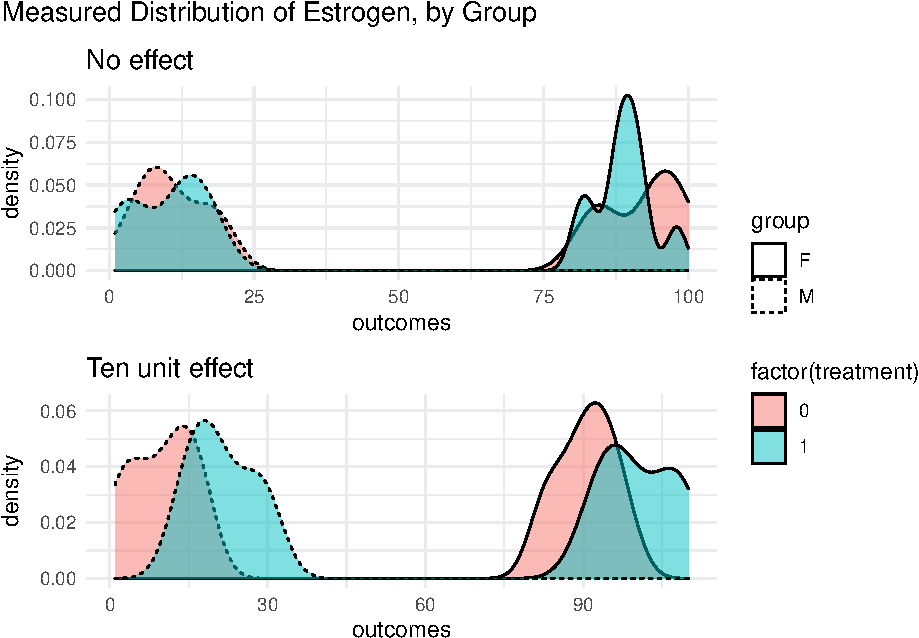
\includegraphics[keepaspectratio]{241-Live-Session_files/figure-latex/unnamed-chunk-2-1.pdf}}

\subsection{How should we block randomize?}\label{how-should-we-block-randomize}

Let's take several discussion points, in order:

\subsubsection{What makes a useful feature? (part 1)}\label{what-makes-a-useful-feature-part-1}

\begin{itemize}
\item
  When we are considering a block randomization to improve the \emph{power} of a test, what about a feature makes it a useful blocking feature? (For instructors, probably don't read each of these, but try to get the discussion to address them.)

  \begin{itemize}
  \tightlist
  \item
    Does a good blocking feature have to be associated with the treatment?
  \item
    Does a good blocking feature have to be associated with potential outcomes?
  \item
    Does a good blocking feature have to have a causal effect on the measured outcomes?
  \end{itemize}
\item
  Suppose that have two possible features that you could use to block in the estrogen experiment. Either, you can block randomize using:

  \begin{enumerate}
  \def\labelenumi{(\alph{enumi})}
  \tightlist
  \item
    blood-serum levels of estrogen, measured a week before the experiment begins; or (
  \end{enumerate}

  \begin{enumerate}
  \def\labelenumi{\alph{enumi})}
  \setcounter{enumi}{1}
  \tightlist
  \item
    ``stated form'' sex (i.e.~female, male, nonbinary).
  \end{enumerate}
\end{itemize}

\subsubsection{What makes a useful feature (part 2)}\label{what-makes-a-useful-feature-part-2}

\begin{itemize}
\item
  In the async, and to this point in this live session, we have spoken only about features that are categorical for blocking.
\item
  Is it possible to block on a continuous feature?

  \begin{itemize}
  \tightlist
  \item
    What if it were measured very, very precisely, so every unit had a unique value on a continuous variable?
  \item
    If you \emph{could} develop a method of blocking on a continuous variable, what might be the benefits?
  \end{itemize}
\end{itemize}

\subsubsection{Strategies of blocking}\label{strategies-of-blocking}

\begin{itemize}
\item
  If there is a benefit of creating two mini-experiments through blocking -- as you have proposed in the code above -- could there be a benefit to creating a third mini-experiment through blocking? What about a fourth? Is there a limit that you run into?

  \begin{itemize}
  \tightlist
  \item
    What is the most blocks that you can produce in an experiment?
  \item
    Or, alternatively, what is the smallest size block that you can produce in an experiment?
  \item
    Is there a reason to take this strategy?
  \item
    What if you created many blocks, but with a noisy blocking feature. Would this work well?
  \item
    What if you created many blocks, but with a very precise blocking feature. Would this work well?
  \end{itemize}
\item
  To this point, we have discussed blocking on only a single variable. Is it possible to block on more than one variable at a time?

  \begin{itemize}
  \tightlist
  \item
    If you have already blocked on one variable, what are the characteristics that are useful for the next variable that you consider blocking on?
  \item
    For example, suppose that you have already blocked the tofu experiment on experimental units' stated-form sex. Would it be useful to then block based on wearing glasses, or hair length, or blood-serum estrogen? Why or why not?
  \end{itemize}
\end{itemize}

\subsection{Clustering}\label{clustering}

\begin{itemize}
\tightlist
\item
  What are the circumstances in the world that make it necessary to cluster random assign?
\item
  Are these circumstances academic? Or, are there actually examples of where this might come into play?

  \begin{itemize}
  \tightlist
  \item
    Consider the ride sharing example that we read about in \emph{Power of Experiments}. What would happen if we gave some people really low prices to get into a rideshare, while we gave other people really high prices? What if they are standing next to eachother at the airport? What if one is at an airport in Oakland, while the other is at SFO?
  \end{itemize}
\end{itemize}

\subsection{Blocking or Clustering?}\label{blocking-or-clustering}

\subsubsection{Let is snow!}\label{let-is-snow}

Suppose we want to measure the effect of snowplowing on local retail activity. We design an experiment that plows some locations but not others. Which of the following do you prefer? Explain the relative advantages and disadvantages of each option.

\begin{itemize}
\tightlist
\item
  On a given street, we randomly assign which businesses we plow in front of.
\item
  We randomly assign which streets to plow and which streets not to plow.
\item
  We randomly assign which neighborhoods to plow and which neighborhoods not to plow.
\item
  Do the differences above illustrate blocking, or clustering?
\end{itemize}

Returning to the snowplow example, suppose we have two wealthy neighborhoods, nine middle-class neighborhoods, and four poor neighborhoods available to experiment on. We are worried that if we put both of the wealthy neighborhoods into the treatment group, we will get an overestimate of the treatment effect of snowplowing on retail activity.
We will assign treatment at the neighborhood level. Now consider blocking this experiment based on social class. Describe treatment assignment for the fifteen neighborhoods.

\begin{itemize}
\tightlist
\item
  Does blocking reduce bias?
\item
  What benefit do we expect blocking to have on our ATE estimator?
\end{itemize}

\subsubsection{Strolling through Berkeley}\label{strolling-through-berkeley}

David Reiley walks through Berkeley and observes retail shops. As he goes, he takes each pair of stores he encounters, flips a coin, and goes into one store in each pair to give them a free Google ad coupon. He later observes how much each spent on Google ads in the month after.

\begin{itemize}
\tightlist
\item
  Why might this increase power compared to picking stores totally at random?
\item
  Reiley does the same as above, but picks one store on every street only.
\item
  Reiley does the same as above, but picks two stores on every street only.
\item
  Reiley picks one side of each street to treat on many streets.
\end{itemize}

\subsubsection{Always low prices?}\label{always-low-prices}

Imagine that an executive at Walmart gives you the keys to the pricing at the store and asks you to determine how demand for goods changes depending on the pricing of those goods? Basically, does ``rolling back prices'' lead to increased demand? And by how much?

\begin{itemize}
\tightlist
\item
  What are the different levels at which you could assign different prices?
\item
  What are the benefits and limitations of assigning different prices at those levels?
\end{itemize}

\section{Covariates and Regression}\label{covariates-and-regression}

Adding covariates to what we're measuring, even if those covariates are non experimental, can help us improve our
measurement.''

\subsection{Learning Objectives}\label{learning-objectives-4}

\begin{enumerate}
\def\labelenumi{\arabic{enumi}.}
\tightlist
\item
\item
\item
\end{enumerate}

\subsection{Covariates}\label{covariates}

\emph{Covariates} as we will call them in this unit are are supplemental variables that do \emph{not} have a causal meaning but which might predict the outcome variable. Because treatment is randomly assigned in an experiment, covariates are not required in order to generate for unbiased inference in an experiment, but including covariates in our estimation of a treatment effect might \emph{improve} the precision of estimates.

Typically, covariate adjustment happens through the use of a regression. Blocking (discussed last week) is doing the mechanically the same thing as regression, but blocking possesses the beneficial guarantees that all blocks will have good random assignment.

\emph{One important point about covariates}: For the appropriate use of covariates in an analysis of an experiment, the covariates \emph{must} not change as a consequence of treatment assignment. If they change,then they are a down-stream consequence of the experiment, and therefore are a ``result'' of the experiment. (In the future, we will talk about why these are `bad controls'.)

\subsection{Rescaling Outcomes}\label{rescaling-outcomes}

Suppose that in your design, you are able to measure every unit twice, once before they are exposed to treatment, and again after they are exposed to treatment.

Suppose that we have the following grammar, or notation to describe the experiment:

\begin{itemize}
\tightlist
\item
  \texttt{R} is a indicator for a randomization process.
\item
  \texttt{N} is an indicator for a non-randomization process.
\item
  \texttt{X} is an indicator that we have provided treatment to a unit.
\item
  \texttt{O} is an indicator that we have provided control to a unit.
\item
  \texttt{Y} is an indicator that we have made a measurement of a unit.
\end{itemize}

With these operators set up, we can think about three different experiment designs.

\subsubsection{Design One: Two Group Post-Test}\label{design-one-two-group-post-test}

To this point, and in nearly every essay proposed for the first assignment in the class, student had in mind a two group, post-test only design. In this experiment design, we randomize an experimental population into two groups, assign treatment to one of these groups, and then observe outcomes. In many ways, the one group pre-post design is the simplest design to implement.

\begin{verbatim}
R X Y 
R O Y
\end{verbatim}

\subsubsection{Design Two: One Group, Pre-test Post-test}\label{design-two-one-group-pre-test-post-test}

In this case, we take the units that are a part of our experiment, expose them to control and measure these units outcomes, and then expose them to treatment and measure these units outcomes.

We might write out this design in the following way:

\begin{verbatim}
N O Y1 X Y2
\end{verbatim}

Does this meet the base definition of an experiment that you've written about in your homework? Would David Reiley think that this is an experiment? Would Green and Gerber think that this is an experiment?

\subsubsection{Evaluate the strengths of the two designs}\label{evaluate-the-strengths-of-the-two-designs}

Under what circumstances would you prefer to one or another of these two designs?

\begin{itemize}
\tightlist
\item
  Suppose that you are attempting to learn what part of your code on problem set 2 is leading to a Latex compile error. Which of the experiments would you propose to undertake?
\item
  Suppose that you are attempting to learn the effects of giving a birthday gift to twins where measurement is magically easy.
\item
  Suppose that you are attempting to learn about the effect of coffee on alertness, measured as the number of characters written down while attending async lectures.
\item
  Suppose that you are attempting to learn about the effect of coffee on alertness, measured through galvanic skin conductance?
\end{itemize}

Are there general principles, or circumstances that lead you to go one way or another?

\subsection{Combining Designs?}\label{combining-designs}

By combining the two previous designs, it is possible to develop a new design that contains the benefits of each.

\subsubsection{Design Three: Two Group, Pre-test Post-test}\label{design-three-two-group-pre-test-post-test}

In this case, we randomize into two-groups, but we also measure each unit more than once.

\begin{verbatim}
R O Y1 X Y2
R O Y1 O Y2 
\end{verbatim}

This design has the benefit of the apples to apples comparison created through randomization, but additionally adds the improvement in measurement that are possible by re-scaling the outcome variable into a difference score. If we redefine the outcome to be \(\delta = Y_{2} - Y_{1}\), and if there is a covariance between \(Y_{1}\) and \(Y_{2}\), which seems reasonable for many cases where the unit has ``sticky'' behaviors, then we are able to produce estimates of \(\delta\) that are more precise because they use this ``stickyness'' (i.e.~covariance).

Even in the case when we don't know \emph{why} outcomes are correlated through time, we can still us this relationship profitably to produce estimates with smaller standard errors.

\subsection{Working with simple data}\label{working-with-simple-data}

In \emph{Field Experiments} on page 74, Green and Gerber provide a table of potential outcomes for community public works projects. In the \texttt{Village} varaible is an index from 1-14 of the village id; in the \texttt{Y} variable is the outcome if assigned to control; in the \texttt{D} variable is the outcome if assigned to treatment; and in the \texttt{Block} variable is a variable that indicates the block where the unit was located.

\begin{Shaded}
\begin{Highlighting}[]
\NormalTok{d }\OtherTok{\textless{}{-}} \FunctionTok{fread}\NormalTok{(}\StringTok{\textquotesingle{}http://hdl.handle.net/10079/cf1a6ba7{-}1603{-}4b36{-}ab18{-}1a7e81a63990\textquotesingle{}}\NormalTok{) }
\FunctionTok{head}\NormalTok{(d)}
\end{Highlighting}
\end{Shaded}

\begin{verbatim}
##    Village     Y     D Block
##      <int> <int> <int> <int>
## 1:       1     0     0     1
## 2:       2     1     0     1
## 3:       3     2     1     1
## 4:       4     4     2     1
## 5:       5     4     0     1
## 6:       6     6     0     1
\end{verbatim}

Although this will produce numbers that are different than are reported in the book (because R implements sample variance and covariance, and the book instead uses population variance and covariance) compute the following.

\subsubsection{Without blocking}\label{without-blocking}

\begin{enumerate}
\def\labelenumi{\arabic{enumi}.}
\tightlist
\item
  Compute the variance of the potential outcomes to control, the variance in the potential outcomes to treatment, and the covariance between treatment the potential outcomes to treatment and control.
\item
  With these values, then, compute the standard error of the ATE.
\end{enumerate}

\subsubsection{With blocking}\label{with-blocking}

\begin{enumerate}
\def\labelenumi{\arabic{enumi}.}
\tightlist
\item
  Compute the variance of potential outcomes to control within each block, the variance in the potential outcomes to treatment in each block, and the covariance between the treatment and control potential outcomes.
\item
  With these values, then compute the standard error of the blocked ATE.
\end{enumerate}

\subsection{Using Measurements to Diagnose Problems}\label{using-measurements-to-diagnose-problems}

\section{Regression and Multifactor Experiments}\label{regression-and-multifactor-experiments}

\begin{Shaded}
\begin{Highlighting}[]
\FunctionTok{theme\_set}\NormalTok{(}\FunctionTok{theme\_minimal}\NormalTok{())}
\end{Highlighting}
\end{Shaded}

\subsection{Learning Objectives}\label{learning-objectives-5}

At the end of today's session, student will be able to

\begin{enumerate}
\def\labelenumi{\arabic{enumi}.}
\tightlist
\item
  \textbf{Understand} the difference between good and bad controls, and \textbf{evaluate} whether a control variable is one or another.
\item
  \textbf{Articulate} the importance of asking ``why'' and how this enables search for multifactor experiments.
\item
  \textbf{Analyze} multifactor experiments using best-in-class linear models.
\item
  \textbf{Appreciate} that the model does not generate interpretation; design does.
\end{enumerate}

\subsection{Design Notation}\label{design-notation}

This week, you read three very short chapters in a book by Trochim and Donelly. This reading begins with a series of one-group ``threats'' to causal inference, which we will enumerate again here:

\begin{itemize}
\tightlist
\item
  \emph{History threat}
\item
  \emph{Maturation threat}
\item
  \emph{Testing threat}
\item
  \emph{Instrumentation threat}
\item
  \emph{Mortality threat}
\item
  \emph{Regression threat}
\end{itemize}

Many of these contain a plain language statement of a problem that might arise from an experiment design. For example, a maturation threat might mean that as your subjects get older or more experienced through the experiment, they may do better (or worse) at the task that they are being asked to undertake. This isn't an academic-only concern, this is something that is actually likely to happen if you measure performance over a long period of time.

The author then moves on to describe several multiple-group threats. Notice that each of these multi-group threats are simply ``selection-'' version of the threads that we have already enumerated.

\begin{quote}
How to do we ensure that we do not witness any of the problems created by these \emph{selection-} threats?
\end{quote}

\subsubsection{Design Notation}\label{design-notation-1}

Finally, the authors introduce us to the real point of this week: design notation whereby they provide us with a constrained set of actions that can be taken.

\begin{verbatim}
R
O 
Y 
N 
X 
\end{verbatim}

\subsection{Good Controls}\label{good-controls}

\subsection{Bad Controls}\label{bad-controls}

What goes wrong with bad controls? Everything!

\subsection{A Very Simple Example}\label{a-very-simple-example}

\subsection{Make Data}\label{make-data-1}

Let's make some data in just the same way that we typically make data. We will produce a vector of potential outcomes to control, and then two outcomes that are affected by treatment. One we will consider the outcome that we are interested in understanding as a causal effect, the other, we're going to call the ``bad control''.

\begin{Shaded}
\begin{Highlighting}[]
\NormalTok{make\_data }\OtherTok{\textless{}{-}} \ControlFlowTok{function}\NormalTok{(}\AttributeTok{n\_rows=}\DecValTok{1000}\NormalTok{) \{ }

\NormalTok{  d }\OtherTok{\textless{}{-}} \FunctionTok{data.table}\NormalTok{(}
    \AttributeTok{id =} \DecValTok{1}\SpecialCharTok{:}\NormalTok{n\_rows, }
    \AttributeTok{key =} \StringTok{\textquotesingle{}id\textquotesingle{}}
\NormalTok{    )}
  
\NormalTok{  d[, }\StringTok{\textquotesingle{}:=\textquotesingle{}}\NormalTok{(}
    \DocumentationTok{\#\# each of these are independent of all others}
    \AttributeTok{y0           =} \FunctionTok{runif}\NormalTok{(}\AttributeTok{min=}\SpecialCharTok{{-}}\DecValTok{10}\NormalTok{, }\AttributeTok{max=}\DecValTok{10}\NormalTok{, }\AttributeTok{n=}\NormalTok{.N), }
    \AttributeTok{tau          =} \FunctionTok{rnorm}\NormalTok{(}\AttributeTok{n=}\NormalTok{.N, }\AttributeTok{mean=}\DecValTok{4}\NormalTok{), }
    \AttributeTok{epsilon      =} \FunctionTok{rnorm}\NormalTok{(}\AttributeTok{n=}\NormalTok{.N, }\AttributeTok{mean=}\DecValTok{0}\NormalTok{, }\AttributeTok{sd=}\DecValTok{2}\NormalTok{), }
    \AttributeTok{D            =} \FunctionTok{sample}\NormalTok{(}\AttributeTok{x=}\DecValTok{0}\SpecialCharTok{:}\DecValTok{1}\NormalTok{, }\AttributeTok{size=}\NormalTok{.N, }\AttributeTok{replace =} \ConstantTok{TRUE}\NormalTok{)}
\NormalTok{  )]}

  \DocumentationTok{\#\# send 1/2 the effect through the bad control}
  \DocumentationTok{\#\# and the other 1/2 through a direct channel}
\NormalTok{  d[, bad\_control }\SpecialCharTok{:=}\NormalTok{ .}\DecValTok{5}\SpecialCharTok{*}\NormalTok{tau}\SpecialCharTok{*}\NormalTok{D }\SpecialCharTok{+}\NormalTok{ .}\DecValTok{2}\SpecialCharTok{*}\NormalTok{epsilon]}
\NormalTok{  d[, Y }\SpecialCharTok{:=}\NormalTok{ y0 }\SpecialCharTok{+}\NormalTok{ bad\_control }\SpecialCharTok{+}\NormalTok{ .}\DecValTok{5}\SpecialCharTok{*}\NormalTok{tau}\SpecialCharTok{*}\NormalTok{D }\SpecialCharTok{+}\NormalTok{ .}\DecValTok{8}\SpecialCharTok{*}\NormalTok{epsilon]}
  
\NormalTok{  \}}

\NormalTok{d }\OtherTok{\textless{}{-}} \FunctionTok{make\_data}\NormalTok{(}\AttributeTok{n\_rows=}\DecValTok{10000}\NormalTok{)}
\end{Highlighting}
\end{Shaded}

\subsection{What is the causal model we hold?}\label{what-is-the-causal-model-we-hold}

When we are thinking about the causal model here, we're saying, ``I think that the conditional expectation of Y depends on the treatment status''. Or, even more simply, ``Treatment affects outcomes.''

But, maybe I think I want to also control for the variable \texttt{bad\_control}, despite the scary name that it has in the dataset.

In fact, we can estimate a reliable causal effect for \emph{either} \texttt{Y\ \textasciitilde{}\ D} \emph{or} \texttt{bad\_control\ \textasciitilde{}\ D}, but not the two together.

\begin{Shaded}
\begin{Highlighting}[]
\NormalTok{model\_1 }\OtherTok{\textless{}{-}}\NormalTok{ d[ , }\FunctionTok{lm}\NormalTok{(Y }\SpecialCharTok{\textasciitilde{}}\NormalTok{ D)]}
\NormalTok{model\_2 }\OtherTok{\textless{}{-}}\NormalTok{ d[ , }\FunctionTok{lm}\NormalTok{(Y }\SpecialCharTok{\textasciitilde{}}\NormalTok{ bad\_control )]}
\NormalTok{model\_3 }\OtherTok{\textless{}{-}}\NormalTok{ d[ , }\FunctionTok{lm}\NormalTok{(Y }\SpecialCharTok{\textasciitilde{}}\NormalTok{ D }\SpecialCharTok{+}\NormalTok{ bad\_control)]}
\end{Highlighting}
\end{Shaded}

\begin{Shaded}
\begin{Highlighting}[]
\FunctionTok{stargazer}\NormalTok{(}
\NormalTok{  model\_1, model\_2, model\_3, }
  \AttributeTok{type =} \StringTok{\textquotesingle{}text\textquotesingle{}}\NormalTok{, }
  \AttributeTok{se =} \FunctionTok{list}\NormalTok{(}\FunctionTok{rse}\NormalTok{(model\_1), }\FunctionTok{rse}\NormalTok{(model\_2), }\FunctionTok{rse}\NormalTok{(model\_3)),}
  \AttributeTok{omit.stat =} \FunctionTok{c}\NormalTok{(}\StringTok{\textquotesingle{}ser\textquotesingle{}}\NormalTok{, }\StringTok{\textquotesingle{}f\textquotesingle{}}\NormalTok{)}
\NormalTok{)}
\end{Highlighting}
\end{Shaded}

\begin{verbatim}
## 
## ==========================================
##                   Dependent variable:     
##              -----------------------------
##                            Y              
##                 (1)       (2)       (3)   
## ------------------------------------------
## D            3.962***            -3.350***
##               (0.123)             (0.248) 
##                                           
## bad_control            2.354***  3.659*** 
##                         (0.052)   (0.110) 
##                                           
## Constant       0.022   -0.357***   0.002  
##               (0.085)   (0.078)   (0.081) 
##                                           
## ------------------------------------------
## Observations  10,000    10,000    10,000  
## R2             0.094     0.169     0.184  
## Adjusted R2    0.093     0.169     0.184  
## ==========================================
## Note:          *p<0.1; **p<0.05; ***p<0.01
\end{verbatim}

\subsubsection{Do the estimates match the world?}\label{do-the-estimates-match-the-world}

When you look at what the models have estimated, do they match the data that we created above?

\subsection{Robust Standard Errors}\label{robust-standard-errors}

David R. makes the good point in the async material that if we don't have a good reason to assume that the variance is the same between different groups, or really across all values of our explanatory variables, then these variances might, in fact be different! As a consequence we might have overly optimistic estimates of our standard errors.

\textbf{Why would this be bad?} As we've said in the past, if we only want to falsely reject the null hypothesis in 5\% of cases due just to chance (roughly an equivalent thought to a 95\% confidence interval), then if our standard errors are wrong, there is the possibility that we falsely reject the null more frequently.

So, we think we're only making this type of mistake in 5\% of cases to to random chance, but perhaps we're actually making this type of mistake in 20\% of cases. Why would this be bad? Remind yourself?

Luckily, it is pretty easy to estimate robust standard errors. In fact, acknowledging heteroskedasticiy does not have ANY effect on the location of our estimates of the relationships between variables. What does this mean? It means that the estimated \(\beta_{1}\) that you pull off of some regression is the same whether you are using homoskedastic or heteroskedastic-consistent standard errors.

What is actually happening when we compute HCE? Well, rather than presuming that all the residuals are the same, instead we're actually calculating those residuals from from the regression line. What is the penalty we pay for this? Well, in the case of homoskedastic error, we have a slightly less efficient estimator (which makes our findings more conservative when they don't need to be). And because we're estimating things, we're burning a few degrees of freedom.

Otherwise though, there isn't really \emph{that} strong a penalty to pay.

We're going to load data that has a clustering structure. This data is due to a simulation, initially written by \href{https://academic.oup.com/rfs/article/22/1/435/1585940}{Petersen (2009)}. In this simulation, there are repeated observations of firms for ten years. \href{https://www.r-bloggers.com/2020/04/paper-replication-petersen-2009/}{This post on R-bloggers}, replicates the data, in case you're curious about the specific clustering strucutre.

We're using this data because (a) it has robust standard error considerations; and (b) it has clustering considerations.

\begin{Shaded}
\begin{Highlighting}[]
\FunctionTok{library}\NormalTok{(sandwich) }\CommentTok{\# estimates RSE easily}
\FunctionTok{library}\NormalTok{(lmtest)   }\CommentTok{\# sets up t{-}test easily }

\FunctionTok{data}\NormalTok{(}\StringTok{\textquotesingle{}PetersenCL\textquotesingle{}}\NormalTok{, }\AttributeTok{package =} \StringTok{\textquotesingle{}sandwich\textquotesingle{}}\NormalTok{)}
\NormalTok{pcl }\OtherTok{\textless{}{-}} \FunctionTok{data.table}\NormalTok{(PetersenCL)}
\FunctionTok{head}\NormalTok{(pcl)}
\end{Highlighting}
\end{Shaded}

\begin{verbatim}
##     firm  year           x          y
##    <int> <int>       <num>      <num>
## 1:     1     1 -1.11397266  2.2515347
## 2:     1     2 -0.08085376  1.2423458
## 3:     1     3 -0.23760724 -1.4263762
## 4:     1     4 -0.15248568 -1.1093940
## 5:     1     5 -0.00142616  0.9146864
## 6:     1     6 -1.21273661 -1.4246863
\end{verbatim}

\begin{Shaded}
\begin{Highlighting}[]
\FunctionTok{ggplot}\NormalTok{(pcl[firm }\SpecialCharTok{\textless{}=} \DecValTok{10}\NormalTok{]) }\SpecialCharTok{+} 
  \FunctionTok{aes}\NormalTok{(}\AttributeTok{x=}\NormalTok{x, }\AttributeTok{y=}\NormalTok{y, }\AttributeTok{color =} \FunctionTok{factor}\NormalTok{(firm)) }\SpecialCharTok{+} 
  \FunctionTok{geom\_point}\NormalTok{()}
\end{Highlighting}
\end{Shaded}

\pandocbounded{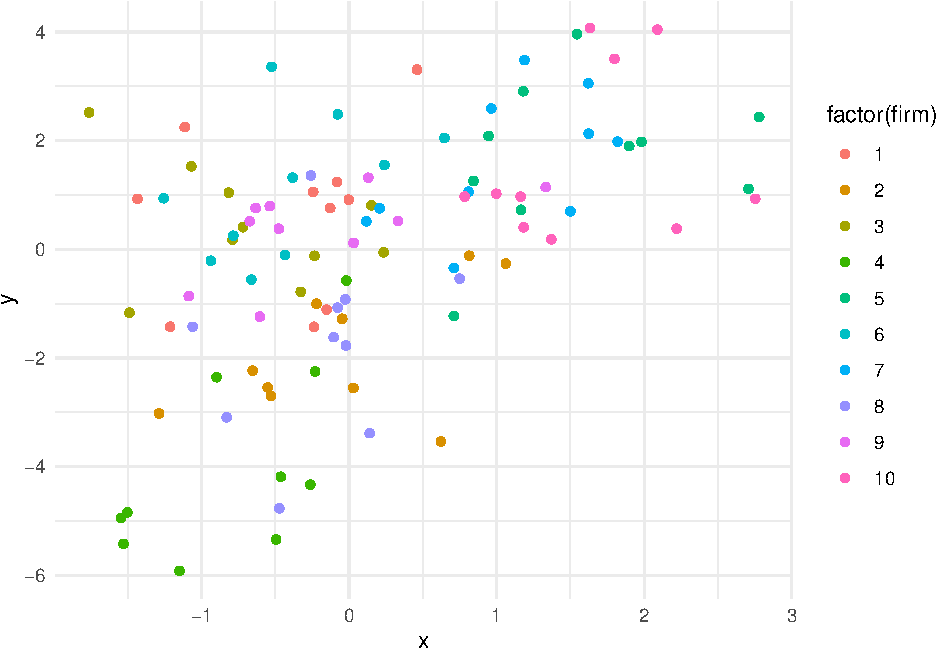
\includegraphics[keepaspectratio]{241-Live-Session_files/figure-latex/unnamed-chunk-8-1.pdf}}

\begin{Shaded}
\begin{Highlighting}[]
\NormalTok{model\_1 }\OtherTok{\textless{}{-}}\NormalTok{ pcl[ , }\FunctionTok{lm}\NormalTok{(y }\SpecialCharTok{\textasciitilde{}}\NormalTok{ x)]}

\DocumentationTok{\#\# since i have the lmtest loaded; i can call: }
\FunctionTok{coeftest}\NormalTok{(model\_1, }\AttributeTok{vcov =} \FunctionTok{vcovHC}\NormalTok{(model\_1, }\AttributeTok{type =} \StringTok{\textquotesingle{}const\textquotesingle{}}\NormalTok{))}
\end{Highlighting}
\end{Shaded}

\begin{verbatim}
## 
## t test of coefficients:
## 
##             Estimate Std. Error t value Pr(>|t|)    
## (Intercept) 0.029680   0.028359  1.0466   0.2954    
## x           1.034833   0.028583 36.2041   <2e-16 ***
## ---
## Signif. codes:  0 '***' 0.001 '**' 0.01 '*' 0.05 '.' 0.1 ' ' 1
\end{verbatim}

\begin{Shaded}
\begin{Highlighting}[]
\DocumentationTok{\#\# to estimate a robust se is a one line solution }
\FunctionTok{coeftest}\NormalTok{(model\_1, }\AttributeTok{vcov =} \FunctionTok{vcovHC}\NormalTok{(model\_1, }\AttributeTok{type =} \StringTok{\textquotesingle{}HC3\textquotesingle{}}\NormalTok{))}
\end{Highlighting}
\end{Shaded}

\begin{verbatim}
## 
## t test of coefficients:
## 
##             Estimate Std. Error t value Pr(>|t|)    
## (Intercept) 0.029680   0.028366  1.0463   0.2955    
## x           1.034833   0.028412 36.4223   <2e-16 ***
## ---
## Signif. codes:  0 '***' 0.001 '**' 0.01 '*' 0.05 '.' 0.1 ' ' 1
\end{verbatim}

These two packages are recommended packages and are \textbf{extremely} well used in R. I've been harping on \texttt{data.table} as abig deal, and it is. Lots of people use the frameowrk and it is great. But these two packages -- \texttt{sandwich} and \texttt{lmtest}, are \textbf{core}. There is no disputing that.

There is a specific relationship between the variance-covariance matrix and the standard error. in fact, it is very much like the relationship between the variance and standard error in any other application we've examined so far.

This relationship is the following:

\[
  SE(\hat{\beta}) = \sqrt{diag(vcov)}
\]

So, all we're really doing is making a post-estimation correction to the variance covariance matrix, and then dividing by this new standard error. Quite straightforward. Why would you want to know this little bit? If you're going to run the test yourself, you will want to be able to pull off the SEs from the \texttt{vcovHC} object.

\begin{Shaded}
\begin{Highlighting}[]
\NormalTok{t.numerator   }\OtherTok{\textless{}{-}} \FunctionTok{coef}\NormalTok{(m2)}
\NormalTok{t.denominator }\OtherTok{\textless{}{-}} \FunctionTok{sqrt}\NormalTok{(}\FunctionTok{diag}\NormalTok{(}\FunctionTok{vcov}\NormalTok{(m2)))}
\NormalTok{t.denominator.robust }\OtherTok{\textless{}{-}} \FunctionTok{sqrt}\NormalTok{(}\FunctionTok{diag}\NormalTok{(}\FunctionTok{vcovHC}\NormalTok{(m2, }\AttributeTok{type =} \StringTok{"HC1"}\NormalTok{)))}

\CommentTok{\# t.ratios: }
\CommentTok{\# not robust: }
\NormalTok{t.numerator }\SpecialCharTok{/}\NormalTok{ t.denominator}
\CommentTok{\# robust }
\NormalTok{t.numerator }\SpecialCharTok{/}\NormalTok{ t.denominator.robust}
\end{Highlighting}
\end{Shaded}

But, like as I showed earlier, we can wrap all this up with the \texttt{lmtest} package's call \texttt{coeftest}.

\begin{Shaded}
\begin{Highlighting}[]
\CommentTok{\# coeftest(m2, vcov(m2))}
\CommentTok{\# coeftest(m2, vcovHC(m2))}
\end{Highlighting}
\end{Shaded}

What if we wanted to pretty-print ourselves a table? If we are using stargazer, or other packages, we will need the SEs off that model.

\begin{Shaded}
\begin{Highlighting}[]
\CommentTok{\# m2.se  \textless{}{-} sqrt(diag(vcov(m2)))}
\CommentTok{\# m2.rse \textless{}{-} sqrt(diag(vcovHC(m2, type = "HC1")))}
\CommentTok{\# }
\CommentTok{\# stargazer(m2, m2, se = list(m2.se, m2.rse), }
\CommentTok{\#           type = "latex", header = FALSE)}
\end{Highlighting}
\end{Shaded}

\subsection{What about clustered standard errors?}\label{what-about-clustered-standard-errors}

Ok, now we're a little deeper down the rabbit hole.

As we've talked about, clustered standard errors acknowledge that you've got treatment assigned at the cluster level, and that there may be significant covariance in potential outcomes at that cluster level. If this is the case, then we have functionally fewer observations than we have nominally, and we also have less power to detect an effect.

To estimate clustered standard errors, we use \texttt{sandwich::vcovCL}.

\begin{Shaded}
\begin{Highlighting}[]
\NormalTok{model\_1 }\OtherTok{\textless{}{-}} \FunctionTok{lm}\NormalTok{(y }\SpecialCharTok{\textasciitilde{}}\NormalTok{ x, }\AttributeTok{data =}\NormalTok{ pcl)}

\DocumentationTok{\#\# without clustering }
\FunctionTok{coeftest}\NormalTok{(model\_1, }\FunctionTok{vcovHC}\NormalTok{(model\_1, }\AttributeTok{type =} \StringTok{\textquotesingle{}const\textquotesingle{}}\NormalTok{))}
\end{Highlighting}
\end{Shaded}

\begin{verbatim}
## 
## t test of coefficients:
## 
##             Estimate Std. Error t value Pr(>|t|)    
## (Intercept) 0.029680   0.028359  1.0466   0.2954    
## x           1.034833   0.028583 36.2041   <2e-16 ***
## ---
## Signif. codes:  0 '***' 0.001 '**' 0.01 '*' 0.05 '.' 0.1 ' ' 1
\end{verbatim}

\begin{Shaded}
\begin{Highlighting}[]
\DocumentationTok{\#\# when we cluster}
\FunctionTok{coeftest}\NormalTok{(model\_1, }\FunctionTok{vcovCL}\NormalTok{(model\_1, }\SpecialCharTok{\textasciitilde{}}\NormalTok{ firm, }\AttributeTok{type =} \StringTok{\textquotesingle{}HC3\textquotesingle{}}\NormalTok{))}
\end{Highlighting}
\end{Shaded}

\begin{verbatim}
## 
## t test of coefficients:
## 
##             Estimate Std. Error t value Pr(>|t|)    
## (Intercept) 0.029680   0.067143   0.442   0.6585    
## x           1.034833   0.050816  20.364   <2e-16 ***
## ---
## Signif. codes:  0 '***' 0.001 '**' 0.01 '*' 0.05 '.' 0.1 ' ' 1
\end{verbatim}

Pretty print that.

\begin{Shaded}
\begin{Highlighting}[]
\FunctionTok{stargazer}\NormalTok{(m1, m1, m1,}
          \AttributeTok{se =} \FunctionTok{list}\NormalTok{(}\FunctionTok{sqrt}\NormalTok{(}\FunctionTok{diag}\NormalTok{(}\FunctionTok{vcov}\NormalTok{(m1))), }
                    \FunctionTok{sqrt}\NormalTok{(}\FunctionTok{diag}\NormalTok{(}\FunctionTok{vcovCL}\NormalTok{(m1, }\SpecialCharTok{\textasciitilde{}}\NormalTok{ firm))), }
                    \FunctionTok{sqrt}\NormalTok{(}\FunctionTok{diag}\NormalTok{(}\FunctionTok{vcovCL}\NormalTok{(m1, }\SpecialCharTok{\textasciitilde{}}\NormalTok{ firm }\SpecialCharTok{+}\NormalTok{ year)))),}
          \AttributeTok{type =} \StringTok{\textquotesingle{}text\textquotesingle{}}\NormalTok{,}
          \AttributeTok{header =} \ConstantTok{FALSE}\NormalTok{)}
\end{Highlighting}
\end{Shaded}

\subsection{Treatment by Treatment Interaction}\label{treatment-by-treatment-interaction}

Summarized data is\ldots{} a drag.

In the book, we're provided data about responses to questions from purported constituents. These people who are writing letters are either names ``Colin'' or ``José'' and who are either writing with ``good'' or ``bad'' grammar.

But, the book gives us data of the form:

\begin{longtable}[]{@{}lllll@{}}
\toprule\noalign{}
& Colin & Colin & José & José \\
\midrule\noalign{}
\endhead
\bottomrule\noalign{}
\endlastfoot
\% Received Reply & 52 & 29 & 37 & 34 \\
(N) & (100) & (100) & (100) & (100) \\
\end{longtable}

Can you run inference against a table that is structured like that? How would you run a model against that form of ``data''?

\subsubsection{Recreate Data}\label{recreate-data}

In order to get a model running against this data, we're going to make a dataset that has the same information in it, but that we can actually run a model against.

\begin{enumerate}
\def\labelenumi{\arabic{enumi}.}
\tightlist
\item
  To begin with, what are the units of observation?
\item
  What are the features in the dataset?
\item
  What is the outcome in the dataset and how is it coded?
\end{enumerate}

Once we've been able to name these, we're able to make a \texttt{data.table} that matches this format.

\begin{Shaded}
\begin{Highlighting}[]
\NormalTok{dat }\OtherTok{\textless{}{-}} \FunctionTok{data.table}\NormalTok{(}\AttributeTok{y       =} \FunctionTok{rep}\NormalTok{(}\ConstantTok{NA}\NormalTok{, }\DecValTok{400}\NormalTok{),}
                  \AttributeTok{name    =} \FunctionTok{rep}\NormalTok{(}\ConstantTok{NA}\NormalTok{, }\DecValTok{400}\NormalTok{),}
                  \AttributeTok{grammar =} \FunctionTok{rep}\NormalTok{(}\ConstantTok{NA}\NormalTok{, }\DecValTok{400}\NormalTok{) )}

\NormalTok{dat[ , y }\SpecialCharTok{:=} \FunctionTok{c}\NormalTok{(}\FunctionTok{rep}\NormalTok{(}\DecValTok{1}\NormalTok{, }\DecValTok{52}\NormalTok{), }\FunctionTok{rep}\NormalTok{(}\DecValTok{0}\NormalTok{, }\DecValTok{48}\NormalTok{),}
              \FunctionTok{rep}\NormalTok{(}\DecValTok{1}\NormalTok{, }\DecValTok{29}\NormalTok{), }\FunctionTok{rep}\NormalTok{(}\DecValTok{0}\NormalTok{, }\DecValTok{71}\NormalTok{),}
              \FunctionTok{rep}\NormalTok{(}\DecValTok{1}\NormalTok{, }\DecValTok{37}\NormalTok{), }\FunctionTok{rep}\NormalTok{(}\DecValTok{0}\NormalTok{, }\DecValTok{63}\NormalTok{),}
              \FunctionTok{rep}\NormalTok{(}\DecValTok{1}\NormalTok{, }\DecValTok{34}\NormalTok{), }\FunctionTok{rep}\NormalTok{(}\DecValTok{0}\NormalTok{, }\DecValTok{66}\NormalTok{) )]}

\NormalTok{dat[ , name    }\SpecialCharTok{:=} \FunctionTok{as.factor}\NormalTok{(}\FunctionTok{c}\NormalTok{(}\FunctionTok{rep}\NormalTok{(}\StringTok{"C"}\NormalTok{, }\DecValTok{200}\NormalTok{), }\FunctionTok{rep}\NormalTok{(}\StringTok{"J"}\NormalTok{,}\DecValTok{200}\NormalTok{)))]}
\NormalTok{dat[ , grammar }\SpecialCharTok{:=} \FunctionTok{as.factor}\NormalTok{(}\FunctionTok{rep}\NormalTok{(}\FunctionTok{c}\NormalTok{(}\StringTok{"G"}\NormalTok{, }\StringTok{"B"}\NormalTok{, }\StringTok{"G"}\NormalTok{, }\StringTok{"B"}\NormalTok{), }\AttributeTok{each =} \DecValTok{100}\NormalTok{) )]}

\NormalTok{dat[ , }\StringTok{\textquotesingle{}:=\textquotesingle{}}\NormalTok{(}\AttributeTok{cg =} \FunctionTok{I}\NormalTok{(name }\SpecialCharTok{==} \StringTok{"C"}\NormalTok{) }\SpecialCharTok{*} \FunctionTok{I}\NormalTok{(grammar }\SpecialCharTok{==} \StringTok{"G"}\NormalTok{),}
           \AttributeTok{cb =} \FunctionTok{I}\NormalTok{(name }\SpecialCharTok{==} \StringTok{"C"}\NormalTok{) }\SpecialCharTok{*} \FunctionTok{I}\NormalTok{(grammar }\SpecialCharTok{==} \StringTok{"B"}\NormalTok{),}
           \AttributeTok{jg =} \FunctionTok{I}\NormalTok{(name }\SpecialCharTok{==} \StringTok{"J"}\NormalTok{) }\SpecialCharTok{*} \FunctionTok{I}\NormalTok{(grammar }\SpecialCharTok{==} \StringTok{"G"}\NormalTok{),}
           \AttributeTok{jb =} \FunctionTok{I}\NormalTok{(name }\SpecialCharTok{==} \StringTok{"J"}\NormalTok{) }\SpecialCharTok{*} \FunctionTok{I}\NormalTok{(grammar }\SpecialCharTok{==} \StringTok{"B"}\NormalTok{))}
\NormalTok{   ]}

\NormalTok{dat}
\end{Highlighting}
\end{Shaded}

\begin{verbatim}
##          y   name grammar     cg     cb     jg     jb
##      <num> <fctr>  <fctr> <AsIs> <AsIs> <AsIs> <AsIs>
##   1:     1      C       G      1      0      0      0
##   2:     1      C       G      1      0      0      0
##   3:     1      C       G      1      0      0      0
##   4:     1      C       G      1      0      0      0
##   5:     1      C       G      1      0      0      0
##  ---                                                 
## 396:     0      J       B      0      0      0      1
## 397:     0      J       B      0      0      0      1
## 398:     0      J       B      0      0      0      1
## 399:     0      J       B      0      0      0      1
## 400:     0      J       B      0      0      0      1
\end{verbatim}

If we've got a \texttt{data.table} that matches the format, can we then estimate models that correspond to the models that are written in the book?

The first of these models, which the book and async refer to as a ``saturated model'' have the following form:

\[
Y_{i} = b_{1}L_{i}\overset{Non-Hispanic}{Good\ Grammar} + 
  b_{2}L_{i}\overset{Hispanic}{Good\ Grammar} + 
  b_{3}L_{i}\overset{Non-Hispanic}{Bad\ Grammar} + 
  b_{4}L_{i}\overset{Hispanic}{Bad\ Grammar} + 
  u_{i}
\]

How would you write a regression that produces this output?

\subsubsection{A more common estimating strategy}\label{a-more-common-estimating-strategy}

More commonly, but equivalently, we estimate this same form with a treatment-by-treatment interaction model. This has the functional form:

\[
Y_{i} = \beta_{0} + \beta_{1} J_{i} + \beta_{2} G_{i} + \beta_{3} J_{i}\times G_{i} + u_{i}
\]

Where, in this model \(J_{i}\) is an indicator for the sender signing ``José'', and \(G_{i}\) is an indicator for the sender using ``good grammar''. Finally, the \(J_{i}\times G_{i}\) is meant to imply that these two indicator are interacted with on another.

How would you write a regression that matches this form?

The book claims that this facilitates testing of nuanced hypotheses, specifically like, ``Is the effect of being named Colin or José different if there is poor grammar compared to if there is good grammar? How would you test this?

\subsection{Pre-Test, Post-Test}\label{pre-test-post-test}

The Pre-Test, Post-Test model is the \emph{most core} :metal: experiment design that is out there.

\begin{enumerate}
\def\labelenumi{\arabic{enumi}.}
\tightlist
\item
  How would you represent this in the ``Grammar of Experiments'' that we talked about last week?
\item
  What threats to validity are present in this design? To what extent are they present?
\item
  What type of model would you estimate in order to match the efficiency of the \emph{design} with the efficiency of the model?
\end{enumerate}

\subsubsection{The Difference in Differences Model}\label{the-difference-in-differences-model}

The Difference in Differences model, sometimes referred to as the D-in-D model, or the D\&D model, is the regression equivalent of the paired t-test.

\begin{enumerate}
\def\labelenumi{\arabic{enumi}.}
\tightlist
\item
  The D-in-D model is \emph{extensible} meaning that you can include extra information in the model, as ``good controls'' to try to improve the model performance.
\item
  The D-in-D model is \emph{efficient} because it uses all the possible information from the experiment design in the model. You could also, always analyze your experiment with a simple between-subjects comparison, but it will be noisier if there is variability between subjects.
\end{enumerate}

\begin{Shaded}
\begin{Highlighting}[]
\FunctionTok{library}\NormalTok{(data.table)}
\FunctionTok{library}\NormalTok{(ggplot2)}
\FunctionTok{library}\NormalTok{(here)}
\end{Highlighting}
\end{Shaded}

\begin{verbatim}
## here() starts at /Users/dhughes/teaching/241/info-241-live-session
\end{verbatim}

\section{Heterogeneous Treatment Effects}\label{heterogeneous-treatment-effects}

When we consider heterogeneous treatment effects, we acknowledge that it is very unlikely that every single person reacts to treatment in exactly the same way. But, are there certain \emph{types} of people who always react more strongly to treatment? Are there certain \emph{types} of people who always react less strongly?

How should we go about (a) looking for HTEs; (b) testings for HTEs with nominal p-value coverages; and (c) reporting HTEs to individuals in a way that make sense?

\subsection{Learning Objectives}\label{learning-objectives-6}

At the end of this week, students will be able to

\begin{enumerate}
\def\labelenumi{\arabic{enumi}.}
\tightlist
\item
  Understand what an HTE is, and what it is not.
\item
  Conduct, test, and interpret models with interaction terms as specific tests of hypotheses.
\end{enumerate}

\subsection{Reading and Discussion: Goodson}\label{reading-and-discussion-goodson}

\begin{enumerate}
\def\labelenumi{\arabic{enumi}.}
\tightlist
\item
  Why do we call them A/B tests, rather than experiments? Are you uncomfortable with the idea that companies are experimenting on you? Are you uncomfortable experimenting in your subjects? If there is a gap between your feeling about being experimented \textbf{on} compared to how you feel when you are \textbf{doing} the experimenting, why does this gap exist?
\item
  What is an A/B test in Goodson's estimation?
\item
  How should we know when a test should be determined to be complete? How should we determine that one experience is \emph{causing} different behaviors in our reference population than another experience?
\end{enumerate}

\begin{itemize}
\tightlist
\item
  Can we decide this while we are working through the experiment?
\item
  Can we make this choice when we see the outcome that we thought we were going to see?
\item
  Can we be \emph{sure} that we have set the correct stopping rules ahead of time?
\end{itemize}

\begin{enumerate}
\def\labelenumi{\arabic{enumi}.}
\setcounter{enumi}{3}
\tightlist
\item
  What are the consequences of peaking, and then stopping early, once we have seen the results?
\end{enumerate}

\subsection{Coding and Demo: The Californians}\label{coding-and-demo-the-californians}

\begin{Shaded}
\begin{Highlighting}[]
\FunctionTok{library}\NormalTok{(data.table)}
\FunctionTok{library}\NormalTok{(stargazer)}

\NormalTok{make\_data }\OtherTok{\textless{}{-}} \ControlFlowTok{function}\NormalTok{(sim\_size) \{ }
\NormalTok{    d }\OtherTok{\textless{}{-}} \FunctionTok{data.table}\NormalTok{(}
      \AttributeTok{id              =} \DecValTok{1}\SpecialCharTok{:}\NormalTok{sim\_size,}
      \AttributeTok{cal\_stanford    =} \FunctionTok{rep}\NormalTok{(}\FunctionTok{c}\NormalTok{(}\StringTok{\textquotesingle{}cal\textquotesingle{}}\NormalTok{, }\StringTok{\textquotesingle{}stanford\textquotesingle{}}\NormalTok{), }\AttributeTok{each =}\NormalTok{ sim\_size}\SpecialCharTok{/}\DecValTok{2}\NormalTok{),}
      \AttributeTok{affluence       =} \FunctionTok{c}\NormalTok{(}
        \FunctionTok{sample}\NormalTok{(}\DecValTok{1}\SpecialCharTok{:}\DecValTok{7}\NormalTok{, }\AttributeTok{size =}\NormalTok{ sim\_size}\SpecialCharTok{/}\DecValTok{2}\NormalTok{, }\AttributeTok{replace =}\NormalTok{ T, }\AttributeTok{prob =} \FunctionTok{c}\NormalTok{(.}\DecValTok{1}\NormalTok{, .}\DecValTok{2}\NormalTok{, .}\DecValTok{2}\NormalTok{, .}\DecValTok{2}\NormalTok{, .}\DecValTok{2}\NormalTok{, .}\DecValTok{05}\NormalTok{, .}\DecValTok{05}\NormalTok{)),}
        \FunctionTok{sample}\NormalTok{(}\DecValTok{1}\SpecialCharTok{:}\DecValTok{7}\NormalTok{, }\AttributeTok{size =}\NormalTok{ sim\_size}\SpecialCharTok{/}\DecValTok{2}\NormalTok{, }\AttributeTok{replace =}\NormalTok{ T, }\AttributeTok{prob =} \FunctionTok{c}\NormalTok{(.}\DecValTok{05}\NormalTok{, .}\DecValTok{05}\NormalTok{, .}\DecValTok{05}\NormalTok{, .}\DecValTok{15}\NormalTok{, .}\DecValTok{2}\NormalTok{, .}\DecValTok{2}\NormalTok{, .}\DecValTok{3}\NormalTok{))),       }
      \AttributeTok{founder\_motivation =} \FunctionTok{rnorm}\NormalTok{(sim\_size, }\AttributeTok{mean =} \DecValTok{100}\NormalTok{, }\AttributeTok{sd =} \DecValTok{7}\NormalTok{), }
      \AttributeTok{treatment\_group =} \FunctionTok{sample}\NormalTok{(}\FunctionTok{c}\NormalTok{(}\DecValTok{0}\NormalTok{,}\DecValTok{1}\NormalTok{), sim\_size, }\AttributeTok{replace =} \ConstantTok{TRUE}\NormalTok{)}
\NormalTok{      )}

\NormalTok{    d[ , capital\_access }\SpecialCharTok{:=} \FunctionTok{rnorm}\NormalTok{(sim\_size, }\AttributeTok{mean =}\NormalTok{ d}\SpecialCharTok{$}\NormalTok{affluence, }\AttributeTok{sd =} \DecValTok{2}\NormalTok{)]}
\NormalTok{    d[ , tau            }\SpecialCharTok{:=} \FunctionTok{rnorm}\NormalTok{(sim\_size, }\AttributeTok{mean =} \DecValTok{5} \SpecialCharTok{+} \DecValTok{5}\SpecialCharTok{*}\FunctionTok{I}\NormalTok{(cal\_stanford }\SpecialCharTok{==} \StringTok{\textquotesingle{}cal\textquotesingle{}}\NormalTok{) }\SpecialCharTok{+}\NormalTok{ affluence)]}
\NormalTok{    d[ , founding\_prob  }\SpecialCharTok{:=}\NormalTok{  founder\_motivation }\SpecialCharTok{+}\NormalTok{ tau}\SpecialCharTok{*}\NormalTok{treatment\_group]}
    
    \FunctionTok{return}\NormalTok{(d)}
\NormalTok{\}}
\end{Highlighting}
\end{Shaded}

\begin{Shaded}
\begin{Highlighting}[]
\NormalTok{d }\OtherTok{\textless{}{-}} \FunctionTok{make\_data}\NormalTok{(}\AttributeTok{sim\_size =} \DecValTok{1000}\NormalTok{)}
\end{Highlighting}
\end{Shaded}

\subsubsection{Overall Treatment Effect}\label{overall-treatment-effect}

What is the (unobserved) true average treatment effect? Estimate a model that includes only the treatment effect and interpret all the coefficients.

\begin{Shaded}
\begin{Highlighting}[]
\NormalTok{model\_0 }\OtherTok{\textless{}{-}}\NormalTok{ d[ , }\FunctionTok{lm}\NormalTok{(founding\_prob }\SpecialCharTok{\textasciitilde{}}\NormalTok{ treatment\_group)]}
\end{Highlighting}
\end{Shaded}

\subsubsection{Founder Motivation}\label{founder-motivation}

Estimate a model that includes the (nearly impossible to measure) variable about \texttt{motivation}. What happens to your estimates? Why does this happen?

\begin{Shaded}
\begin{Highlighting}[]
\NormalTok{model\_1 }\OtherTok{\textless{}{-}}\NormalTok{ d[ , }\FunctionTok{lm}\NormalTok{(founding\_prob }\SpecialCharTok{\textasciitilde{}}\NormalTok{ treatment\_group }\SpecialCharTok{+}\NormalTok{ founder\_motivation)]}
\end{Highlighting}
\end{Shaded}

Print these two modeles next to one another and describe what is happening and why.

\begin{itemize}
\tightlist
\item
  Are the intercept terms the same? Why or why not?
\item
  Are the standard errors teh same? Why or why not?
\item
  Are the estimate treatment effects the same? Why or why not?
\end{itemize}

\subsubsection{Subset Models}\label{subset-models}

Subset the data into two groups based on \texttt{cal\_stanford} and estimate
a model that only includes the treatment effects.

Print these two models side by side, and tell me what is going
on.

\begin{Shaded}
\begin{Highlighting}[]
\NormalTok{model\_cal      }\OtherTok{\textless{}{-}}\NormalTok{ d[cal\_stanford }\SpecialCharTok{==} \StringTok{\textquotesingle{}cal\textquotesingle{}}\NormalTok{, }\FunctionTok{lm}\NormalTok{(founding\_prob }\SpecialCharTok{\textasciitilde{}}\NormalTok{ treatment\_group)]}
\NormalTok{model\_stanford }\OtherTok{\textless{}{-}}\NormalTok{ d[cal\_stanford }\SpecialCharTok{==} \StringTok{\textquotesingle{}stanford\textquotesingle{}}\NormalTok{, }\FunctionTok{lm}\NormalTok{(founding\_prob }\SpecialCharTok{\textasciitilde{}}\NormalTok{ treatment\_group)]}

\FunctionTok{stargazer}\NormalTok{(}
\NormalTok{  model\_cal, model\_stanford, }
  \AttributeTok{type =} \StringTok{\textquotesingle{}text\textquotesingle{}}
\NormalTok{)}
\end{Highlighting}
\end{Shaded}

\begin{verbatim}
## 
## ===========================================================
##                                    Dependent variable:     
##                                ----------------------------
##                                       founding_prob        
##                                     (1)            (2)     
## -----------------------------------------------------------
## treatment_group                  13.359***      9.839***   
##                                   (0.636)        (0.661)   
##                                                            
## Constant                         99.804***     100.031***  
##                                   (0.438)        (0.466)   
##                                                            
## -----------------------------------------------------------
## Observations                        500            500     
## R2                                 0.470          0.308    
## Adjusted R2                        0.468          0.307    
## Residual Std. Error (df = 498)     7.104          7.386    
## F Statistic (df = 1; 498)        440.848***    221.810***  
## ===========================================================
## Note:                           *p<0.1; **p<0.05; ***p<0.01
\end{verbatim}

Based on this, would you conclude that these are different? Use the \texttt{confint()} function on each of these models to inform this discussion -- this is a total trap, because there is very weak statistical basis for what you're about to say, but do it anyways.

\subsubsection{Interaction Model To Test}\label{interaction-model-to-test}

The models that you estimated above are extremely intuitive to talk about, and are probably the right models to report to collaborators, especially those who aren't read into this class. \textbf{But}, they don't include a formal statisical test.

To conduct this test, we're going to rely on the \textbf{same model form} as we used for treatment-by-treatment investigations -- the difference in differences model.

Estimate a model that interacts the treatment indicator with the \texttt{cal\_stanford} indicator, and report what you see from this model.

\begin{Shaded}
\begin{Highlighting}[]
\NormalTok{model\_interaction }\OtherTok{\textless{}{-}}\NormalTok{ d[ , }\FunctionTok{lm}\NormalTok{(founding\_prob }\SpecialCharTok{\textasciitilde{}}\NormalTok{ treatment\_group }\SpecialCharTok{*}\NormalTok{ cal\_stanford)]}

\FunctionTok{summary}\NormalTok{(model\_interaction)}
\end{Highlighting}
\end{Shaded}

\begin{verbatim}
## 
## Call:
## lm(formula = founding_prob ~ treatment_group * cal_stanford)
## 
## Residuals:
##      Min       1Q   Median       3Q      Max 
## -23.7099  -4.8896  -0.2101   4.9203  24.4802 
## 
## Coefficients:
##                                      Estimate Std. Error t value Pr(>|t|)    
## (Intercept)                           99.8039     0.4468 223.361  < 2e-16 ***
## treatment_group                       13.3588     0.6490  20.583  < 2e-16 ***
## cal_stanfordstanford                   0.2271     0.6394   0.355 0.722564    
## treatment_group:cal_stanfordstanford  -3.5197     0.9172  -3.837 0.000132 ***
## ---
## Signif. codes:  0 '***' 0.001 '**' 0.01 '*' 0.05 '.' 0.1 ' ' 1
## 
## Residual standard error: 7.246 on 996 degrees of freedom
## Multiple R-squared:  0.3989, Adjusted R-squared:  0.3971 
## F-statistic: 220.3 on 3 and 996 DF,  p-value: < 2.2e-16
\end{verbatim}

\subsection{? anova}\label{anova}

\subsection{Finally, use the results from model 5 to tell me what the treatment}\label{finally-use-the-results-from-model-5-to-tell-me-what-the-treatment}

\subsection{effect is for males and for californians.}\label{effect-is-for-males-and-for-californians.}

\subsection{}\label{section}

\subsection{AT HOME:}\label{at-home}

\subsection{Work to examine what including the other affluence and literacy}\label{work-to-examine-what-including-the-other-affluence-and-literacy}

\subsection{triggers does to your estimates.}\label{triggers-does-to-your-estimates.}

\subsection{}\label{section-1}

\subsection{Coding and Discussion: Tips at a Restaurant}\label{coding-and-discussion-tips-at-a-restaurant}

\begin{Shaded}
\begin{Highlighting}[]
\DocumentationTok{\#\# Green and Gerber: Question 9.6}
\DocumentationTok{\#\# a, b, and c. }

\NormalTok{d }\OtherTok{\textless{}{-}} \FunctionTok{fread}\NormalTok{(}\StringTok{\textquotesingle{}http://hdl.handle.net/10079/cd6be01a{-}a827{-}4312{-}a2fa{-}74329ce7f96d\textquotesingle{}}\NormalTok{)}

\DocumentationTok{\#\# a. (Probably skip this one)}
\DocumentationTok{\#\#    Suppose that you ignored the gender of the server and simply analyzed whether}
\DocumentationTok{\#\#    the happyface treatment has and effect (and/or) a heterogeneous effects. Use randomization inference }
\DocumentationTok{\#\#    to test whether the Variance of \textbackslash{}tau = 0 using randomization inference by }
\DocumentationTok{\#\#    comparing the variance of potential outcomes in treatment and control. }

\DocumentationTok{\#\# b. Write down a regression model that depicts the effect of the gender of }
\DocumentationTok{\#\#    the waitstaff, whether they put a happyface on the bill, and the interaction }
\DocumentationTok{\#\#    of these factors. }
\DocumentationTok{\#\# }

\DocumentationTok{\#\# c. Estimate the regression model that you wrote down in (b) and test the }
\DocumentationTok{\#\#    interaction between waitstaff and the happyface treatment. }
\DocumentationTok{\#\#    Is the interaction significant. }

\DocumentationTok{\#\# d. Waiting tables in the time of covid: Suppose that you\textquotesingle{}re on the waitstaff }
\DocumentationTok{\#\#    at this restaurant, and while you\textquotesingle{}re waiting tables you\textquotesingle{}re FULLY garbed }
\DocumentationTok{\#\#    up: facemask, face{-}shield, full operating gown, and so on. }
\DocumentationTok{\#\#    What this means is that you have the choice to reveal a gender identity}
\DocumentationTok{\#\#    that is either "Male" or "Female" to the patrons. }
\DocumentationTok{\#\# }
\DocumentationTok{\#\#    {-} Is there one gender identity that receives higher tips in this restaurant? }
\DocumentationTok{\#\#    {-} Is there a gender that has a higher treatment effect? What is the }
\DocumentationTok{\#\#      test that you would run to assess this? }
\end{Highlighting}
\end{Shaded}

\subsection{Sleeeeeeeeeeeep\ldots{}}\label{sleeeeeeeeeeeep}

Suppose that you've conducted an experiment to evaluate the effectiveness of meditation prior to sleeping. Some people are free to do what they want, while others are assigned to a 10 minute guided mindfulness exercise before they go to bed. Treatment is randomly assigned at the individual-level, and people are placed into their groups (and maintained in those groups) for 10 days; then, after two weeks, the groups are flipped.

\begin{enumerate}
\def\labelenumi{\arabic{enumi}.}
\item
  What does the design of this experiment look like?

  R
  R
\item
  Suppose that you also possess some data about the individuals. Specifically, you collect:
\item
  Their age;
\item
  Their coffee drinking habits;
\item
  Their tea drinking habits;
\item
  The number of people in their bed on a typical weeknight;
\item
  The number of cats they own;
\item
  The number of dogs they own.
\item
  First, is there an effect of treatment? Combine the data that you have on hand to write the first, best model.
\item
  Are there are parts of the population that this is especially effective (or ineffective)? How do you know?
\end{enumerate}

\begin{Shaded}
\begin{Highlighting}[]
\FunctionTok{load}\NormalTok{(}\AttributeTok{file =} \FunctionTok{here}\NormalTok{(}\StringTok{"data"}\NormalTok{, }\StringTok{"sleep\_study.Rdata"}\NormalTok{))}
\end{Highlighting}
\end{Shaded}

\section{Treatment Noncompliance}\label{treatment-noncompliance}

This begins a section of the class where we are going to evaluate what happens when problems creep into the actual experiments that we are conducting. We are first going to look at what happens when we instruct people to take treatment, but they choose not to. Or, when we instruct people to take control, but they choose to take treatment instead.

It might seem, at first, like we should just proceed by analyzing according to the treatment condition that they actually received. However, because we haven't experimentally assigned this condition, this creates an unprincipled estimator.

This doesn't mean that all is lost however. We can redefine the causal quantity that we are estimating, and produce a reliable estimate of this new concept.We're going to present two such concepts this week. The first concept is the idea of the intent to treat effect (the ITT). The second concept is the idea of the treatment effect among compliers, which we will call the CACE.

\subsection{Learning Objectives}\label{learning-objectives-7}

\begin{enumerate}
\def\labelenumi{\arabic{enumi}.}
\tightlist
\item
  \textbf{Recognize} when experimental units have not complied with the treatment assignments they were given, and \textbf{appreciate} that this causes problems for our two-group estimator.
\item
  \textbf{Recover} causal estimators, but for sub-populations of the overall population.
\item
  \textbf{Utilize} a new class of model, the two-stage least squares model, or 2SLS, which is the appropriate model choice when we are dealing with either one- or two-sided non-compliance.
\end{enumerate}

\subsection{Starting conversation}\label{starting-conversation}

Life on campus is exciting! Whether students are involved in affinity groups, advocacy groups, protest groups, or just party groups, student life on campus is exciting. We're not to be left out! We're not to be denied the chance to make our voices heard.

What is there to complain about? How about that ``\emph{god awful}'' sound of the bell-tower ringing every hour on the hour.

Suppose that we are to discuss this \emph{very.} \emph{important.} \emph{issue.} before a panel of the deans and University administration. And, further suppose that in light of global events of the past several years, they're actually amenable to what we're proposing -- cutting off those bells, and providing the Berkeley Carillon player a generous retirement. \href{https://www.youtube.com/watch?v=K_8vta9XDpc}{University Carillonist Video}.

However, there's a catch. They are worried that taking such an action would be detrimental to the student experience on campus, and they would like to measure the causal effect of playing vs.~not playing the Carillon while students are changing classes.

In breakout rooms, please design an experiment that would be able to measure the difference in student experience. You will have to propose a measurement, a timescale for that measurement, and a feasible randomization that \emph{could actually} occur given the real-world constraints that what is at question are loud sounds emanating from a 300 foot tower in the middle of a large, busy campus.

If there are any limitations to what you design, please voice those concerns and talk about why they arise, relative to an \emph{ideal} experiment (that you are probably unable to conduct).

\subsection{Non-compliance Discussion}\label{non-compliance-discussion}

\subsubsection{Setting Terms of Understanding}\label{setting-terms-of-understanding}

\begin{itemize}
\tightlist
\item
  What is does the concept of the \emph{intent to treat} effect mean? When is this ITT measurable? When is the ITT an interesting quantity to estimate? When is it uninteresting?\\
\item
  What is the compliance with treatment assignment? How does someone measure \(ITT_{D}\)? Why do Green and Gerber choose to pick such arcane notation? Why is it necessary to know the compliance rate?\\
\item
  What is the compliers average causal effect (CACE)? Under what conditions is this CACE guaranteed to be \emph{exactly} the same as the ITT? Under what conditions is this CACE larger than the ITT? Under what conditions is it smaller than the ITT?
\item
  Is it possible to estimate the CACE without knowing \emph{specifically} who complied? Is it possible to estimate the CACE without knowing anything about compliance rates?
\end{itemize}

\subsubsection{Where Does Noncompliance Occur}\label{where-does-noncompliance-occur}

Is all of this concern about non-compliance actually a concern? Or, is this just another example of academics getting ahead of themselves and worrying about things that are not actually a concern?

In three distinct breakout groups, please talk about one of the following scenarios.

\begin{enumerate}
\def\labelenumi{\arabic{enumi}.}
\tightlist
\item
  \textbf{You are a MIDS instructor writing online content to cause students to be their best possible data scientist.} In this role, you write curriculum, record lectures and assign readings, and create homework assignments for students to work on. How might compliance issues affect curriculum choices?
\item
  \textbf{You are a non-profit interested in reducing litter at your local surf spot.} In this role, you take steps to raise awareness through signs. How does compliance affect what you are likely to learn in any trial or evaluation of your work? How would you know if someone complies?
\item
  \textbf{You are a publisher seeking to sell more copies of the newest, and best causal estimators textbook.} You propose to use pre-roll advertisements on video streaming services to get the word out about the new book. What are all the ways that you can imagine measuring compliance? Which would you propose to use, and why? How might compliance issues affect what you're able to estimate?
\end{enumerate}

When we come back, each student group will have 5 minutes to talk the other two groups through their scenario, including major risks, opportunities, and learning that they took away from the scenario.

\subsection{Estimating with Non-compliance}\label{estimating-with-non-compliance}

\subsubsection{Estimating with non-compliance}\label{estimating-with-non-compliance-1}

\begin{Shaded}
\begin{Highlighting}[]
\DocumentationTok{\#\# install.packages("AER")      \# this has a nice wrapper for iv regression}
                                \CommentTok{\# but we can do it by hand with VERY little work }

\NormalTok{nrows }\OtherTok{=} \DecValTok{1000}

\NormalTok{d }\OtherTok{\textless{}{-}} \FunctionTok{data.table}\NormalTok{(}
  \AttributeTok{id  =} \DecValTok{1}\SpecialCharTok{:}\NormalTok{nrows, }
  \AttributeTok{y0  =} \FunctionTok{rnorm}\NormalTok{(nrows, }\AttributeTok{mean=}\DecValTok{10}\NormalTok{), }
  \AttributeTok{tau =} \FunctionTok{rnorm}\NormalTok{(nrows, }\AttributeTok{mean=}\DecValTok{5}\NormalTok{)}
\NormalTok{)}

\DocumentationTok{\#\# create a treatment effect}
\NormalTok{d[ , y1 }\SpecialCharTok{:=}\NormalTok{ y0 }\SpecialCharTok{+}\NormalTok{ tau]}

\DocumentationTok{\#\# create an assignment vector and a treatment vector with everybody initially}
\DocumentationTok{\#\# set to be untreated. }
\NormalTok{d[ , assigned }\SpecialCharTok{:=} \FunctionTok{sample}\NormalTok{(}\FunctionTok{rep}\NormalTok{(}\FunctionTok{c}\NormalTok{(}\DecValTok{0}\NormalTok{,}\DecValTok{1}\NormalTok{), }\AttributeTok{each=}\NormalTok{nrows}\SpecialCharTok{/}\DecValTok{2}\NormalTok{))] }\CommentTok{\# z in the book}
\NormalTok{d[ , treated }\SpecialCharTok{:=} \DecValTok{0}\NormalTok{] }

\DocumentationTok{\#\# then, among the people who are assigned to receive treatment, actually }
\DocumentationTok{\#\# treat some of them at random. }
\NormalTok{d[}
\NormalTok{  assigned }\SpecialCharTok{==} \DecValTok{1}\NormalTok{, }
\NormalTok{  treated  }\SpecialCharTok{:=} \FunctionTok{sample}\NormalTok{(}
    \AttributeTok{x=}\DecValTok{1}\SpecialCharTok{:}\DecValTok{0}\NormalTok{, }\AttributeTok{size=}\NormalTok{.N, }\AttributeTok{replace=}\ConstantTok{TRUE}\NormalTok{, }\AttributeTok{prob=}\FunctionTok{c}\NormalTok{(.}\DecValTok{7}\NormalTok{, .}\DecValTok{3}\NormalTok{)}
\NormalTok{    )]}

\DocumentationTok{\#\# finally, observe: }
\DocumentationTok{\#\#   {-} the potential outcomes to treatment for the treatment group; and, }
\DocumentationTok{\#\#   {-} the potential outcomes to control for the control group. }
\NormalTok{d[treated }\SpecialCharTok{==} \DecValTok{1}\NormalTok{, Y }\SpecialCharTok{:=}\NormalTok{ y1]}
\NormalTok{d[treated }\SpecialCharTok{==} \DecValTok{0}\NormalTok{, Y }\SpecialCharTok{:=}\NormalTok{ y0]}
\end{Highlighting}
\end{Shaded}

With this data created, we can confirm that the different between potential outcomes to treatment and control still produces the treatment effect. If it doesn't we've got bigger problems than compliance!

\begin{Shaded}
\begin{Highlighting}[]
\NormalTok{d[ , }\FunctionTok{mean}\NormalTok{(y1 }\SpecialCharTok{{-}}\NormalTok{ y0)]}
\end{Highlighting}
\end{Shaded}

\begin{verbatim}
## [1] 4.990989
\end{verbatim}

But, the data that we have created to this point has all the data in the science table. In real life, we won't get access to all this data; instead, we get access to observing some potential outcomes for one group and some other potential outcomes for another group. Let's create this restricted set of data to ensure that our estimator can recover the population parameter that we're looking for, even though it only has access to a sample of data from that population.

\begin{Shaded}
\begin{Highlighting}[]
\NormalTok{d\_observed }\OtherTok{\textless{}{-}}\NormalTok{ d[ , .(assigned, treated, Y)]}
\end{Highlighting}
\end{Shaded}

Does our estimator for the \(ATE\) produce an unbiased estimator of the population parameter, given this sample of data? We know that the population parameter has a treatment effect of \(5\).

\begin{Shaded}
\begin{Highlighting}[]
\DocumentationTok{\#\# how would you code a simple two{-}group ATE estimator? }
\end{Highlighting}
\end{Shaded}

\subsubsection{Build Estimators}\label{build-estimators}

Suppose that you cannot /actually/ observe whether someone was treated or not. This will require that you suspend reality for a moment, to suppose that we do not have access to the \texttt{treateed} variable.

In this case, what concept \textbf{are} you able to estimate? What concept are you \textbf{not} able to estimate?

\paragraph{Estimate the Intent to Treat Effect}\label{estimate-the-intent-to-treat-effect}

Use a linear model to estimate the intent to treat effect. What variables do you need to produce this estimate, and what subset of the data (up to, and including the full set of data) do you use to produce this estimate?

\begin{itemize}
\tightlist
\item
  What should be the magnitude of your ITT estimator, relative to the actual population average treatment effect that we encoded (i.e.~5)? Why do you anticipate that it will be at this level?
\end{itemize}

\subsubsection{Estimate the Compliance Rate}\label{estimate-the-compliance-rate}

Using the full set of data, estimate the compliance rate in two different ways:

\begin{enumerate}
\def\labelenumi{\arabic{enumi}.}
\tightlist
\item
  Estimate using a \texttt{.N} counter, or \texttt{mean} or some other such simple transformation on the data.table.
\item
  Estimate using a linear model, interpreting the coefficient of that model appropriately.
\end{enumerate}

What are the trade offs to these two different methods?

\subsubsection{Compute the CACE}\label{compute-the-cace}

Because you have the ITT and the compliance rate, estimate the CACE. Once again, compute this compliance rate in several ways.

\begin{enumerate}
\def\labelenumi{\arabic{enumi}.}
\tightlist
\item
  Using a \texttt{.N} counter, or \texttt{mean} or some other such simple transformation on the \textbf{entire} data.table. Once again, you might notice that this does not have a sampling based uncertainty estimate associated with it. You need not code this now, but talk about how you would produce something akin to a standard error for the mean given this data.
\item
  Using a \texttt{.N} counter, or \texttt{mean} or some other such simple transformation on a reasonable \textbf{subset} of the data.table.
\end{enumerate}

\begin{itemize}
\tightlist
\item
  Will the estimate that you produce on this subset of data be larger, smaller, or about the same as the estimate that you produced on the full data?
\item
  Will the estimate of the standard error for the mean be larger, smaller, or about the same as the estimate that you produced on the full data?
\end{itemize}

\begin{enumerate}
\def\labelenumi{\arabic{enumi}.}
\setcounter{enumi}{2}
\tightlist
\item
  Finally, estimate the CACE using two linear models. How, if at all, would you produce an estimate of the sampling based uncertainty of these estimates?
\end{enumerate}

\begin{Shaded}
\begin{Highlighting}[]
\NormalTok{cace\_one   }\OtherTok{\textless{}{-}} \StringTok{\textquotesingle{}fill this in\textquotesingle{}} 
\NormalTok{cace\_two   }\OtherTok{\textless{}{-}} \StringTok{\textquotesingle{}fill this in\textquotesingle{}} 
\NormalTok{cace\_three }\OtherTok{\textless{}{-}} \StringTok{\textquotesingle{}fill this in\textquotesingle{}} 
\end{Highlighting}
\end{Shaded}

How do you feel about the sampling based uncertainty that you can produce with these estimators?

\subsection{Two Stage Least Squares}\label{two-stage-least-squares}

In order to estimate with a reliable standard error, we can turn to two stage least squares.

Two-stage least squares estimators have the benefits of

\begin{enumerate}
\def\labelenumi{\arabic{enumi}.}
\tightlist
\item
  Doing \emph{exactly} the same thing that the \(CACE = ITT / ITT_{d}\); but,
\item
  Doing it in a way that has known standard errors that are quickly and easily computable.
\end{enumerate}

\subsubsection{First Stage}\label{first-stage}

In the first stage we:

\begin{itemize}
\tightlist
\item
  Estimate the proportion of people who are receive treatment as a function of being assigned to treatment.
\item
  In the case of one-sided non compliance this is \emph{exactly} the same thing as estimating the
  ITT\_\{d\}, right?
\end{itemize}

\begin{Shaded}
\begin{Highlighting}[]
\NormalTok{first }\OtherTok{\textless{}{-}} \StringTok{\textquotesingle{}fill this in\textquotesingle{}}
\end{Highlighting}
\end{Shaded}

\begin{Shaded}
\begin{Highlighting}[]
\DocumentationTok{\#\# calculate the fitted values from this regression}
\DocumentationTok{\#\#   {-} that is, just multiply the coefficients that you estimate from the}
\DocumentationTok{\#\#     first stage times the data values. In the event that the exclusion}
\DocumentationTok{\#\#     restriction holds, then these predictions are just orthagonal to every}
\DocumentationTok{\#\#     thing that is not modeled in your data! }
\end{Highlighting}
\end{Shaded}

\subsubsection{Second stage}\label{second-stage}

In the second stage we:

\begin{itemize}
\tightlist
\item
  Estimate the relationship between the predicted values and the outcome.
\item
  This will just tell you how the outcome changes in response to the amount of change that your treatment assignment is able to produce.
\end{itemize}

\begin{Shaded}
\begin{Highlighting}[]
\NormalTok{second }\OtherTok{\textless{}{-}} \StringTok{\textquotesingle{}fill this in\textquotesingle{}}
\CommentTok{\# coeftest(second, vcovHC(second, type = "const")) \#\# these ses might be wrong. }
\end{Highlighting}
\end{Shaded}

\begin{Shaded}
\begin{Highlighting}[]
\DocumentationTok{\#\# I\textquotesingle{}ll note that the standard errors from this "hand{-}rolled" 2SLS will not}
\DocumentationTok{\#\# be correct (due to some accounting issues in the variance between the predictions}
\DocumentationTok{\#\# in the first stage and the second stage.}
\DocumentationTok{\#\#}
\DocumentationTok{\#\# we can fix this by hand {-}{-} though I wouldn\textquotesingle{}t {-}{-} or we can use a library that will}
\DocumentationTok{\#\# do the accounting for us, from the library AER}

\CommentTok{\# library(AER)}
\CommentTok{\# iv.model \textless{}{-} ivreg(Y \textasciitilde{} treated | assigned, data = d2)}
\CommentTok{\# }
\CommentTok{\# coeftest(iv.model, vcov = vcovHC(iv.model, type = "const"))}
\end{Highlighting}
\end{Shaded}

\section{Spillover and Interference}\label{spillover-and-interference}

At the outset of the course, we enumerate three hard-core requirement of an experiment design. In addition to intervening in the world, to produce an unbiased estimator of a treatment effect, we require that an experiment:

\begin{enumerate}
\def\labelenumi{\arabic{enumi}.}
\tightlist
\item
  Assign that intervention to experimental units at random to eliminate the possibility of confounding due to selection bias;
\item
  That one, and only one difference exists between two comparison groups, thereby allowing us to exclude all other possible causes \emph{but for} the feature that we have experimentally assigned; and,
\item
  That the treatment experienced by one experimental unit does not ``interfere'' with the potential outcomes of another unit.
\end{enumerate}

In previous weeks, we've engaged with how to evaluate whether a treatment has been successfully randomized. In this week's materials, we are going to examine what, if anything, we may do in response to interference between units.

There are two possibilities. First, we might design our experiment to minimize the effects of interference between units by re-designing or measuring differently. In doing so, we endeavor to maintain the measurement of an individual-level treatment effect, through a multi-group experiment. Second, we might acknowledge the existence of interference and expand our thinking about what \emph{is} a treatment effect.

\subsection{Learning Objectives}\label{learning-objectives-8}

At the conclusion of this week, student will be able to:

\begin{enumerate}
\def\labelenumi{\arabic{enumi}.}
\tightlist
\item
  \textbf{Articulate} in clear terms what circumstances \emph{are}, and what circumstances \emph{are not} interference events.
\item
  \textbf{Appreciate}, and \textbf{evaluate} the extent that interference between units changes both the concept of a treatment effect, and also how a multi-group measurement's estimates change in response to interference between units.
\item
  \textbf{Identify} common situations where interference is likely to occur, and anticipate some methods of mitigating, ameliorating, or designing in response to this interference.
\end{enumerate}

\subsection{Defining Terms}\label{defining-terms}

\begin{itemize}
\tightlist
\item
  What does it mean for one unit to interfere with another unit?

  \begin{itemize}
  \tightlist
  \item
    If two units communicate with one another, is this interference?
  \item
    If three units are all genetically related to one another, is this interference?
  \item
    If ten units all work in the same building, is this interference?
  \item
    If two partners share a tablet for browsing the internet, is this interference?
  \end{itemize}
\item
  Now, be \emph{very} precise with your language: Using the term ``potential-outcomes'' how do Green and Gerber define interference?
\end{itemize}

\subsection{Defining Notation}\label{defining-notation}

\subsubsection{Identify concepts}\label{identify-concepts}

Until this week, we have used two concepts to describe treatment assignment and application:

\begin{itemize}
\tightlist
\item
  \(Z\) is the assignment to treatment; and,
\item
  \(D\) is the dose received of treatment.
\end{itemize}

What concept is identified in the following notation:

\begin{itemize}
\tightlist
\item
  \(E[Y_{i}(1) | D_{i} = 1]\)? Is this measurable?
\item
  \(E[Y_{i}(1)]\)
\item
  Interpret the expression \(Y_{i}(\mathbf{d}) = Y_{i}(d)\) and explain how it conveys the non-interference assumption.
\end{itemize}

\subsubsection{Classroom Assignments}\label{classroom-assignments}

\textbf{(From Green and Gerber, p.~283)}: Sometimes researcher are reluctant to randomly assign individual students in elementary classrooms because they are concerned that treatments administered to some students are likely to spill over to untreated students in the same classroom.

In an attempt to get around possible violations of the non-interference assumption, they assign classrooms as clusters to treatment and control, and administer the treatment to all students in a classroom.

\begin{enumerate}
\def\labelenumi{\arabic{enumi}.}
\tightlist
\item
  State the interference event that commonly leads researcher to assign an entire classroom to a condition.
\item
  State the interference assumption that is implicitly made when classrooms are cluster random assigned. Where, if anywhere does the researcher assume that spillover exists? Where, if anywhere, does the researcher assume that spillover \textbf{not} exist?
\item
  An \emph{estimand} is the concept that an estimator is attempting to estimate. For example, the ATE estimator produces an unbiased, consistent estimate of the individual-level causal effect. What causal estimand does the clustered design identify? Does this estimand include or exclude spillovers within classrooms? What about spillovers between classrooms? What about spillovers between schools?
\end{enumerate}

\subsubsection{Working with a simple example}\label{working-with-a-simple-example}

Suppose that we are conducting an experiment where we examine the effects of releasing solution sets early to some students in the 241 classroom.

\begin{itemize}
\tightlist
\item
  What form of interference is possible?
\item
  Suppose that \emph{Abby}, \emph{Bobby}, \emph{Cathy} and \emph{David} are all on a project team together. Furthermore, suppose that all members of the team work well together, have an ambitious class project that they are working on, and talk regularly.

  \begin{itemize}
  \tightlist
  \item
    If every one of the students were to be assigned to the control group, name values that are plausible for their completion time on problem set three.
  \item
    Suppose that Abby, Bobby and Cathy are assigned to the control group, but that David is assigned to the treatment group. What do you think will happen in their daily project meeting?

    \begin{itemize}
    \tightlist
    \item
      Suppose that, no matter the empirical reality, you assume that there is no interference within this group. What would you call the value that you observe for Abby, given this assumption? Consistent with what you have said will happen in their daily project meeting, what values are you actually seeing for Abby?
    \item
      What are the consequences for your estimated treatment effect?
    \end{itemize}
  \item
    Suppose that Abby and Bobby are assigned to the control group and that Cathy and David are assigned to the treatment group. What do you think will happen in their daily project meeting?
  \item
    What would you call the value that you observe for Abby, given this assumption? Is it different when both Cathy and David are assigned to treatment compared to when only David is assigned to treatment?
  \end{itemize}
\item
  Given what you have stated about this small world, how many treatment assignment conditions do you have to be aware of?
\end{itemize}

\subsubsection{Working with a more complex example}\label{working-with-a-more-complex-example}

Suppose that we are conducting an experiment where we examine the effects of releasing solution sets early to some students in \textbf{a law school} classroom. Law school is notoriously competitive, and outside one's immediate group of friends, there is little collaboration.

\begin{itemize}
\item
  Suppose that \emph{A}, \emph{B}, \emph{C} and \emph{D} are again friends.
\item
  Suppose that \emph{W}, \emph{X}, \emph{Y} and \emph{Z} are also friends.
\item
  But suppose that the two groups are not friends between groups.
\item
  If \emph{A} receives an exam solution, but \emph{W}, \emph{X}, \emph{Y} and \emph{Z} do not, what would you call the values observed for \emph{W}, \emph{X}, \emph{Y} and \emph{Z}?
\item
  If \emph{A}, \emph{B}, and \emph{C} receive an exam solution, but \emph{D}, \emph{W}, \emph{X}, \emph{Y} and \emph{Z} do not, what would you call the values observed for \emph{D}, \emph{W}, \emph{X}, \emph{Y} and \emph{Z}?
\item
  Given this example, are the potential outcomes for un-curved exam score different for \emph{A} if \emph{W} receives or does not receive a solution?
\item
  Given this example, are the potential outcomes for curved exam score different for \emph{A} if \emph{W} receives or does not receive a solution?
\end{itemize}

\subsection{Within subjects experiments}\label{within-subjects-experiments}

Earlier in the course, we talked about two-group pre-test/post-test experiments. These experiments are exceptionally strong against a large series of threats to identification. And, they form the basis of the expanded topic of a \emph{within-subject} experiment.

\begin{enumerate}
\def\labelenumi{\arabic{enumi}.}
\tightlist
\item
  What \emph{is} a within subject experiment?
\item
  When might you propose that a within subject experiment would be advisable? Why? What is the benefit of a within subject experiment?
\item
  When are within subject experiments difficult to conduct?
\end{enumerate}

Green and Gerber, and the async identify two requirements of within-subjects experiments:

\begin{itemize}
\tightlist
\item
  \textbf{No anticipation}
\item
  \textbf{No persistence}
\end{itemize}

What do these two assumptions mean in terms of what you are measuring at the individual-time level?

\begin{itemize}
\tightlist
\item
  Suppose that you were worried that your experimental units might either anticipate being put into treatment or that the treatment they take might have long-run effects. How might you design a test to see if either of these concerns are present in your design?
\end{itemize}

\subsubsection{Survey Experiments}\label{survey-experiments}

\textbf{(From Green and Gerber, p.285)}: Concerns about interference between units sometimes arise in survey experiments. For example surveys sometimes administer a series of \emph{vignettes} involving people with different attributes. A respondent might be told about a low-income person who is randomly described as white or black; after hearing the description, the respondent is asked to rate whether this person deserves public assistance. The respondent is the presented with a vignette about a second person, again randomly described as white or Black, and asked about whether \emph{this} person deserves public assistance.

This design creates four experiment groups:

\begin{enumerate}
\def\labelenumi{\arabic{enumi}.}
\tightlist
\item
  Two vignettes describing Black beneficiaries;
\item
  Two vignettes describing white beneficiaries;
\item
  A vignette describing a Black beneficiary first, followed by a white beneficiary; and,
\item
  A vignette describing a white beneficiary first, followed by a Black beneficiary.
\end{enumerate}

Suppose that each respondent provides a rating after each vignette.

Questions to answer:

\begin{enumerate}
\def\labelenumi{\arabic{enumi}.}
\tightlist
\item
  Propose a model of potential outcomes that reflects the ways that subjects might respond to the treatment and the sequences in which they are presented. How might you represent this using the \texttt{R\ O\ X\ Y} grammar?
\item
  Using your model of potential outcomes, define all of the ATE or ATEs that a researcher might seek to estimate.
\item
  Suggest an experiment design that could estimate this/these causal estimand(s) using observed data.
\item
  Suppose a researcher analyzing this experiment estimates the average \emph{race effect} by comparing the average evaluation of the white recipient to the average evaluation of the black recipient. Is this a sound approach? Why or why not?
\end{enumerate}

\subsection{Discussing the reading: Blake and Coey (2014)}\label{discussing-the-reading-blake-and-coey-2014}

Here is a link to the \href{https://github.com/UC-Berkeley-I-School/mids-w241/blob/main/readings/Blake.2014.pdf}{reading}.

\begin{itemize}
\item
  What is the treatment, and how does treatment assignment work?
\item
  What is the outcome, and how is it measured?
\item
  How does this experimental setup generate spillovers within an auction?
\item
  What is the naive research strategy that produces a biased estimate in the presence of the spillover?
\item
  Tell a story to explain why the within-auction spillovers might give you upward bias in the measured treatment effect.
\item
  (Optional; harder) How does the experiment generate spillovers between auctions?
\item
  Tell a story to explain why you might get downward bias from between-auction spillovers.
\item
  What is the proposed empirical analysis strategy to reduce the bias?
\item
  What would be a better experimental design to conduct in the first place?
\item
  Do you see an example of a stepped-wedge design in this article? Explain.
\end{itemize}

\subsection{Discussing the reading: Miguel and Kremer (2004)}\label{discussing-the-reading-miguel-and-kremer-2004}

Here is a link to the \href{https://github.com/UC-Berkeley-I-School/mids-w241/blob/main/readings/Miguel.2004.pdf}{reading}.

\begin{itemize}
\tightlist
\item
  What question are Miguel and Kremer trying to answer? Why is this important?\\
\item
  What is the spillover problem in this setting?
\item
  How did doctors get the wrong answer in randomized trials before Miguel and Kremer addressed the spillover problem? (The article refers to this as a double penalty.)
\item
  When not taken into account correctly, did the spillovers to cause underestimation or overestimation of the treatment effect? Explain why.
\item
  Which feature do the authors choose to make their experiment less vulnerable to this spillover problem?
\item
  How do the authors still have a (smaller) spillover problem despite this design decision?
\item
  What was the compliance rate for those whom the researchers intended to treat in 1998?
\item
  Name two kinds of noncompliance described in the article, and say which one was largest.
  Due to noncompliance, we can only measure the CACE rather than the ATE. Why is the CACE just fine for the policy question asked in the article?
\item
  Do you see an example of a stepped-wedge design in this article? Explain.
\end{itemize}

\section{Causality from Observational Data}\label{causality-from-observational-data}

\begin{Shaded}
\begin{Highlighting}[]
\FunctionTok{theme\_set}\NormalTok{(}\FunctionTok{theme\_minimal}\NormalTok{())}
\NormalTok{berkeley\_blue   }\OtherTok{\textless{}{-}} \StringTok{\textquotesingle{}\#003262\textquotesingle{}}
\NormalTok{california\_gold }\OtherTok{\textless{}{-}} \StringTok{\textquotesingle{}\#FDB515\textquotesingle{}}
\end{Highlighting}
\end{Shaded}

\begin{figure}
\centering
\pandocbounded{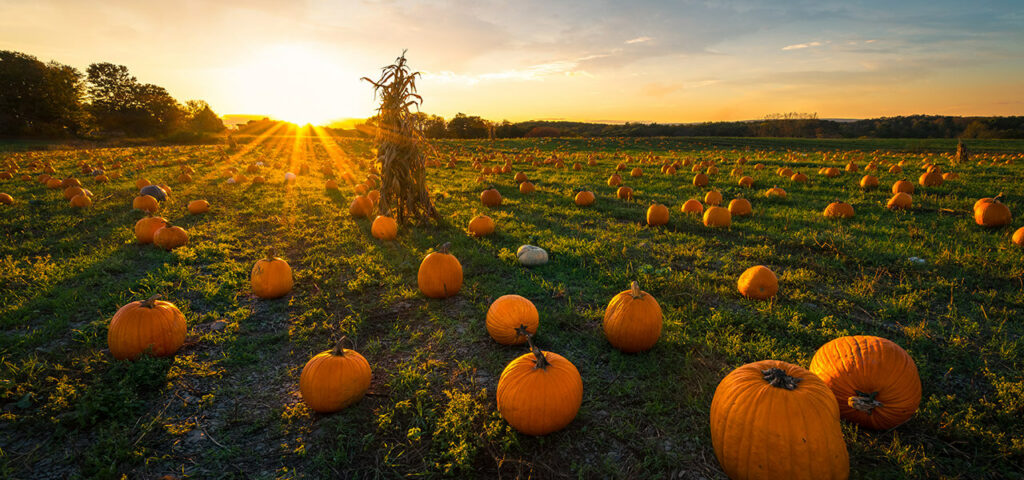
\includegraphics[keepaspectratio]{./images/punkin.jpeg}}
\caption{punkin belly}
\end{figure}

What happens if we cannot run an experiment? Perhaps we don't have the budget or time, perhaps the context is too fraught to conduct an experiment. Should we walk away and learn nothing?

\subsection{Learning Objectives}\label{learning-objectives-9}

At the end of this weeks \emph{extensive} content, students should be able to

\begin{enumerate}
\def\labelenumi{\arabic{enumi}.}
\tightlist
\item
  \textbf{Describe} a series of techniques that have been proposed to estimate causal effects even when a randomized experiment has not been conducted;
\item
  \textbf{Evaluate} whether a particular technique matches with the data generating context;
\item
  \textbf{Analyze} whether an observational data technique is likely to identify a treatment effect; and,
\item
  \textbf{Communicate} the risks and limitations that are brought about when using observational data to make causal claims.
\end{enumerate}

\subsection{The Experimental Ideal}\label{the-experimental-ideal}

If you've been through this once, you've been through it one-hundred times this semester, but it might be worth re-stating what we get out of conducting a randomized experiment.

\begin{quote}
Why do we conduct experiments? What guarantees exist as a result of a well-run experiment?
\end{quote}

\subsection{A Continuum of Plausibility}\label{a-continuum-of-plausibility}

As we are talking today, consider the fully-randomized, full-compliance, full-reporting, high-powered field experiment to be the high-water mark of credibility. Under such a scenario, we can think of any analysis that we undertake as producing a highly-credible, highly-reliable estimate of a treatment effect.

Through our discussion this week, we hope to name where we think other techniques and data generating processes fall relative to this high-water mark. Some, as we will see, might actually produce estimates that are \emph{very nearly} as credible as the experimental ideal. Others are ghastly in their performance.

However, as data scientists who \emph{have to get work done} we need to be able to produce the best possible statement about a treatment effect, and if we have any misgivings about those statements, be able to provide a clear statement about the risk that is attendant to using them.

\subsection{Natural Experiments}\label{natural-experiments}

Natural experiments are experiments that have been conducted by someone \emph{other} than the researcher. If you remember back to Problem Set 1, consider the case of the early childhood education that is provided by the state. When the state \emph{chose} who to provide education to based on need, this was clearly not an experiment because it isn't possible to fully understand the selection criteria used by the state, and so it is not possible to make a strong statement that any estimate produced from a two-group estimator wouldn't be possibly subject to confounding.

But, what about the case where the state \emph{randomly assigned} some kids to get the treatment? Is there any reason that we should discount this simply because it wasn't us to do the assigning? What hubris!

\subsubsection{Questions to consider}\label{questions-to-consider}

\begin{itemize}
\tightlist
\item
  What are the hallmarks of a natural experiment?
\item
  How would you propose to structure your search for natural experiments?
\item
  How will you know when you've actually \emph{found} something that is a natural experiment?
\end{itemize}

\subsubsection{Breakout activity}\label{breakout-activity}

\begin{itemize}
\tightlist
\item
  What are the things in the past year of your lives that have seemed to \emph{arrive at random}? How would you know if they actually \textbf{are} at random?
\item
  After the members of the team have spent a few moments thinking about things that might be random, ask yourselves, ``What might we be able to learn downstream from this experiment?'' What is the most plausible thing that you might learn? What is the longest, most extreme possibility that you might learn?
\end{itemize}

\subsubsection{How does one analyze a natural experiment?}\label{how-does-one-analyze-a-natural-experiment}

If a natural experiment is just a randomization conducted by someone else -- is there anything different that we need to do in order to analyze it? Why or why not?

We talk, with some specificity this week, about estimating using two-stage least squares regression. What is this technique, what does it promise to us, and how does it work?

Consider simulated data that is created in the following way:

\begin{itemize}
\tightlist
\item
  \texttt{ability}, \texttt{family\_income}, and \texttt{lottery} winning to get into a ``magnet'' school are all random
\item
  However, suppose that \texttt{schooling} which is the indicator that someone actually got schooling at a magnet school is correlated with ability, with family income, and with lottery.
\end{itemize}

What would be the consequence of estimating an eventual outcome, using a naive regression?

\begin{Shaded}
\begin{Highlighting}[]
\NormalTok{make\_iv\_data }\OtherTok{\textless{}{-}} \ControlFlowTok{function}\NormalTok{(}\AttributeTok{instrument\_strength=}\FloatTok{1.0}\NormalTok{) \{ }
  \FunctionTok{set.seed}\NormalTok{(}\DecValTok{2}\NormalTok{)}

\NormalTok{  d }\OtherTok{\textless{}{-}} \FunctionTok{data.table}\NormalTok{(}\AttributeTok{id =} \DecValTok{1}\SpecialCharTok{:}\DecValTok{1000}\NormalTok{)}
  
  \DocumentationTok{\#\# These are all independent of one another. }
\NormalTok{  d[ , }\StringTok{\textquotesingle{}:=\textquotesingle{}}\NormalTok{(}
    \AttributeTok{ability       =} \FunctionTok{rnorm}\NormalTok{(.N, }\AttributeTok{mean=}\DecValTok{10}\NormalTok{, }\AttributeTok{sd=}\DecValTok{1}\NormalTok{), }
    \AttributeTok{family\_income =} \FunctionTok{rnorm}\NormalTok{(.N, }\AttributeTok{mean=}\DecValTok{20}\NormalTok{, }\AttributeTok{sd=}\DecValTok{2}\NormalTok{), }
    \AttributeTok{lottery       =} \FunctionTok{rnorm}\NormalTok{(.N, }\AttributeTok{mean=}\DecValTok{10}\NormalTok{, }\AttributeTok{sd=}\DecValTok{1}\NormalTok{) }\SpecialCharTok{\textgreater{}} \DecValTok{10} \DocumentationTok{\#\# Win if larger than 10}
\NormalTok{    )]}
  
  \DocumentationTok{\#\# Create a schooling indicator. This has the following characteristics: }
  \DocumentationTok{\#\#   {-} It is related to winning the lottery (which was random) }
  \DocumentationTok{\#\#   {-} It is related to ability}
  \DocumentationTok{\#\#   {-} It has some "white noise" just so that the model will estimate. }
\NormalTok{  d[ , schooling }\SpecialCharTok{:=}\NormalTok{ instrument\_strength }\SpecialCharTok{*}\NormalTok{ lottery }\SpecialCharTok{+}\NormalTok{ ability }\SpecialCharTok{+} \FunctionTok{rnorm}\NormalTok{(.N, }\AttributeTok{mean=}\DecValTok{0}\NormalTok{, }\AttributeTok{sd=}\DecValTok{1}\NormalTok{)]}
  
  \DocumentationTok{\#\# Create the outcome, which might be earnings. This has the following characteristics: }
  \DocumentationTok{\#\#   {-} It is affected by schooling (Yay!) }
  \DocumentationTok{\#\#   {-} It is affected by ability (Yay!) }
  \DocumentationTok{\#\#   {-} It is affected by family income :| }
  
\NormalTok{  d[ , earnings }\SpecialCharTok{:=} \DecValTok{2} \SpecialCharTok{*}\NormalTok{ schooling }\SpecialCharTok{+}\NormalTok{ ability }\SpecialCharTok{+}\NormalTok{ family\_income }\SpecialCharTok{+}  \FunctionTok{rnorm}\NormalTok{(.N, }\AttributeTok{mean=}\DecValTok{0}\NormalTok{, }\AttributeTok{sd=}\DecValTok{1}\NormalTok{)]}
  \FunctionTok{return}\NormalTok{(d)}
\NormalTok{\}}

\NormalTok{d }\OtherTok{\textless{}{-}} \FunctionTok{make\_iv\_data}\NormalTok{(}\AttributeTok{instrument\_strength =} \FloatTok{1.0}\NormalTok{)}

\NormalTok{model\_wrong }\OtherTok{\textless{}{-}}\NormalTok{ d[ , }\FunctionTok{lm}\NormalTok{(earnings }\SpecialCharTok{\textasciitilde{}}\NormalTok{ schooling)]}
\FunctionTok{coeftest}\NormalTok{(model\_wrong, }\AttributeTok{vcov. =}\NormalTok{ vcovHC)}
\end{Highlighting}
\end{Shaded}

\begin{verbatim}
## 
## t test of coefficients:
## 
##              Estimate Std. Error t value  Pr(>|t|)    
## (Intercept) 24.112215   0.570027  42.300 < 2.2e-16 ***
## schooling    2.566756   0.053039  48.394 < 2.2e-16 ***
## ---
## Signif. codes:  0 '***' 0.001 '**' 0.01 '*' 0.05 '.' 0.1 ' ' 1
\end{verbatim}

\begin{itemize}
\tightlist
\item
  How close, or far from the truth is this estimate? How sure are you that this is different from zero?
\item
  What relationship would you have to change in this data generating process in order to flip the bias of the estimate from estimating a value that is higher than the truth, to estimate a value that is lower than the truth?
\end{itemize}

\subsection{Can we fix this estimate?}\label{can-we-fix-this-estimate}

The promise of two stage-least squares is that it produces unbiased estimates so long as we're able to find something that is random.

\begin{Shaded}
\begin{Highlighting}[]
\NormalTok{first\_stage }\OtherTok{\textless{}{-}}\NormalTok{ d[ , }\FunctionTok{lm}\NormalTok{(schooling }\SpecialCharTok{\textasciitilde{}}\NormalTok{ lottery)] }
\NormalTok{d[ , schooling\_hat}\SpecialCharTok{:=} \FunctionTok{predict}\NormalTok{(first\_stage)] }

\NormalTok{d[ , schooling\_10 }\SpecialCharTok{:=}\NormalTok{ schooling }\SpecialCharTok{\textgreater{}} \DecValTok{10}\NormalTok{]}

\CommentTok{\# d[ , mean(ability), by = .(schooling\_10)]}
\CommentTok{\# d[ , mean(ability), by = .(schooling\_hat)]}
\CommentTok{\# d[ , mean(ability), by = .(lottery)]}

\NormalTok{second\_stage }\OtherTok{\textless{}{-}}\NormalTok{ d[ , }\FunctionTok{lm}\NormalTok{(earnings }\SpecialCharTok{\textasciitilde{}}\NormalTok{ schooling\_hat)]}
\FunctionTok{coeftest}\NormalTok{(second\_stage, }\AttributeTok{vcov. =}\NormalTok{ vcovHC)}
\end{Highlighting}
\end{Shaded}

\begin{verbatim}
## 
## t test of coefficients:
## 
##               Estimate Std. Error t value  Pr(>|t|)    
## (Intercept)   30.46240    2.90018 10.5036 < 2.2e-16 ***
## schooling_hat  1.96857    0.27245  7.2254 9.913e-13 ***
## ---
## Signif. codes:  0 '***' 0.001 '**' 0.01 '*' 0.05 '.' 0.1 ' ' 1
\end{verbatim}

\begin{itemize}
\tightlist
\item
  How or why does this work?
\item
  How does simply making predictions from the first stage regression generate eventual estimates that are unbaised?
\item
  Consider looking at the residuals from the first stage regression
\end{itemize}

\begin{Shaded}
\begin{Highlighting}[]
\NormalTok{d[ , residuals }\SpecialCharTok{:=} \FunctionTok{resid}\NormalTok{(first\_stage)]}

\NormalTok{earnings\_by\_lottery }\OtherTok{\textless{}{-}} 
  \FunctionTok{ggplot}\NormalTok{(d) }\SpecialCharTok{+} 
  \FunctionTok{aes}\NormalTok{(}\AttributeTok{x =}\NormalTok{ earnings, }\AttributeTok{fill =} \FunctionTok{as.factor}\NormalTok{(lottery)) }\SpecialCharTok{+} 
  \FunctionTok{geom\_density}\NormalTok{(}\AttributeTok{alpha =} \FloatTok{0.5}\NormalTok{)}
\NormalTok{earnings\_by\_ability }\OtherTok{\textless{}{-}} 
  \FunctionTok{ggplot}\NormalTok{(d) }\SpecialCharTok{+} 
  \FunctionTok{aes}\NormalTok{(}\AttributeTok{y =}\NormalTok{ earnings, }\AttributeTok{x =}\NormalTok{ ability, }\AttributeTok{color =} \FunctionTok{as.factor}\NormalTok{(lottery)) }\SpecialCharTok{+} 
  \FunctionTok{geom\_point}\NormalTok{()}
\NormalTok{earnings\_by\_family\_income }\OtherTok{\textless{}{-}} 
  \FunctionTok{ggplot}\NormalTok{(d) }\SpecialCharTok{+} 
  \FunctionTok{aes}\NormalTok{(}\AttributeTok{y =}\NormalTok{ earnings, }\AttributeTok{x =}\NormalTok{ family\_income, }\AttributeTok{color =} \FunctionTok{as.factor}\NormalTok{(lottery)) }\SpecialCharTok{+} 
  \FunctionTok{geom\_point}\NormalTok{()}

\NormalTok{earnings\_by\_lottery }\SpecialCharTok{/}\NormalTok{ earnings\_by\_ability }\SpecialCharTok{/}\NormalTok{ earnings\_by\_family\_income}
\end{Highlighting}
\end{Shaded}

\pandocbounded{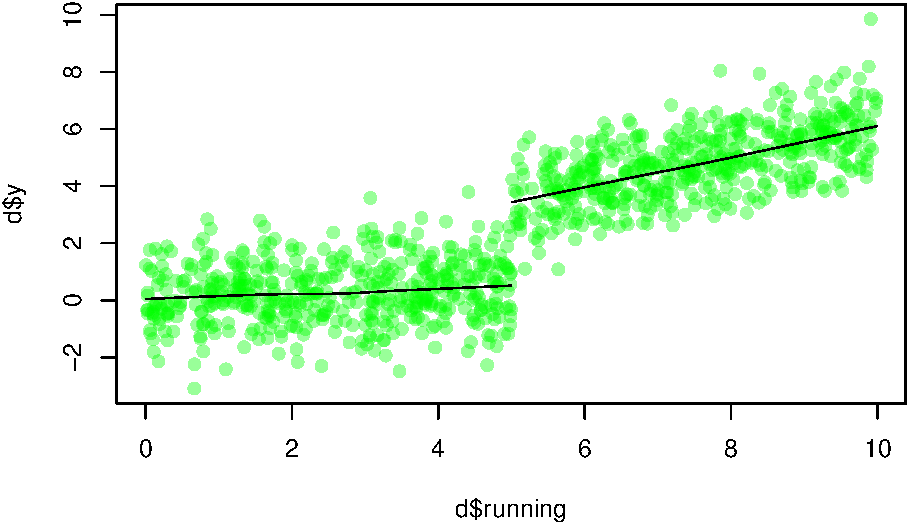
\includegraphics[keepaspectratio]{241-Live-Session_files/figure-latex/unnamed-chunk-23-1.pdf}}

\begin{Shaded}
\begin{Highlighting}[]
\NormalTok{residuals\_lottery }\OtherTok{\textless{}{-}} \FunctionTok{ggplot}\NormalTok{(d) }\SpecialCharTok{+} 
  \FunctionTok{aes}\NormalTok{(}\AttributeTok{x =}\NormalTok{ residuals, }\AttributeTok{fill =} \FunctionTok{as.factor}\NormalTok{(lottery)) }\SpecialCharTok{+} 
  \FunctionTok{geom\_density}\NormalTok{(}\AttributeTok{alpha =} \FloatTok{0.5}\NormalTok{) }\SpecialCharTok{+} 
  \FunctionTok{labs}\NormalTok{(}\AttributeTok{title =} \StringTok{\textquotesingle{}Residuals by lottery\textquotesingle{}}\NormalTok{)}

\NormalTok{residuals\_ability }\OtherTok{\textless{}{-}} \FunctionTok{ggplot}\NormalTok{(d) }\SpecialCharTok{+} 
  \FunctionTok{aes}\NormalTok{(}\AttributeTok{x =}\NormalTok{ residuals, }\AttributeTok{fill =} \FunctionTok{as.factor}\NormalTok{(ability }\SpecialCharTok{\textgreater{}} \DecValTok{10}\NormalTok{)) }\SpecialCharTok{+} 
  \FunctionTok{geom\_density}\NormalTok{(}\AttributeTok{alpha =} \FloatTok{0.5}\NormalTok{) }\SpecialCharTok{+} 
  \FunctionTok{labs}\NormalTok{(}\AttributeTok{title =} \StringTok{\textquotesingle{}Residuals by ability\textquotesingle{}}\NormalTok{)}

\NormalTok{residuals\_lottery }\SpecialCharTok{/}\NormalTok{ residuals\_ability}
\end{Highlighting}
\end{Shaded}

\pandocbounded{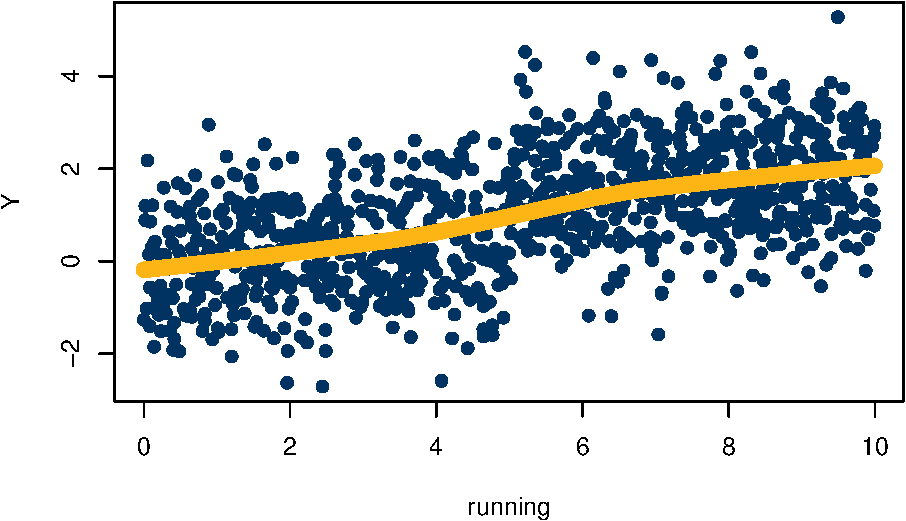
\includegraphics[keepaspectratio]{241-Live-Session_files/figure-latex/unnamed-chunk-24-1.pdf}}

Another way to think about this is in terms of how the predicted values are associated different features. Specifically, consider: Are the predicted values associated with having won the lottery? Are the predicted values associated with ability?

\begin{Shaded}
\begin{Highlighting}[]
\NormalTok{predicted\_lottery }\OtherTok{\textless{}{-}} \FunctionTok{ggplot}\NormalTok{(d) }\SpecialCharTok{+} 
  \FunctionTok{aes}\NormalTok{(}\AttributeTok{x =} \FunctionTok{as.factor}\NormalTok{(lottery), }\AttributeTok{y =}\NormalTok{ schooling\_hat) }\SpecialCharTok{+} 
  \FunctionTok{geom\_jitter}\NormalTok{() }\SpecialCharTok{+} 
  \FunctionTok{labs}\NormalTok{(}\AttributeTok{title =} \StringTok{\textquotesingle{}Predicted Values and Lottery Winning\textquotesingle{}}\NormalTok{) }

\NormalTok{predicted\_ability }\OtherTok{\textless{}{-}} \FunctionTok{ggplot}\NormalTok{(d) }\SpecialCharTok{+} 
  \FunctionTok{aes}\NormalTok{(}\AttributeTok{x =}\NormalTok{ ability, }\AttributeTok{y =}\NormalTok{ schooling\_hat, }\AttributeTok{color =} \FunctionTok{as.factor}\NormalTok{(lottery)) }\SpecialCharTok{+} 
  \FunctionTok{geom\_jitter}\NormalTok{() }\SpecialCharTok{+} 
  \FunctionTok{labs}\NormalTok{(}\AttributeTok{title =} \StringTok{\textquotesingle{}Predicted Values and Ability\textquotesingle{}}\NormalTok{)}

\NormalTok{predicted\_lottery }\SpecialCharTok{/}\NormalTok{ predicted\_ability}
\end{Highlighting}
\end{Shaded}

\pandocbounded{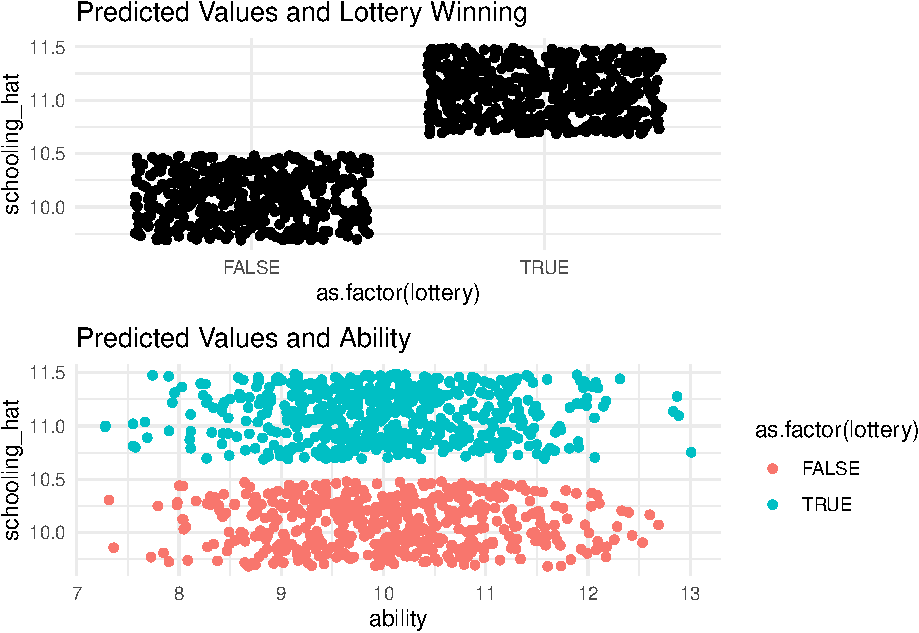
\includegraphics[keepaspectratio]{241-Live-Session_files/figure-latex/unnamed-chunk-25-1.pdf}}

Notice that this entire system works because there is \textbf{some} randomness in the instrument. If there were no randomness in the instrument, or if the instrument had only a small effect on the causal feature that we care about, we will have bias creep back into the estimate.

\begin{quote}
Said another way: This isn't a magic trick that works every time. You \textbf{actually} need randomness, and a strong relationship in order for the the two-stage least squares estimate to work to identify a causal effect.
\end{quote}

\begin{Shaded}
\begin{Highlighting}[]
\NormalTok{d\_weak\_instrument }\OtherTok{\textless{}{-}} \FunctionTok{make\_iv\_data}\NormalTok{(}\AttributeTok{instrument\_strength =}\NormalTok{ .}\DecValTok{1}\NormalTok{)}

\NormalTok{biased\_estimate }\OtherTok{\textless{}{-}}\NormalTok{ d\_weak\_instrument[ , }\FunctionTok{lm}\NormalTok{(earnings }\SpecialCharTok{\textasciitilde{}}\NormalTok{ schooling)]}

\NormalTok{first\_stage }\OtherTok{\textless{}{-}}\NormalTok{ d\_weak\_instrument[ , }\FunctionTok{lm}\NormalTok{(schooling }\SpecialCharTok{\textasciitilde{}}\NormalTok{ lottery)]}
\NormalTok{d\_weak\_instrument[ , schooling\_hat }\SpecialCharTok{:=} \FunctionTok{predict}\NormalTok{(first\_stage)]}

\NormalTok{second\_stage }\OtherTok{\textless{}{-}}\NormalTok{ d\_weak\_instrument[ , }\FunctionTok{lm}\NormalTok{(earnings }\SpecialCharTok{\textasciitilde{}}\NormalTok{ schooling\_hat)]}
\end{Highlighting}
\end{Shaded}

\begin{Shaded}
\begin{Highlighting}[]
\NormalTok{stargazer}\SpecialCharTok{::}\FunctionTok{stargazer}\NormalTok{(}
\NormalTok{  biased\_estimate, second\_stage, }
  \AttributeTok{type =} \StringTok{"text"}
\NormalTok{)}
\end{Highlighting}
\end{Shaded}

\begin{verbatim}
## 
## ===========================================================
##                                    Dependent variable:     
##                                ----------------------------
##                                          earnings          
##                                      (1)            (2)    
## -----------------------------------------------------------
## schooling                          2.645***                
##                                    (0.053)                 
##                                                            
## schooling_hat                                      1.695   
##                                                   (2.635)  
##                                                            
## Constant                          23.587***       33.220   
##                                    (0.543)       (26.712)  
##                                                            
## -----------------------------------------------------------
## Observations                        1,000          1,000   
## R2                                  0.713         0.0004   
## Adjusted R2                         0.713         -0.001   
## Residual Std. Error (df = 998)      2.304          4.302   
## F Statistic (df = 1; 998)        2,483.207***      0.414   
## ===========================================================
## Note:                           *p<0.1; **p<0.05; ***p<0.01
\end{verbatim}

\subsection{Regression Discontinuity}\label{regression-discontinuity}

Regression discontinuity is a \emph{really} clever idea, that when the data presents itself and the analysis is done correctly, provides a \emph{very} compelling argument for having captured a causal effect.

The key insight in the case of regression discontinuity is that we might \emph{not} need something that is actually random in order to produce a credible treatment effect. All we need is treatment assignment mechanism that is not correlated with potential outcomes. And, the argument for regression discontinuity is that if you make a comparison set similar enough along a scoring variable, then it would be very hard for people on one-side or the other-side of an arbitrary point in the scoring variable to be different.

\subsubsection{Why do RDD designs ``work''?}\label{why-do-rdd-designs-work}

\begin{itemize}
\item
  What part of the RDD is producing an unbiased causal estimate?
\item
  Why is this part of he design/data generating process able to produce this unbiased causal estimate?
\item
  What is a ``forcing'' variable?
\item
  How do I identify \emph{where} the cut-point in the forcing variable is located?
\end{itemize}

\subsubsection{Just how common are opportunities for RDD}\label{just-how-common-are-opportunities-for-rdd}

Here's a controversial point of view: Everything that we do as data scientists is to make low-dimensional representations of higher dimensional space. Let's have a jam-session where the class and instructors take turns naming places where a RDD could be run. We'll start with:

\begin{itemize}
\item
  Revolving line of credit -- credit scoring models bring in disparate streams of information, produce a low-dimensional 0-800 (or something like that\ldots) rating and provide revolving lines of credit to different parts of the distribution.
\item
  Now you\ldots{}
\end{itemize}

\subsubsection{Working with Regression Discontinuity Designs}\label{working-with-regression-discontinuity-designs}

Let's look at see what is happening when we're working with RDD designs. To start, let's build some data. Read through each of the lines below, and note what is happening with the data being created. (\emph{Notice that we are chaining together the data.table after we create \texttt{y0} and again after we create \texttt{y1}.})

\begin{Shaded}
\begin{Highlighting}[]
\NormalTok{N }\OtherTok{\textless{}{-}} \DecValTok{1000}

\NormalTok{d }\OtherTok{\textless{}{-}} \FunctionTok{data.table}\NormalTok{(}\AttributeTok{id=}\DecValTok{1}\SpecialCharTok{:}\NormalTok{N)}
\NormalTok{d[ , }\StringTok{\textquotesingle{}:=\textquotesingle{}}\NormalTok{(}
  \AttributeTok{tau     =} \FunctionTok{rnorm}\NormalTok{(.N, }\AttributeTok{mean=}\DecValTok{0}\NormalTok{, }\AttributeTok{sd=}\DecValTok{2}\NormalTok{), }
  \AttributeTok{running =} \FunctionTok{runif}\NormalTok{(.N, }\AttributeTok{min=}\SpecialCharTok{{-}}\DecValTok{2}\NormalTok{, }\AttributeTok{max=}\DecValTok{2}\NormalTok{), }
  \AttributeTok{y0      =} \FunctionTok{runif}\NormalTok{(.N, }\AttributeTok{min=}\SpecialCharTok{{-}}\DecValTok{1}\NormalTok{, }\AttributeTok{max=}\DecValTok{1}\NormalTok{)) ][ , }
\NormalTok{  y1     }\SpecialCharTok{:=}\NormalTok{ y0 }\SpecialCharTok{+}\NormalTok{ tau ][ , }
\NormalTok{  Y      }\SpecialCharTok{:=} \FunctionTok{ifelse}\NormalTok{(running }\SpecialCharTok{\textgreater{}} \DecValTok{0}\NormalTok{, y1, y0)]}
\end{Highlighting}
\end{Shaded}

With the data created, let's quickly look at what we are working with. Does the following plot seem to capture the idea of a treatment effect?

\begin{itemize}
\item
  If so, why?
\item
  If not, why not and how would you propose to change the plot?
\end{itemize}

\begin{Shaded}
\begin{Highlighting}[]
\FunctionTok{ggplot}\NormalTok{(d) }\SpecialCharTok{+} 
  \FunctionTok{aes}\NormalTok{(}\AttributeTok{x=}\NormalTok{running, }\AttributeTok{y=}\NormalTok{Y) }\SpecialCharTok{+} 
  \FunctionTok{geom\_point}\NormalTok{() }\SpecialCharTok{+} 
  \FunctionTok{stat\_smooth}\NormalTok{(}\AttributeTok{method =} \StringTok{\textquotesingle{}lm\textquotesingle{}}\NormalTok{, }\AttributeTok{se=}\ConstantTok{FALSE}\NormalTok{)}
\end{Highlighting}
\end{Shaded}

\begin{verbatim}
## `geom_smooth()` using formula = 'y ~ x'
\end{verbatim}

\pandocbounded{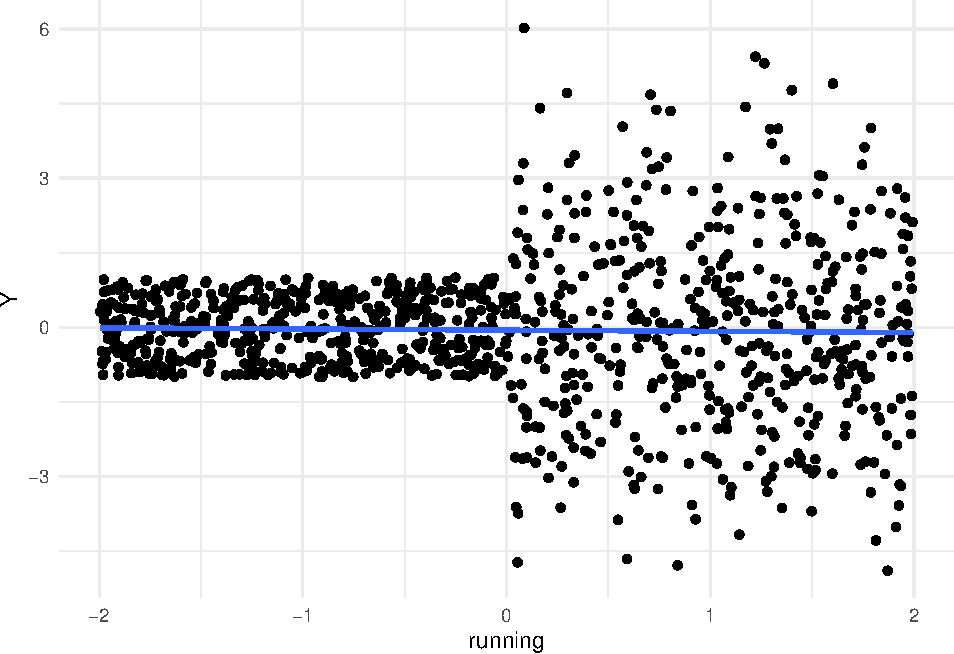
\includegraphics[keepaspectratio]{241-Live-Session_files/figure-latex/first rdd plot-1.pdf}}

We're going to start doing some wacky stuff, subsetting data, and fitting models to subsets of that data. This is behavior that \texttt{ggplot2} takes an opinionated stance against; as such, we're going to work in base plots. Don't worry about the plotting syntax as much as what you're seeing in them.

\begin{Shaded}
\begin{Highlighting}[]
\NormalTok{d[ , }\FunctionTok{plot}\NormalTok{(}\AttributeTok{x=}\NormalTok{running, }\AttributeTok{y=}\NormalTok{Y, }\AttributeTok{pch =} \DecValTok{19}\NormalTok{, }\AttributeTok{col=}\NormalTok{berkeley\_blue)]}
\end{Highlighting}
\end{Shaded}

\begin{verbatim}
## NULL
\end{verbatim}

\begin{Shaded}
\begin{Highlighting}[]
\NormalTok{  d[running }\SpecialCharTok{\textless{}} \DecValTok{0}\NormalTok{, }\FunctionTok{lines}\NormalTok{(}\FunctionTok{lowess}\NormalTok{(running,Y), }\AttributeTok{lwd=}\DecValTok{10}\NormalTok{, }\AttributeTok{col=}\NormalTok{california\_gold)]}
\end{Highlighting}
\end{Shaded}

\begin{verbatim}
## NULL
\end{verbatim}

\begin{Shaded}
\begin{Highlighting}[]
\NormalTok{  d[running }\SpecialCharTok{\textgreater{}} \DecValTok{0}\NormalTok{, }\FunctionTok{lines}\NormalTok{(}\FunctionTok{lowess}\NormalTok{(running,Y), }\AttributeTok{lwd=}\DecValTok{10}\NormalTok{, }\AttributeTok{col=}\NormalTok{california\_gold)]}
\end{Highlighting}
\end{Shaded}

\pandocbounded{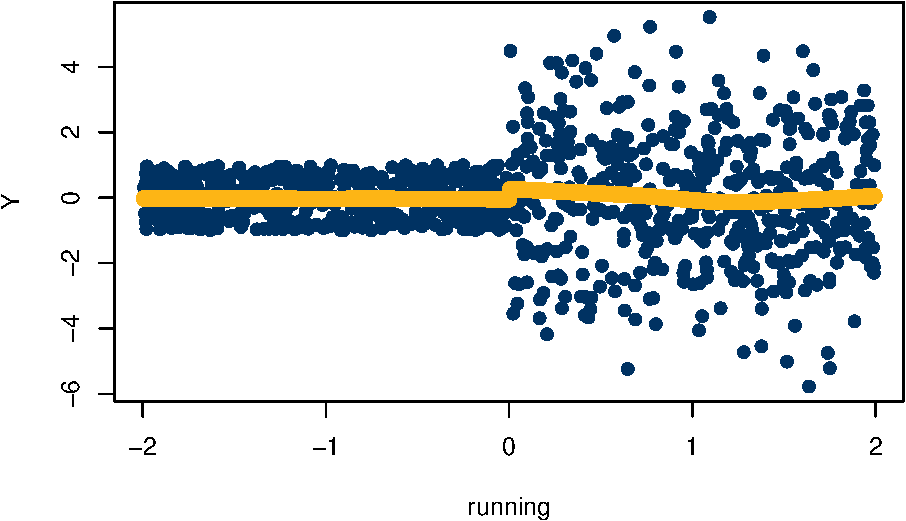
\includegraphics[keepaspectratio]{241-Live-Session_files/figure-latex/second rdd plot-1.pdf}}

\begin{verbatim}
## NULL
\end{verbatim}

This has been \emph{very} fortunate data. There is no trend across the running variable, and things seem mostly linear on both sides. Naturally, the real world is not so tidy.

\subsubsection{More realistic data}\label{more-realistic-data}

\begin{Shaded}
\begin{Highlighting}[]
\NormalTok{d }\OtherTok{\textless{}{-}} \FunctionTok{data.table}\NormalTok{(}\AttributeTok{id=}\DecValTok{1}\SpecialCharTok{:}\NormalTok{N)}

\NormalTok{d[ , }\StringTok{\textquotesingle{}:=\textquotesingle{}}\NormalTok{(}
  \AttributeTok{running =} \FunctionTok{runif}\NormalTok{(}\AttributeTok{n=}\NormalTok{.N, }\AttributeTok{min=}\DecValTok{0}\NormalTok{, }\AttributeTok{max=}\DecValTok{10}\NormalTok{), }
  \AttributeTok{cov1    =} \FunctionTok{rnorm}\NormalTok{(}\AttributeTok{n=}\NormalTok{.N)) ][ ,}
\NormalTok{  Y }\SpecialCharTok{:=}\NormalTok{ running }\SpecialCharTok{*} \FloatTok{0.1} \SpecialCharTok{{-}} \FloatTok{0.2} \SpecialCharTok{*}\NormalTok{ cov1 }\SpecialCharTok{+} \DecValTok{1} \SpecialCharTok{*} \FunctionTok{I}\NormalTok{(running }\SpecialCharTok{\textgreater{}} \DecValTok{5}\NormalTok{) }\SpecialCharTok{+} \FunctionTok{rnorm}\NormalTok{(}\AttributeTok{n=}\NormalTok{.N)]}

\NormalTok{d[ , }\FunctionTok{plot}\NormalTok{(}\AttributeTok{x=}\NormalTok{running, }\AttributeTok{y=}\NormalTok{Y, }\AttributeTok{col=}\NormalTok{berkeley\_blue, }\AttributeTok{pch=}\DecValTok{19}\NormalTok{)]}
\end{Highlighting}
\end{Shaded}

\pandocbounded{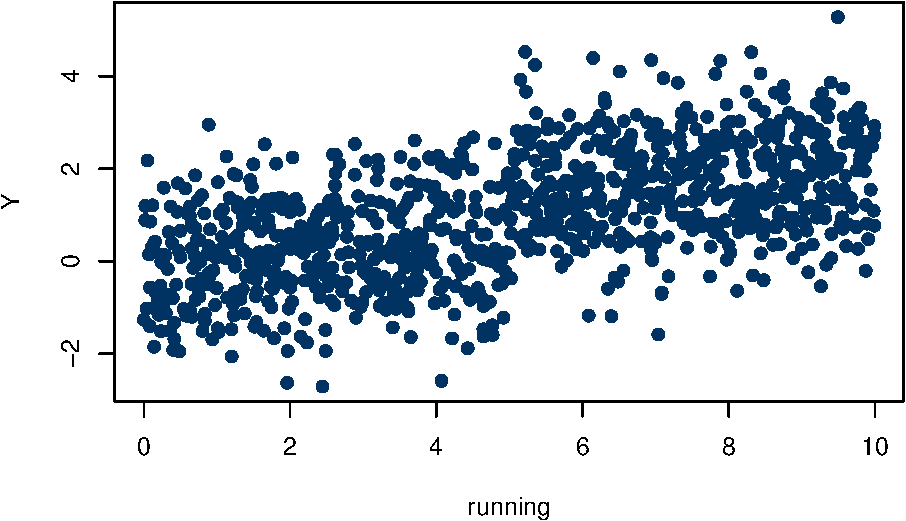
\includegraphics[keepaspectratio]{241-Live-Session_files/figure-latex/slightly more realistic data-1.pdf}}

\begin{verbatim}
## NULL
\end{verbatim}

\begin{itemize}
\item
  Is it clear if there is, or is not an effect in this data simply by looking at it?
\item
  What if you put a smoother through the data?
\end{itemize}

\begin{Shaded}
\begin{Highlighting}[]
\NormalTok{d[ , }\FunctionTok{plot}\NormalTok{(}\AttributeTok{x=}\NormalTok{running, }\AttributeTok{y=}\NormalTok{Y, }\AttributeTok{col=}\NormalTok{berkeley\_blue, }\AttributeTok{pch=}\DecValTok{19}\NormalTok{)]}
\end{Highlighting}
\end{Shaded}

\begin{verbatim}
## NULL
\end{verbatim}

\begin{Shaded}
\begin{Highlighting}[]
\NormalTok{  d[ , }\FunctionTok{lines}\NormalTok{(}\FunctionTok{lowess}\NormalTok{(running, Y), }\AttributeTok{col=}\NormalTok{california\_gold, }\AttributeTok{lwd=}\DecValTok{10}\NormalTok{)]}
\end{Highlighting}
\end{Shaded}

\pandocbounded{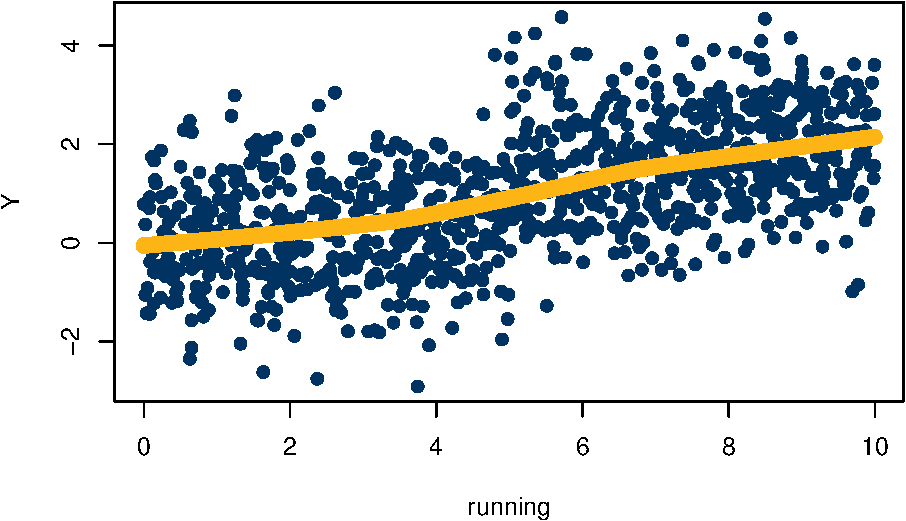
\includegraphics[keepaspectratio]{241-Live-Session_files/figure-latex/unnamed-chunk-28-1.pdf}}

\begin{verbatim}
## NULL
\end{verbatim}

\begin{itemize}
\tightlist
\item
  What if you break that smoother at the policy point?
\end{itemize}

\begin{Shaded}
\begin{Highlighting}[]
\NormalTok{  d[running }\SpecialCharTok{\textless{}} \FloatTok{5.2} \SpecialCharTok{\&}\NormalTok{ running }\SpecialCharTok{\textgreater{}} \FloatTok{4.8}\NormalTok{ , }\FunctionTok{plot}\NormalTok{(}\AttributeTok{x=}\NormalTok{running, }\AttributeTok{y=}\NormalTok{Y, }\AttributeTok{col=}\NormalTok{berkeley\_blue, }\AttributeTok{pch=}\DecValTok{19}\NormalTok{)]}
\end{Highlighting}
\end{Shaded}

\begin{verbatim}
## NULL
\end{verbatim}

\begin{Shaded}
\begin{Highlighting}[]
\NormalTok{    d[running }\SpecialCharTok{\textless{}} \DecValTok{5}\NormalTok{ , }\FunctionTok{lines}\NormalTok{(}\FunctionTok{lowess}\NormalTok{(running, Y), }\AttributeTok{col=}\NormalTok{california\_gold, }\AttributeTok{lwd=}\DecValTok{10}\NormalTok{)]}
\end{Highlighting}
\end{Shaded}

\begin{verbatim}
## NULL
\end{verbatim}

\begin{Shaded}
\begin{Highlighting}[]
\NormalTok{    d[running }\SpecialCharTok{\textgreater{}} \DecValTok{5}\NormalTok{ , }\FunctionTok{lines}\NormalTok{(}\FunctionTok{lowess}\NormalTok{(running, Y), }\AttributeTok{col=}\NormalTok{california\_gold, }\AttributeTok{lwd=}\DecValTok{10}\NormalTok{)]  }
\end{Highlighting}
\end{Shaded}

\pandocbounded{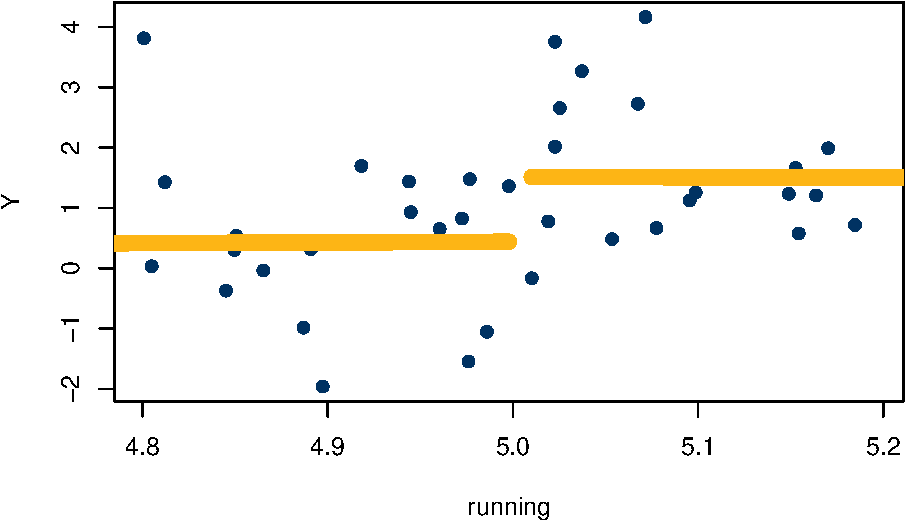
\includegraphics[keepaspectratio]{241-Live-Session_files/figure-latex/unnamed-chunk-29-1.pdf}}

\begin{verbatim}
## NULL
\end{verbatim}

\subsubsection{What about even more challenging data?}\label{what-about-even-more-challenging-data}

\begin{Shaded}
\begin{Highlighting}[]
\NormalTok{d }\OtherTok{\textless{}{-}} \FunctionTok{data.frame}\NormalTok{(}\AttributeTok{running =} \FunctionTok{runif}\NormalTok{(}\DecValTok{1000}\NormalTok{, }\AttributeTok{min =} \DecValTok{0}\NormalTok{, }\AttributeTok{max =} \DecValTok{10}\NormalTok{), }
                \AttributeTok{cov1    =} \FunctionTok{rnorm}\NormalTok{(}\DecValTok{1000}\NormalTok{))}
\NormalTok{d}\SpecialCharTok{$}\NormalTok{y }\OtherTok{\textless{}{-}}\NormalTok{ d}\SpecialCharTok{$}\NormalTok{running }\SpecialCharTok{*} \FloatTok{0.1} \SpecialCharTok{{-}}\NormalTok{ .}\DecValTok{2} \SpecialCharTok{*}\NormalTok{ d}\SpecialCharTok{$}\NormalTok{cov1 }\SpecialCharTok{+} \DecValTok{1} \SpecialCharTok{*} \FunctionTok{I}\NormalTok{(d}\SpecialCharTok{$}\NormalTok{running }\SpecialCharTok{\textgreater{}} \DecValTok{5}\NormalTok{) }\SpecialCharTok{+}
\NormalTok{    .}\DecValTok{4} \SpecialCharTok{*}\NormalTok{ d}\SpecialCharTok{$}\NormalTok{running }\SpecialCharTok{*} \FunctionTok{I}\NormalTok{(d}\SpecialCharTok{$}\NormalTok{running }\SpecialCharTok{\textgreater{}} \DecValTok{5}\NormalTok{) }\SpecialCharTok{+} \FunctionTok{rnorm}\NormalTok{(}\DecValTok{1000}\NormalTok{)}

\FunctionTok{plot}\NormalTok{(}\AttributeTok{x =}\NormalTok{ d}\SpecialCharTok{$}\NormalTok{running, d}\SpecialCharTok{$}\NormalTok{y, }\AttributeTok{pch =} \DecValTok{19}\NormalTok{, }\AttributeTok{col =} \FunctionTok{rgb}\NormalTok{(}\DecValTok{0}\NormalTok{,}\DecValTok{1}\NormalTok{,}\DecValTok{0}\NormalTok{, .}\DecValTok{4}\NormalTok{))}
\FunctionTok{lines}\NormalTok{(}\FunctionTok{lowess}\NormalTok{(d}\SpecialCharTok{$}\NormalTok{running[d}\SpecialCharTok{$}\NormalTok{running }\SpecialCharTok{\textless{}} \DecValTok{5}\NormalTok{], d}\SpecialCharTok{$}\NormalTok{y[d}\SpecialCharTok{$}\NormalTok{running }\SpecialCharTok{\textless{}} \DecValTok{5}\NormalTok{]))}
\FunctionTok{lines}\NormalTok{(}\FunctionTok{lowess}\NormalTok{(d}\SpecialCharTok{$}\NormalTok{running[d}\SpecialCharTok{$}\NormalTok{running }\SpecialCharTok{\textgreater{}} \DecValTok{5}\NormalTok{], d}\SpecialCharTok{$}\NormalTok{y[d}\SpecialCharTok{$}\NormalTok{running }\SpecialCharTok{\textgreater{}} \DecValTok{5}\NormalTok{]))}
\end{Highlighting}
\end{Shaded}

\pandocbounded{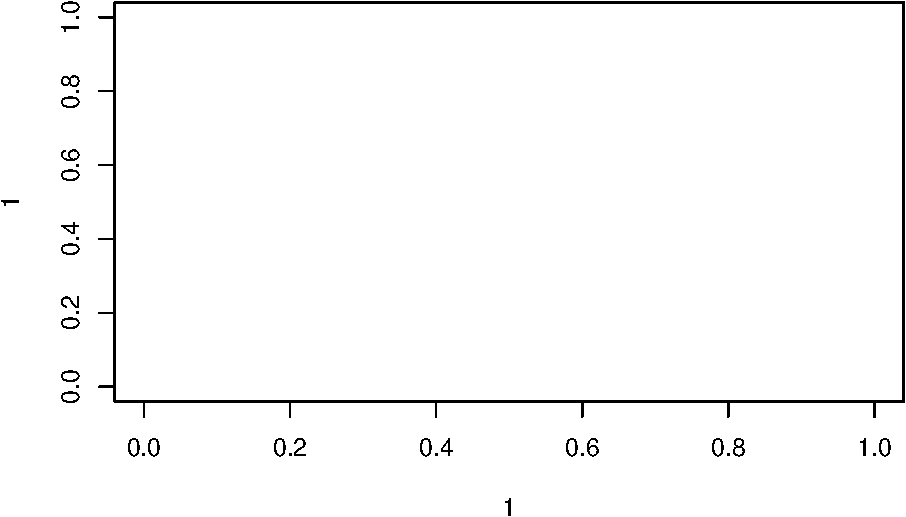
\includegraphics[keepaspectratio]{241-Live-Session_files/figure-latex/unnamed-chunk-30-1.pdf}}

\begin{itemize}
\tightlist
\item
  What model would you fit against this data?
\end{itemize}

\section{Problems and Diagnostics}\label{problems-and-diagnostics}

\begin{figure}
\centering
\pandocbounded{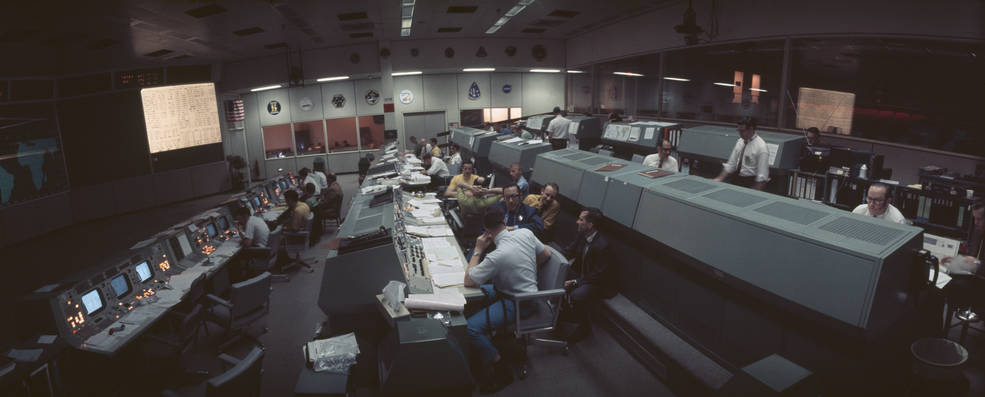
\includegraphics[keepaspectratio]{./images/apollo_13.jpeg}}
\caption{houston, we have a problem}
\end{figure}

\subsection{Learning Objectives}\label{learning-objectives-10}

At the conclusion of this week's live session, students will be able to:

\begin{enumerate}
\def\labelenumi{\arabic{enumi}.}
\tightlist
\item
  \textbf{Recall} and enumerate the several types of problems that might arise in the process of conducting a \emph{real-world} experiment.
\item
  \textbf{Identify} and \textbf{diagnose} when these problems are present in \emph{their} experiment.
\item
  \textbf{Analyze} the consequences of these problems, and communicate to an audience how these problems affect the experiment's ability to produce an unbiased causal estimator.
\item
  \textbf{Propose} a way forward -- how to modify the experiment or modify the estimator.
\end{enumerate}

\subsection{Goals of an Expermient}\label{goals-of-an-expermient}

Recall that the goal of any experiment -- same as the goal for \emph{your} experiment -- is to identify a causal effect that we have a \textbf{guarantee} is unbiased. If we cannot accomplish that, why take the time to conduct the experiment?

Conducting these experiments is \textbf{easy}! At least in a perfect world. The reality is that this world that we live in, and that your data generating process functions within, is far from ``perfect''. And so, as a consequence, machines that we tell to record data fail; people that we tell to take treatment don't actually take it; doses that we think will be sufficient are not; and a litany of other small concerns!

This week's task is to acknowledge that nothing will \emph{ever} be perfect, and then to proactively design our data collection system so that we can diagnose problems when they arise.

\subsection{Problems with Randomization}\label{problems-with-randomization}

Suppose that you are going to conduct an experiment that evaluates the effectiveness of encouragements to complete homework and you have designed the operational details in the following way:

\begin{enumerate}
\def\labelenumi{\arabic{enumi}.}
\tightlist
\item
  You have randomized the list of currently enrolled MIDS 241 students into three treatment groups. Group A will receive \textbf{Always Encouragement}, their instructor will Slack them every day and remind them that Problem Set 4 is coming due; Group B will receive \textbf{Baseline Encouragement}, where they will receive the normal communication from the class; Group C will receive \textbf{Conditional Encouragement}, where students will only be contacted if their grades are below the class average.
\item
  Although you've designed the experiment, contact for students will require that the individual classroom instructors take action to send the encouragements.
\end{enumerate}

\begin{enumerate}
\def\labelenumi{\arabic{enumi}.}
\tightlist
\item
  \textbf{How could this randomization break?} In this breakout, list as many specific ways that you think that the list of people who are assigned to Group A, B, and C might not match those who actually are in the groups. How many ways can you imagine?
\item
  \textbf{What are the consequences?} After listing all the ways that the randomization \emph{could} breakdown, what are the three ways that you think would be more damaging to generating an unbiased causal estimate?
\item
  \textbf{How would you detect?} For these three problems that you've identified, how would you know if the randomization has broken down in this particular way?
\end{enumerate}

\subsection{Placebo Test}\label{placebo-test}

Earlier in the semester, we talked about Placebo Designs, where we intentionally randomize a group of participants and give them a treatment that we do not think will affect outcomes. This placebo treatment, which you might think of as a sugar pill, is designed to allow compliers (and non-compliers) to identify themselves to the experimenting team, producing more efficient estimates of the compliers average causal effect when there is a lot of treatment non-compliance.

This week, we introduce the concept of the \emph{Placebo Test} which, importantly, is different than a \emph{Placebo Design}.

What is a placebo test? How is the concept similar to, and how is it different from, a placebo design?

\begin{itemize}
\tightlist
\item
  How do you know if a particular feature is a good candidate for a placebo test?
\item
  How are placebo tests different from covariate balance checks?
\item
  If you fail a placebo test, why is there more uncertainty about how to fix your experiment?
\end{itemize}

\subsection{Manipulation Check}\label{manipulation-check}

What happens if you don't use a \emph{strong enough} treatment?

\begin{example}

Suppose that you're conducting an experiment to learn the market-value effect of holding a MIDS degree from the School of Information. (Gosh, I sure hope it is positive!) You decide that your experiment is going to send two versions of a resume.

\begin{enumerate}
\def\labelenumi{\arabic{enumi}.}
\tightlist
\item
  \textbf{Version 1 (Control)}: The resume contains the candidate's name, work experience, skills, and a nice statement of their purpose searching for a job. But, the resume does not contain any information about a job candidates master's degree.
\item
  \textbf{Version 2 (Treatment)}: The resume contains the candidate's name, work experience, skills, and a nice statement of their purpose searching for a job. Then, \textbf{after the other materials} the resume lists education at the top of the second page.
\end{enumerate}

\end{example}

\begin{itemize}
\tightlist
\item
  What concerns do you have about the strength of this manipulation? How would you address these concerns?
\item
  What is the maximum manipulation that you can imagine using in this experiment? Are you concerned that there might be \emph{too} much manipulation?
\end{itemize}

\subsection{Advocating for Experimentation}\label{advocating-for-experimentation}

Getting experiments done at work is \emph{almost alwasys} an uphill battle! We won't enumerate the reasons (because we will ask you to do so in a moment), but in our experience, there are some serious impediemnts to getting experiments done.

The good news, from the point of view of your company's leadership: \href{https://venturebeat.com/automation/offerfit-gets-25m-to-kill-a-b-testing-for-marketing-with-machine-learning-personalization/}{A/B Testing is Dead}.

Using the tools of this class and the program, in breakout rooms evaluate this claim. All breakout rooms will read and learn about this claim.

One set will argue in support of the claim: Using new techniques like reinforcement learning and machine generated text, it is possible to determine the most effective messaging without needing to conduct randomized experiments.

The other set of breakout rooms will argue against the claim: While these new techniques might afford some benefits, they cannot replace the work that we've been building over the course of the semester.

\subsubsection{Reasons for and against Experiments}\label{reasons-for-and-against-experiments}

Think about getting an experiment conducted either at work or in your lab.

\begin{itemize}
\tightlist
\item
  What are the reasons that you can identify \emph{in support of} conducting an experiment?
\item
  What are the limitations to, or reasons that you might not conduct an experiment?
\end{itemize}

\section{Attrition, Mediation, and Generalizability}\label{attrition-mediation-and-generalizability}

The theme for this week, as we mention in the async, is that these are \textbf{hard} problems -- in fact, each of these problems are so hard that we do not have an ability to place a clear, numerical answer on \emph{any} of them.

\subsection{Learning Objectives}\label{learning-objectives-11}

At the conclusion of this week, students will be able to

\begin{enumerate}
\def\labelenumi{\arabic{enumi}.}
\tightlist
\item
  \textbf{Recognize} attrition, \textbf{distinguish} the differences between attrition and compliance; \textbf{design} an experimental protocol to minimize the amount of attrition that is present in their data; and \textbf{analyze} an experiment that has experienced attrition to provide best-possible, defensible estimates of treatment.
\item
  \textbf{Reason} about \emph{why} one things causes another; \textbf{reason} about how this affects the ways that they design an experiment or treatment; but, also \textbf{communicate} why it is so difficult to produce clear evidence about \emph{why} something has an effect.
\item
\end{enumerate}

\subsection{Why doesn't mediation analysis work?}\label{why-doesnt-mediation-analysis-work}

Here's a classic case, that is actually very recent. Gaesser et al (2020) present subjects with a short text that describes a stranger in need, for example, someone who has fallen off a motorcycle on the freeway.

\begin{itemize}
\tightlist
\item
  \textbf{Treatment Group} members were asked to imagine helping the person who had fallen of the motorcycle.
\item
  \textbf{Control Group} members were asked to critique the the writing style of the text that they read.
\item
  \textbf{Both Groups} were shown the same text.
\end{itemize}

Unsurprisingly, the authors found that the episodic simulation treatment increased individuals williness to help the stranger in need. But why?

The authors suppose that there are three possible reasons why episodic simulation might work differently.

\begin{enumerate}
\def\labelenumi{\arabic{enumi}.}
\tightlist
\item
  It might work differently depending on how well someone can visualize the scene (\emph{scene vividness}) measured by response to the question, ``The imagined scene of helping in your mind was {[}1. not coherent \ldots{} 7. coherent{]}.''
\item
  It might work differently depending on how well someone can visualize the person (\emph{person vividness}) measured by response to the question, ``Did you visualize the person in your mind?'' {[}1. No, not at all \ldots{} 7. vividly, as if currently there{]}.
\item
  It enables empathetic thought (\emph{perspective taking}) measured by response to the question, ``Did you consider the other person's thoughts and feelings?'' {[}1. No, not at all \ldots{} 7. Strongly considered.{]}
\end{enumerate}

Implicit mediation analysis works in the following way:

\[
  \begin{aligned}
    lm(M &\sim \alpha_{1} + aX_{i} + \epsilon_{1}) \\ 
    lm(Y &\sim \alpha_{2} + cX_{i} + \epsilon_{2}) \\ 
    lm(Y &\sim \alpha_{3} + bM_{i} + c'X_{i} + \epsilon_{3})
  \end{aligned}
\]

Where people talk about \(c\) as the ``total effect'' of \(X\) on \(Y\), and the ``direct effect'' of \(X\) on \(Y\) as the estimate that is reported in \(c'\).

Can you draw this system out in the way that we did in 203? Use circles to represent concepts that you're measuring, and directed arrows to represent causal relationships between these concepts.

\begin{Shaded}
\begin{Highlighting}[]
\FunctionTok{plot}\NormalTok{(}\AttributeTok{x=}\DecValTok{1}\NormalTok{,}\AttributeTok{y=}\DecValTok{1}\NormalTok{, }\AttributeTok{xlim =} \FunctionTok{c}\NormalTok{(}\DecValTok{0}\NormalTok{, }\DecValTok{1}\NormalTok{), }\AttributeTok{ylim =} \FunctionTok{c}\NormalTok{(}\DecValTok{0}\NormalTok{,}\DecValTok{1}\NormalTok{), }\AttributeTok{type =} \StringTok{\textquotesingle{}n\textquotesingle{}}\NormalTok{)}
\end{Highlighting}
\end{Shaded}

\pandocbounded{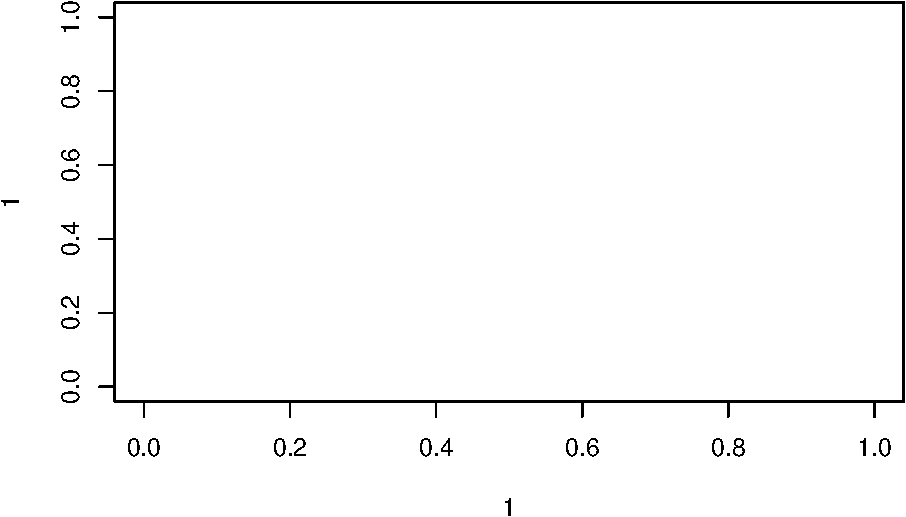
\includegraphics[keepaspectratio]{241-Live-Session_files/figure-latex/unnamed-chunk-33-1.pdf}}

Once you've written out these pathways, what could go wrong in this analysis?

\subsection{Endless Chain of Why?}\label{endless-chain-of-why}

Return back to the example that we talked about at the \emph{very} first week of class, that living in a suburban environment causes a measurable increase in people's BMI. In a five-minute breakout room, produce an enumerated list of theories about \emph{why} living in the suburbs might increase someone's BMI.

\begin{enumerate}
\def\labelenumi{\arabic{enumi}.}
\tightlist
\item
  The team that lists the greatest number possible causes gets a gold star.
\item
  The team that lists the most hilarious possible cause also gets a gold star.
\end{enumerate}

\subsection{Design an experiment to evaluate these possible causes}\label{design-an-experiment-to-evaluate-these-possible-causes}

Now that we've got the list of causes created, and discussed, let's pick a smaller set of the possible causes, and have each group go back into their breakout room for five more minutes to \textbf{specifically} design an experiment that would produce evidence in support of (or in contrast to) their specific theory. Here's the thing: in creating your test, you're trying \textbf{as best as possible} to isolate one, and only one mechanism. So, an experiment that is able to change only a single mechanism is preferred to an experiment that tests who mechanisms at once.

When we come back from this breakout, each team will spend three minutes presenting the design that they produced to test their theory, and the other groups will reason about whether there are other mechanisms that \emph{could} be at play in producing differences in outcomes.

\subsection{Generalizability}\label{generalizability}

Recall the Arizona towel example that we read in \emph{Field Experiments}. It goes something like this, ``There is a door hanger that goes into the bathroom of a Best Western that asks individuals to reuse their towels in an effort to lower environmental impact. There is a large effect in the first period of the study, but there is a smaller, and statistically insignificant effect in the second period of the study.

Bates and Glennerster suggest four misguided approaches that might better be called, ways that other people think about generalizability, but the headings are rather misleading. Recast the headings into four more descriptive sentences instead. I'll do the first for you:

\begin{enumerate}
\def\labelenumi{\arabic{enumi}.}
\tightlist
\item
  An effect learned in a particular context (or location) can never be informative of another location.
\item
\item
\item
\end{enumerate}

Bates and Glenerster suggest a second four-item way to instead reason about generalizability. What are these four steps?

\begin{enumerate}
\def\labelenumi{\arabic{enumi}.}
\tightlist
\item
\item
\item
\item
\end{enumerate}

Describe what each step means?

Now, suppose that you're the decision-maker who has to decide whether to run the experiment signs about towel re-use in Arizona (now for a third trial). How woud you use the four-step framework to evaluate whether to run another experiment?

Throughout the async, David Broockman highlights the extreme difficulty in generating data that tests mechanisms. So, isn't the Bates and Glennerster argument tantamount to saying, ``Just think about this impossible thing that you're never going to be able to measure?'' Or, can you use their framework profitably to generalize to other contexts?

\section{Applications of Experiments}\label{applications-of-experiments}

\subsection{Learning Objectives}\label{learning-objectives-12}

\begin{enumerate}
\def\labelenumi{\arabic{enumi}.}
\tightlist
\item
\item
\item
\end{enumerate}

\section{Review of the Course}\label{review-of-the-course}

\subsection{Learning Objectives}\label{learning-objectives-13}

\begin{enumerate}
\def\labelenumi{\arabic{enumi}.}
\tightlist
\item
\item
\item
\end{enumerate}

\end{document}
